%%%%%%%%%%%%%%%%%%%%%%%%%%%%%%%%%%%%%%%%%
% Masters/Doctoral Thesis 
% LaTeX Template
% Version 2.5 (27/8/17)
%
% This template was downloaded from:
% http://www.LaTeXTemplates.com
%
% Version 2.x major modifications by:
% Vel (vel@latextemplates.com)
%
% This template is based on a template by:
% Steve Gunn (http://users.ecs.soton.ac.uk/srg/softwaretools/document/templates/)
% Sunil Patel (http://www.sunilpatel.co.uk/thesis-template/)
%
% Template license:
% CC BY-NC-SA 3.0 (http://creativecommons.org/licenses/by-nc-sa/3.0/)
%
%%%%%%%%%%%%%%%%%%%%%%%%%%%%%%%%%%%%%%%%%

%----------------------------------------------------------------------------------------
%	PACKAGES AND OTHER DOCUMENT CONFIGURATIONS
%----------------------------------------------------------------------------------------

\documentclass[
11pt, % The default document font size, options: 10pt, 11pt, 12pt
%oneside, % Two side (alternating margins) for binding by default, uncomment to switch to one side
english, % ngerman for German
singlespacing, % Single line spacing, alternatives: onehalfspacing or doublespacing
%draft, % Uncomment to enable draft mode (no pictures, no links, overfull hboxes indicated)
%nolistspacing, % If the document is onehalfspacing or doublespacing, uncomment this to set spacing in lists to single
%liststotoc, % Uncomment to add the list of figures/tables/etc to the table of contents
%toctotoc, % Uncomment to add the main table of contents to the table of contents
%parskip, % Uncomment to add space between paragraphs
%nohyperref, % Uncomment to not load the hyperref package
headsepline, % Uncomment to get a line under the header
%chapterinoneline, % Uncomment to place the chapter title next to the number on one line
%consistentlayout, % Uncomment to change the layout of the declaration, abstract and acknowledgements pages to match the default layout
]{MastersDoctoralThesis} % The class file specifying the document structure

\usepackage[utf8]{inputenc} % Required for inputting international characters
\usepackage[T1]{fontenc} % Output font encoding for international characters

\usepackage{mathpazo} % Use the Palatino font by default

\usepackage[backend=bibtex,style=authoryear,natbib=true]{biblatex} % Use the bibtex backend with the authoryear citation style (which resembles APA)

\addbibresource{bibl.bib} % The filename of the bibliography

\usepackage[autostyle=true]{csquotes} % Required to generate language-dependent quotes in the bibliography


%-------------AXEL PACKAGES----------------------
\usepackage{graphicx}
\usepackage{amsmath}

\usepackage{xcolor}
\usepackage{amssymb}
\usepackage{amsmath}
\usepackage{subcaption}
\usepackage[ruled,vlined]{algorithm2e}
\usepackage{algpseudocode}
\usepackage{hyperref}
\newcolumntype{L}{>{\centering\arraybackslash}m{3.5cm}}
\newcolumntype{M}{>{\centering\arraybackslash}m{2.0cm}}
\usepackage{rotating}
\usepackage{tikz}
\usepackage{multicol}
\graphicspath{{../figs/}}
\newtheorem{proof}{Proof}
\newtheorem{lemma}{Lemma}
\usepackage{comment} 
%----------------------------------------------------------------------------------------
%	MARGIN SETTINGS
%----------------------------------------------------------------------------------------

\geometry{
	paper=a4paper, % Change to letterpaper for US letter
	inner=2.5cm, % Inner margin
	outer=2.5cm, % Outer margin
	bindingoffset=.5cm, % Binding offset
	top=1.5cm, % Top margin
	bottom=1.5cm, % Bottom margin
	%showframe, % Uncomment to show how the type block is set on the page
}

%----------------------------------------------------------------------------------------
%	THESIS INFORMATION
%----------------------------------------------------------------------------------------

\thesistitle{Sequential Cognition Processes: A Framework For Reasoning with Non-Monotonic Logics} % Your thesis title, this is used in the title and abstract, print it elsewhere with \ttitle
\supervisor{Dr. Marco \textsc{Ragni}} % Your supervisor's name, this is used in the title page, print it elsewhere with \supname
\examiner{} % Your examiner's name, this is not currently used anywhere in the template, print it elsewhere with \examname
\degree{Master of Computer Science} % Your degree name, this is used in the title page and abstract, print it elsewhere with \degreename
\author{Axel \textsc{Ind}} % Your name, this is used in the title page and abstract, print it elsewhere with \authorname
\addresses{} % Your address, this is not currently used anywhere in the template, print it elsewhere with \addressname

\subject{Computer Science} % Your subject area, this is not currently used anywhere in the template, print it elsewhere with \subjectname
\keywords{} % Keywords for your thesis, this is not currently used anywhere in the template, print it elsewhere with \keywordnames
\university{\href{https://www.uni-freiburg.de}{Albert-Ludwigs-Universit{\"a}t Freiburg}} % Your university's name and URL, this is used in the title page and abstract, print it elsewhere with \univname
\department{\href{http://www.informatik.uni-freiburg.de}{Department of Computer Science}} % Your department's name and URL, this is used in the title page and abstract, print it elsewhere with \deptname
\group{\href{https://www.cognitive-computation.uni-freiburg.de}{Cognitive Computation}} % Your research group's name and URL, this is used in the title page, print it elsewhere with \groupname
\faculty{\href{http://www.tf.uni-freiburg.de}{Faculty of Engineering}} % Your faculty's name and URL, this is used in the title page and abstract, print it elsewhere with \facname

\AtBeginDocument{
\hypersetup{pdftitle=\ttitle} % Set the PDF's title to your title
\hypersetup{pdfauthor=\authorname} % Set the PDF's author to your name
\hypersetup{pdfkeywords=\keywordnames} % Set the PDF's keywords to your keywords
}

\begin{document}

\frontmatter % Use roman page numbering style (i, ii, iii, iv...) for the pre-content pages

\pagestyle{plain} % Default to the plain heading style until the thesis style is called for the body content

%----------------------------------------------------------------------------------------
%	TITLE PAGE
%----------------------------------------------------------------------------------------

\begin{titlepage}
\begin{center}

\vspace*{.06\textheight}
{\scshape\LARGE \univname\par}\vspace{1.5cm} % University name
\textsc{\Large Master's Thesis}\\[0.5cm] % Thesis type

\HRule \\[0.4cm] % Horizontal line
{\huge \bfseries \ttitle\par}\vspace{0.4cm} % Thesis title
\HRule \\[1.5cm] % Horizontal line
 
\begin{minipage}[t]{0.4\textwidth}
\begin{flushleft} \large
\emph{Author:}\\
\href{http://www.johnsmith.com}{\authorname} % Author name - remove the \href bracket to remove the link
\end{flushleft}
\end{minipage}
\begin{minipage}[t]{0.4\textwidth}
\begin{flushright} \large
\emph{Supervisor:} \\
\href{http://www.jamessmith.com}{\supname} % Supervisor name - remove the \href bracket to remove the link  
\end{flushright}
\end{minipage}\\[3cm]
 
\vfill

\large \textit{A thesis submitted in fulfillment of the requirements\\ for the degree of \degreename}\\[0.3cm] % University requirement text
\textit{in the}\\[0.4cm]
\groupname\\\deptname\\[2cm] % Research group name and department name
 
\vfill

{\large \today}\\[4cm] % Date
%\includegraphics{Logo} % University/department logo - uncomment to place it
 
\vfill
\end{center}
\end{titlepage}

%----------------------------------------------------------------------------------------
%	DECLARATION PAGE
%----------------------------------------------------------------------------------------

\begin{declaration}
\addchaptertocentry{\authorshipname} % Add the declaration to the table of contents
\noindent I, \authorname, declare that this thesis titled, \enquote{\ttitle} and the work presented in it are my own. I confirm that:

\begin{itemize} 
\item This work was done wholly or mainly while in candidature for a research degree at this University.
\item Where any part of this thesis has previously been submitted for a degree or any other qualification at this University or any other institution, this has been clearly stated.
\item Where I have consulted the published work of others, this is always clearly attributed.
\item Where I have quoted from the work of others, the source is always given. With the exception of such quotations, this thesis is entirely my own work.
\item I have acknowledged all main sources of help.
\item Where the thesis is based on work done by myself jointly with others, I have made clear exactly what was done by others and what I have contributed myself.\\
\end{itemize}
 
\noindent Signed:\\
\rule[0.5em]{25em}{0.5pt} % This prints a line for the signature
 
\noindent Date:\\
\rule[0.5em]{25em}{0.5pt} % This prints a line to write the date
\end{declaration}

\cleardoublepage

%----------------------------------------------------------------------------------------
%	QUOTATION PAGE
%----------------------------------------------------------------------------------------

\vspace*{0.2\textheight}

\noindent\enquote{\itshape Everything should be made as simple as possible, but no simpler.}\bigbreak

\hfill Albert Einstein

%----------------------------------------------------------------------------------------
%	ABSTRACT PAGE
%----------------------------------------------------------------------------------------

\begin{abstract}
\addchaptertocentry{\abstractname} % Add the abstract to the table of contents
Approaches to cognitive modelling with non-monotonic logics have thus far been largely \textit{ad hoc} and poorly standardised, making inter-model comparisons difficult. As an attempt to systematically represent non-monotonic logics in a framework that standardises cognitive modelling under these logics without sacrificing their expressiveness, we introduce the Sequential Cognition Process (SCP). Under the assumption that human reasoning can be represented as a sequence of distinct cognitive operations on an initial knowledge base, SCPs provide a consistent framework for generating and evaluating models of human cognition. Using an adapted interpretation of the Weak Completion Semantics (WCS) and Reiter's Default Logic, SCPs are able to accurately model several classical experiments in cognitive modelling. We use the SCP framework to model both general case reasoners -- which arrive at the most frequently observed conclusions -- and poorly-studied individual case reasoners -- which do not. We illustrate the use of the SCP framework through examination of the Wason Selection Task and Suppression Task.
\end{abstract}

%----------------------------------------------------------------------------------------
%	ACKNOWLEDGEMENTS
%----------------------------------------------------------------------------------------

\begin{acknowledgements}
\addchaptertocentry{\acknowledgementname} % Add the  acknowledgements to the table of contents
Special thanks to Dr. Marco Ragni, for his enthusiastic supervision of my ongoing academic studies; Raymond Ind and Julie Ind for their emotional and financial support; and to Anastasia Sushich for her tireless support.
\end{acknowledgements}

%----------------------------------------------------------------------------------------
%	LIST OF CONTENTS/FIGURES/TABLES PAGES
%----------------------------------------------------------------------------------------

\tableofcontents % Prints the main table of contents

\listoffigures % Prints the list of figures

\listoftables % Prints the list of tables

%----------------------------------------------------------------------------------------
%	ABBREVIATIONS
%----------------------------------------------------------------------------------------

\begin{abbreviations}{ll} % Include a list of abbreviations (a table of two columns)

\textbf{SCP} & \textbf{S}equential \textbf{C}ognitive \textbf{P}rocesses\\
\textbf{nSCP} & \textbf{n}on-\textbf{S}equential \textbf{C}ognitive \textbf{P}rocesses\\
\textbf{WCS} & \textbf{W}eak \textbf{C}ompletion \textbf{S}emantics\\
\textbf{WST} & \textbf{W}ason \textbf{S}election \textbf{T}ask \\
\textbf{CTM} & \textbf{C}ognitive \textbf{T}ransition \textbf{M}odel \\
\textbf{pCTM}& \textbf{p}artial \textbf{C}ognitive \textbf{T}ransition \textbf{M}odel
\end{abbreviations}

%----------------------------------------------------------------------------------------
%	THESIS CONTENT - CHAPTERS
%----------------------------------------------------------------------------------------

\mainmatter % Begin numeric (1,2,3...) page numbering

\pagestyle{thesis} % Return the page headers back to the "thesis" style

\chapter{Introduction} \label{chp:intro}
\section{Overview} \label{sec:overview}
% a statement of the problem
The human mind is complex. So complex that thousands of approaches from dozens of fields have failed to capture its complexity. The sheer size of the brain -- containing  over 5000 times as many neurons as the largest practical neural networks \citep{mocanu2018scalable} -- and our limited understanding of the fundamental learning processes it employs mean that researchers can neither completely describe nor predict human actions nor model human thought processes. Instead, much of the current state of the art in cognitive modelling relies on one of two general approaches: creating systems that structurally approximate the human brain, and creating systems which approximate a more abstract intuition of cognition. The first type of system encompasses many algorithms related to machine learning and deep learning; the second type, with which this paper is concerned, has existed in some form for far longer than humans have been thinking creatures \citep{smirnova2015crows}. Every shark stalking its prey, every tiny proto-mammal hiding from a hungry dinosaur, and every man driving to work in the morning, has applied this type of reasoning when trying to make predictions about the actions of other agents in their world. By applying case-specific reasoning to a known world state we are able to make imperfect, but quick, predictions about the mental state of other agents in our world.

Due in part to the difficulty of cloning dinosaurs to hunt participants in cognitive research experiments, and partly due to concerns about the ease with which they could answer questionnaires on the experience later, most cognitive tasks used by researchers tend to be more dull than the examples above.

Non-monotonic logics have proven able to adequately model a large number of standard cognitive reasoning tasks such as The Wason Selection Task\citep{wason1968reasoning} and Suppression Task \citep{byrne1989suppressing}. These approaches, though effective and well-founded in isolation, are often unable to integrate or be compared to data models of other tasks, even when they rely on the same underlying logic. Although the non-monotonic logics themselves are generally carefully described, procedures ranging from best practise in deciding appropriate knowledge bases to the mechanisms by which inferences should be interpreted tend to be re-imagined on a case-by-case basis.

Further, cognitive frameworks using non-monotonic logics are almost always designed to describe the most common (general) conclusion drawn by participants in the experiment. Modelling other individual reasoners or classes of reasoners who differ from the norm is often a non-trivial process. It has been shown that the Weak Completion Semantics \citep{holldobler2015weak} is able model the four most general cases of the Wason Selection Task under the assumption that reasoners who differ from the general case (\textit{deviant reasoners}) follow a sequence of mental processes that is still highly similar to that of the general reasoner \citep{breu2019weak}.

This thesis introduces the Sequential Cognition Process (SCP) which generalises the assumption of sequential cognitive operations, each of which uses a collection of epistemic states as input and produces a collection of epistemic states as output. 


\section{A Review of Terminology} \label{sec:terminology}
% a review of terms
\section{Current State of the Art} \label{sec:soa}
% review of literature
The current state of the art in cognitive modelling using non-monotonic logics has begun to show a shift towards a computational approach to problem solving \citep{dietz2012computational}. \cite{stenning2012human} argued, in a general sense, that modelling human reasoning should be done primarily towards an appropriate representation of the underlying cognitive processes, and secondarily, it should be evaluated empirically with respect to this representation. This philosophy is in stark contrast to that of many other areas of artificial intelligence research, in which the underlying structure of the agent does not need to mimic existing cognitive processes, and instead the primary evaluation criteria is generally the effectiveness of the agent at making predictions on unseen data sets.

This thesis makes extensive reference to the work of \cite{dietz2012computational}, \cite{dietz2014modeling}, \cite{ragni2017wason} and their contributions to the emerging field of cognitive modelling. 

The author of this thesis has previously shown the suitability of the Weak Completion Semantics for modelling individual reasoners in the Wason Selection Task \citep{breu2019weak} and the SCP framework that this thesis introduces is an extension of the intuition of discrete, sequential processes underlying cognition. The question of how to model individual reasoners is a pernicious problem in cognitive modelling and work by \cite{breu2019weak}, as well modelling tools like \texttt{CCOBRA} \citep{ccobra} have been able to use traditional modelling techniques, with minor variations, to replicate more than simply the most common reasoner responses.



\section{Contributions of the SCP Framework} \label{sec:contributions}
Using SCPs and a set of well-founded cognitive operations it is possible to apply traditional search techniques to problems in cognitive modelling with non-monotonic logics that have previously required expert-made models. SCPs introduce a number of desirable properties: they introduce a partially standardised (though extensible) set of allowable cognitive operations, they standardise the structure of what constitutes an epistemic state, they are easily modified to accommodate deviant reasoners when a well-founded general model already exists, and their sequential structure makes them well-suited to scoring algorithms that allow intra- and inter-experimental modelling and comparisons.

Logics which are able to interpret conditionals of the form ``If $\phi$, then $\psi$" are varied in both their implementation and underlying principles. Work by \cite{heit2005defending} has shown evidence that not all information is derived, stored, or retrieved symmetrically and thus, it is unlikely that a single logical system will be able fully model tasks which utilise information whose interpretation is dependant on multiple structurally and interpretationally diverse sources of information. The SCP framework enables researchers to use robust search techniques which make no assumptions about conditional interpretation at formulation time, and rather, branches to incorporate multiple possible epistemic knowledge structures at run-time. This technique, enables multiple non-monotonic logics to be used across a single cognition task.

This thesis also introduces a new method for modelling reasoners in the WST which makes use of the interpretation of a conditional and its contraposition to provide a more intuitive method of applying the WCS to the task. Section~\ref{sec:supSCP} shows that \cite{dietz2014modeling}'s method of adding a subset of allowable abducables to a knowledge base to model the general case of the WST can also be used to model an individual reasoner case of the Suppresion Task in which suppression is not observed.

\section{Thesis Layout} \label{sec:layout}
% description of remaining chapters
This thesis begins with a discussion of the mathematical preliminaries related to logic programming and non-monotonic logics - particularly the WCS and Reiter's default logic (Chapter~\ref{chp:prelim}). Chapter~\ref{chp:experiments} introduces several classical experiments in the field of cognitive modelling and discusses an existing non-monotonic interpretation of each. Chapter~\ref{chp:scp} introduces the SCP framework and the concept of SCP Tasks, SCPs, and Realised SCPs. Chapter~\ref{chp:toolbox} introduced the concept of the cognitive toolbox which contains well-founded tools to allow the SCP framework to model a wide variety of cognitive tasks. Chapter~\ref{chp:model} shows how SCPs can be used to model the classical experiments introduced in the Chapter~\ref{chp:experiments} in terms of both individual and generalised reasoners. Chapter~\ref{chp:comparing} discusses how SCPs might be compared to one another to determine which is most plausible or to identify common motifs that are present across experiments. Chapter~\ref{chp:program} briefly discusses the implementation of the SCP framework in Python~3 and the core philosophies of its design. Finally, Chapter~\ref{chp:conclusion} summarises the contributions of this thesis and discusses potential extensions to the SCP framework.
\chapter{Mathematical Preliminaries}\label{chp:prelim} 
\section{Propositional Logic}\label{ssec:propLog}

\begin{table}
\begin{center}


\begin{tabular}{ c | c c }
  $\land$& $\top$ & $\bot$ \\ \hline
 $\top$ & $\top$ & $\bot$ \\  
 $\bot$ & $\bot$ &  $\bot$
\end{tabular}
\quad
\begin{tabular}{ c | c c }
  $\lor$& $\top$ & $\bot$ \\ \hline
 $\top$ & $\top$ & $\top$ \\  
 $\bot$ & $\top$ &  $\bot$
\end{tabular}
\quad
\begin{tabular}{ c | c }
  $\lnot$& \\ \hline
 $\top$ & $\bot$ \\  
 $\bot$ & $\top$
\end{tabular}

\begin{tabular}{ c | c c }
  $\rightarrow$& $\top$ & $\bot$ \\ \hline
 $\top$ & $\top$ & $\bot$ \\  
 $\bot$ & $\top$ &  $\top$
\end{tabular}
\quad
\begin{tabular}{ c | c c }
  $\leftarrow$& $\top$ & $\bot$ \\ \hline
 $\top$ & $\top$ & $\bot$ \\  
 $\bot$ & $\top$ &  $\top$
\end{tabular}

\caption{Truth tables for standard operators in propositional logic.}
\label{tbl:prop}

\end{center}
\end{table}

Propositional logic is one of the simplest classical logics and concerns itself with binary truth values. $\top$ denotes a tautology, and $\bot$ denotes a contradiction. An alphabet $\Sigma=\{v_1,...,v_n\}$ defines the set of atoms available to the language. Every atom $v_i \in \Sigma$ has the domain $\{v_i, \bar{v_i}\}$. An (atom, domain) pair which associates an atom with a value in its domain is called a literal.

A formula $\theta \in \zeta$ from set of all formuli $\zeta$ is defined recursively over all conjunction $\land$, disjunction $\lor$, and negation $\lnot$ operations as follows:

\[
\theta = \{ v_i \in \Sigma | \lnot \theta | \theta \lor \theta | \theta \land \theta \}
\]


The material implication $(\psi \leftarrow \phi)$ precisely substitutes for the formula $(\lnot \psi \lor \phi)$ and is often used, classically to denote an ``if $\phi$ then $\psi$" relationship between variables. However, in Section~\ref{ssec:condi} other interpretations of the "if $\phi$ then $\psi$" relationship are examined in a non-monotonic setting.

An interpretation of $\Sigma$, $I_w(\Sigma)$ assigns each $v_i\ \in \Sigma$ to one value in its domain as defined by possible world $w$. The interpretation of a formula $\theta$, $I_w(\theta)$ is recursively calculated using the associated truth tables of the operators involved, as defined in Table~\ref{tbl:prop}. 

\section{Possible Worlds}
A possible world $w\in W_\sigma$ from the set of all possible worlds $W$ over a language $\Sigma$ is $(v_0,w_0) \land ... \land I(v_n,w_n)$ and is the conjunction of each atom and an associated value from its domain. Possible worlds represent one setting of the variables in the alphabet that could hypothetically hold. A model of a propositional formula $\theta \in \zeta$ is a possible world $w$ in which $\theta$ is evaluated to $\top$ (also called satisfying) and is written $w \models \theta$. 

$Mod(\theta)$ denotes the set of possible worlds in which $\theta$ holds -- that is, $Mod(\theta)=\{w|w\models \theta\}$. The operator $\models$ is overloaded so that $\phi \models \psi$ if and only if $Mod(\phi) \subseteq Mod(\psi)$ for $\phi,\psi \in \zeta$.

A set of propositional clauses $W$ is called \textit{deductively closed}, written $\text{th}(W)$ if it contains every formula $\phi$ that can be logically deduced from $W$. 

\section{Conditionals} \label{ssec:condi}
\begin{table}
\begin{center}
\begin{tabular}{ c | c c c }
  $(\psi|\phi)$& $\phi\models \top$ & $\phi \models u$ & $\phi \models \bot$ \\ \hline
 $\psi\models \top$ & verification &  non-applicability & non-applicability \\  
  $\psi\models u$ & verification &  non-applicability & non-applicability \\ 
 $\psi \models \bot$ & falsification &  non-applicability & non-applicability
\end{tabular}
\caption{Evaluation of conditional rules.}
\label{tbl:cond}
\end{center}
\end{table}

Defeasible knowledge is information which is assumed, but not guaranteed, to hold. Many non-monotonic logics treat this notion as a form of typicality. A condition $(\psi|\phi)$ is used to represent the defeasible rule ``if $\phi$ then $\psi$". Following \cite{wason1968reasoning} we do not use the implication $\leftarrow$ to represent a conditional, and instead opt for a three-valued interpretation of what \cite{baratgin2014new} called a \textit{deFinetti truth table} (Table~\ref{tbl:cond}). This truth table for conditionals differs from the standard implication in that it treats rules of the form $(\psi|\phi)$ as inapplicable when $\phi \models \bot$ or $\phi \models u$ and more closely follows human intuition about how rules are evidenced in the absence of their antecedent.

\subsection{Interpretation of conditionals} \label{ssec:condInterpretation}
The precise interpretation of conditionals is a topic for philosophical and logical debate. Approaches, both probabilistic and logical, can be used to define precisely what a conditional means in the context of a logical system. In this thesis we adopt adopt \cite{stenning2008interpretation}'s interpretation of conditionals as licenses for implication. 

Thus, the conditional $(\psi|\phi)$ precisely means $\psi \leftarrow \phi \land \lnot \text{ab}$ where $\text{ab}$ is called an abnormality predicate. The abnormality predicate captures an element of uncertainty in the interpretation of the conditional and means that the conditional now reflects the statement ``If $\phi$ and nothing abnormal is known, then $\psi$".

The choice of appropriate value assignments to the abnormality predicate is non-trivial and often requires expert knowledge to design. However, over the course of this thesis we will adopt an algorithmic approach to abnormality creation (Algorithm~\ref{alg:addAB}) that will serve to mimic the hand-designed abnormalities used by \cite{dietz2012computational}, and \cite{breu2019weak}.


\begin{algorithm}[H] 
\SetAlgoLined
\SetKwProg{Fn}{Function}{ is}{end}
\Fn{Create Abnormalities(KB)}
{
\For{$(\psi|\phi) \in \text{KB}[\Delta]$}
{
$k:=$ the lowest natural number for which $\text{ab}_k \notin \text{KB}$\;
$\text{all dependencies}:= [A | (\psi|A) \in \text{KB}'[\Delta]]$\;

\For{$A \in \text{all dependencies}$}
{
$\text{head}:=\psi$\;
$\text{current dependencies}:= \text{all dependencies} - \text{A}$\;
\If{$\text{current dependencies} = \{\}$}
{
$\text{current dependencies}:=\bot$\;
}
$\text{body}:=(\text{current dependencies}_1 \lor ... \lor \text{current dependencies}_n)$\;

\tcc{Add the conditional as a license for implication to the set of rules.}
$\text{KB}'[S]:= \text{KB} \cup (\text{head} \leftarrow A \land \lnot \text{ab}_k)$\;
$\text{KB}'[S]:= \text{KB}'[S] \cup \text{ab}_k \leftarrow \lnot body$\;

}
}
\tcc{Remove all conditionals now that they have been interpreted as licences for implication.}
$\Delta:=\{\}$\;
\Return $\text{KB}'$
}
\caption{\texttt{Conditional to License for Implication}}
\label{alg:addAB}
\end{algorithm}







\section{Logic Programming}
\subsection{Knowledge Base} \label{ssec:kb}
In propositional logic, a knowledge base $S=\{\phi_1,...,\phi_n\}$ for the language $\Sigma$ is a set of propositional rules from the set of formula $\zeta_\Sigma$. A propositional knowledge base is used to encoded certain knowledge and relationships about the world. $S$ is called \textit{consistent} only if there exists some possible world $w \in W$ such that every rule in $I_w(KB_{prop})$ evaluates to $\top$.

More generally, a non-monotonic knowledge base $KB=(S, \Delta)$ contains both a set of propositional rules ($S$) and a set of defeasible/conditional rules ($\Delta=\{\Delta_1,...,\Delta_m\}$). A non-monotonic knowledge base tolerates a conditional $(\psi|\phi)\in\Delta$ if and only if there exists some possible world $w\in W$ that verifies $(\psi|\phi)$ and does not falsify any conditional in $\Delta$. $KB$ is said to be consistent if and only if there exists of partition of $\Delta$, $(\Delta_0,...,\Delta_n)$ such that $\Delta_i$ is tolerated by $\Delta_{i+k}$, where $k$ is any natural number not greater than $m$. 

When $KB=(S=\{\textrm{rule}_1,...,\textrm{rule}_n\},\Delta=\{\})$, we will sometimes ignore $\Delta$ and refer only to the value of $S$ whilst still using the term `$KB$'.
%




\section{Non-Monotonic Logics}
In the field of non-monotonic logics, reasoning is represented as a collection of defeasible inferences. Unlike in classical logic, conclusions need not hold in perpetuity, or even in the same model and revision is always possible. Monotonic logics are not capable of describing human reasoning in experiments like the Suppression Task \citep{dietz2012computational} because they lack this revisionist characteristic. \cite{ragni2016two} showed that two-valued logics were not sufficient to model human cognition.

A large number of non-monotonic frameworks exist in the literature \citep{mcdermott1980non}, each applicable to a different subset of cognitive problem space, and each modelling their problem space with various degrees of success. In the simplest formulation, a non-monotonic logic is an extension to a classical logic which introduces a preference relation $\leftarrow_p$. This preference relation states that, given some number of derivable facts in a knowledge base, the fact derived using the most preferential rule is to be derived first and cannot be overwritten by a less preferable assignment.  

Although the non-monotonic logics discussed in this chapter have simple extensions to first-order logic, we instead restrict ourselves to a propositional format throughout this thesis.
\section{The Weak Completion Semantics} \label{ssec:wcs}
\begin{table}
\begin{center}
\begin{tabular}{ c | c c c }
  $\rightarrow$& $\top$ & $u$ & $\bot$ \\ \hline
 $\top$ & $\top$ & $u$ & $\bot$ \\  
 $u$ & $\top$ & $\top$ & $u$\\  
 $\bot$ & $\top$ & $\top$ & $\top$
\end{tabular}
\caption{A table showing the implication operator in 3-valued \L ukasiewicz logic.}
\label{tbl:luk}
\end{center}
\end{table}

The Weak Completion Semantics is a non-monotonic logic which procedurally encodes several well-known cognitive phenomena. The WCS makes use of 3-valued \L ukasiewicz logic (Table~\ref{tbl:luk}), rather than Kripke-Kleene logic which has been shown inadequate to model several aspects of cognition, including suppression\citep{dietz2012computational}. It adds abnormalities to non-ground inferences, and replaces the classical inference ($\leftarrow$), with a bijective ($\leftrightarrow$). 

The Weak Completion of a program $P$ is defined as follows:

\begin{enumerate}
\item Replace all clauses of the form $A \leftarrow body_1$, ..., $A \leftarrow body_n$ with $A \leftarrow body_1 \lor ... \lor body_n$.
% \item For all undefined variables $x$, add $x \leftarrow \bot$. THIS IS FOR STRONG COMPLETION ONLY
\item Replace all occurrences of $\leftarrow$ with $\leftrightarrow$.
\end{enumerate}

Applying this procedure to $P$ results in $\text{wc }P$ which is the \textit{weak completion} of $P$.

The next requirement to apply the WCS framework is the introduction of a semantic operator $\phi_{SvL}$ \citep{stenning2008interpretation}. Let $J$ be the result of applying the semantics operator to an interpretation $I$ and logic program $P$. Then $J$ is defined as follows:

\[
\begin{split}
J^\top = \{ & A | \textrm{ there exists a clause } A\leftarrow Body \in P \\ & \textrm{ with } I(Body) = \top\}
\end{split}
\]
\[
\begin{split}
J^\bot = \{ &  A | \textrm{ there exists a clause } A \leftarrow Body \in P \\
           & \textrm{ and for all clauses } A \leftarrow Body \in P \\ & \textrm{ we find } I(Body) = \bot\}
\end{split}
\]

%this might not be right? Should it say I or J? @TODO
Using $I=<\emptyset, \emptyset>$, the least model of $P$ ($\textrm{lm}_\textrm{\L}$wc$P$) can be calculated by iterating $\phi_{SvL,P}$.

\section{Reiter's Default Logic} \label{ssec:reiter}
Reteir's Default Logic \citep{reiter1980logic} is a non-monotonic framework which allows us to divide the inferential capabilities of a system into those facts and inference rules which are always true (as in classical logic) and those which are are usually true. The second type of inference is the eponymous default rule.

A Reiter Default Theory $(W,D)$ consists of a background theory $W$, and a set of default rules
$D$. For our purposes we will restrict both to a propositional, rather than a first-order logic domain. 

The set of default rules $D$ consists of a set of tritonic clauses of the form $\delta=\frac{\text{pre}(\delta):\text{just}(\delta)}{\text{cons}(\delta)}$. Where $\text{pre}(\delta)$ is a propositional clause called the precondition, $\text{just}(\delta)$ is a set of propositional clauses and is called the justification, and $\text{cons}(\delta)$ is a propositional clause called the consequence. To maintain consistency, we restrict our background theory to propositional clauses of the form $(\text{head}\leftarrow \text{body})$ and restrict $D$ so that, for any $\delta \in D$, $\text{cons}(\delta)$ is of the form $(\text{head}\leftarrow \text{body})$.%, where $\text{head}$ is a literal, and $\text{body}$ is a clause $\theta$ recursively defined by $\theta = \{ v_i \in \Sigma | \lnot \theta | \theta \lor \theta | \theta \land \theta\}$.


A default $\delta$ is \textit{applicable} to a deductively closed set $\text{th}(W)$ if and only if $\text{pre}(\delta) \in \text{th}(W)$ and there exists no $\text{just}_i(\delta) \in \text{just}(\delta)$ such that $\lnot \text{just}(\delta) \in th(W)$.

A default process $\Pi=(\delta_1,...,\delta_n)$ consists of a sequence of default rules, $\delta_i\in D\}$. Following \cite{ragni2017formal}, we define the sets $\text{In}(\Pi)=\{\text{th}(W \cup \text{cons}(\delta)|\delta \in \Pi)$ and $\text{Out}(\Pi)=\{\lnot A|A \in \text{just}(\delta), \delta \in \Pi\}$. A default process is called \textit{successful} if and only if $\text{In}(\Pi)\cap \text{Out}(\Pi)=\emptyset$. A default process if called \textit{closed} if and only if there exists no $\delta \in D$, where $\delta$ is applicable to $\text{In}(\Pi)$ and $\delta \not\in \Pi$. The set $E$ is called an extension of default process $D$ if and only if $E=\text{In}(\Pi)$, for some successful closed process $\Pi$. 

We write $W\models_\text{D}^\text{Reiter} \psi$ if and only if $\psi \in \bigcap \epsilon$, where $\epsilon$ is the set of all valid extensions of the default theory $(W,D)$.


It should be immediately apparent form this formulation that, for many possible sets of rules in default theories, the number of extensions is non-monotonic as it is dependent on the number of orders in which default rules are applied successfully. A very significant restriction on reiter's default logic is the complexity of computing deductively closed sets.

The closed world assumption $\frac{: \lnot \bot}{\bot}$ states that all information which is not known to be true is assumed to be false. The closed world assumption can be used to ensure that, for every variable $v_i \in \Sigma$, $I_w(v_i) \models \top$ or $I_w(v_i) \models \bot$.




\chapter{Experiments} \label{chp:experiments}
\section{Suppression Task} \label{sec:sup}
\subsection{Intuitive Overview} \label{ssec:sup_intuition}
The Suppression Task refers to an experiment conducted by \cite{byrne1989suppressing} and is a classical example of the inadequacy of monotonic logics for modelling human reasoning. In classical logic, if our knowledge base $S$ is such that $I(S) \models \phi$, then it must be the case that $I(S \cup \theta) \models \phi$, for some new rule $\theta$. However, in the Suppression Task, participants no longer draw classically valid inferences when new information is added. The task is described with three statements:

\begin{enumerate}
\item If she has an essay to write ($e$), she will study late in the library ($l$).
\item If the library is open ($o$), she will study late in the library ($l$).
\item She has an essay to write ($e$).
\end{enumerate}

For the purposes of this thesis we will interpret the first and second statements as the conditional rules $(l|e)$, and $(l|o)$. The final rule $(e \leftarrow \top)$ is regarded as a certain fact not subject to revision.

Given only the rule $(e\leftarrow \top)$ and conditional $(l|e)$, the participants consistently concluded that she would study late in the library, seemingly interpreting the conditional $(l|e)$ as the implicative fact $(l\leftarrow e)$ and drawing the classical logic inference $\frac{l \leftarrow e, e}{l}$ with \textit{modus ponens}. But when given the additional conditional $(l|o)$, participants no longer believe that they have enough information to judge whether she will study late in the library, and a significant portion of them no longer draw the classical conclusion. This effect, called Suppression, demonstrates the need for something more than classical logic for modelling human reasoning.

\subsection{Modelling the Suppression Task: WCS} \label{ssec:sup_mod}
Work by \cite{dietz2014modeling} has shown that the WCS is an adequate non-monotonic logic for modelling the Suppression Task. Under the WCS and \L ukasiewicz 3-valued logic, the task can be modelled using an epistemic knowledge base $\text{KB}_\text{noSup}$, with:
\[\text{KB}_\text{noSup}=(S=\{e \leftarrow \top\}, \Delta=\{(l|e)\})\]
Which represents the  task without the suppressing conditional $(l|o)$. Interpreting the conditional as a license for implication, as in Section~\ref{ssec:condInterpretation}, the knowledge base can be rewritten as a propositional knowledge base:
\[\text{KB}_\text{noSup}=\{e \leftarrow \top, l \leftarrow e \land \lnot \text{ab}_1, \text{ab}_1\leftarrow \bot\})\]
Weakly completing $\text{KB}_\text{noSup}$ results in:
\[\text{wc KB}_\text{noSup}=\{e \leftrightarrow \top, l \leftrightarrow e \land \lnot \text{ab}_1, \text{ab}_1\leftrightarrow \bot\}\]
Finally application of the semantic operator results in $\top=\{e\}, \bot=\{ab_1\}$ after the first execution and converges to the least model $\top=\{e,l\}, \bot=\{ab_1\}$.

After application of the semantic operator $l$ is true in the least model, and so participants conclude that she will study late in the library (as when $\text{KB}_\text{noSup}$ is evaluated classically). However, in the case where Suppression is observed, the same process yields a different result because of the presence of the extra conditional $(l|o)$.

Now the initial knowledge base $\text{KB}_\text{sup}$ includes the conditional $(l|o)$:
\[\text{KB}_\text{sup}=(S=\{e \leftarrow \top\}, \Delta=\{(l|e),(l|o)\})\]
And, when rewritten as a propositional knowledge base:
\[\text{KB}_\text{sup}=\{e \leftarrow \top, l \leftarrow e \land \lnot \text{ab}_1, l \leftarrow o \land \lnot \text{ab}_2, \text{ab}_1\leftarrow \lnot o, \text{ab}_2\leftarrow \lnot e\}\]
Where the abnormalities added to the interpretation of conditionals ($\psi|\text{body}$) which share $\psi$ as a head are considered dependent on one another. Weakly completing this knowledge base results in:
\[\text{wc KB}_\text{sup}=\{e \leftrightarrow \top, l \leftrightarrow (e \land \lnot \text{ab}_1) \lor (o \land \lnot \text{ab}_2), \text{ab}_1\leftrightarrow \lnot o, \text{ab}_2\leftrightarrow \lnot e\}\]
Applying the semantic operator to $\text{wc KB}_\text{sup}$ converges to the least model $\top=\{e\},\bot=\{ab_2\}$ after the first application. The variable $l$ remains unknown in the least model. Suppression has now been demonstrated because $l \not\in \text{lm wc KB}_\text{sup}$, even thought $l \in \text{lm wc KB}_\text{noSup}$.

\subsection{Modelling the Suppression Task: Reiter's Default Logic} \label{ssec:supReit}
\cite{ragni2017formal} showed that it was not possible to model the suppression task using Reiter's Default Logic. They created a default theory $(W, D'_P)$ as an illustration of this point.

A naive Default Theory for the suppression task $(W,D_\text{naive})$ can be used to model the classical logic response to the suppression task (i.e. that she will study late in the library), by treating the conditional as an implication without an associated abnormality predicate.
\[
W=\{e\leftarrow \top\}
\]
\[
D_\text{naive}=\{\delta_1:\frac{e\leftarrow \top:l \leftarrow \top}{l\leftarrow\top} ,
\}
\]
\[
D'_\text{naive}=\{\delta_1:\frac{e\leftarrow \top:l \leftarrow \top}{l\leftarrow\top} ,
\delta_2:\frac{o\leftarrow \top:l \leftarrow \bot}{l\leftarrow\top}
\}
\]
The only closed and successful default process that can generated for this task is $\Pi_\text{naive}=(\delta_1)$, which results in the inset $\text{In}(\Pi_\text{naive})=\text{th}(\text{th}(\{e\leftarrow \top\})\cup\{l \leftarrow \top\})$. When the set of default rules is extended to create $D'_\text{naive}$, $\Pi_\text{naive}$ remains the only extension and has the inset $\text{In}(\Pi'_\text{naive})=\text{th}(\text{th}(\{e\leftarrow \top\})\cup\{l \leftarrow \top\})$. Thus, in every extension $e$ of $(W,D_\text{naive})$, we find that $(l \leftarrow \top)\in \text{In}(e)$, and in every extension $e'$ of $(W,D'_\text{naive})$ we find that $(l \leftarrow \top)\in \text{In}(e')$. This formulation has failed to show suppressing effect.

Even generalising our WCS approach to the Suppression Task and defining a set of defaults $D_P$ which capture intuition about abnormalities, fails to demonstrate suppression.
\[
D_P=\{\delta_1:\frac{e\leftarrow \top:\text{ab}_1 \leftarrow \bot}{l\leftarrow\top} ,
\delta_2:\frac{\top:\text{ab}_1 \leftarrow \top}{\text{ab}_1\leftarrow\top}
\}
\]
\[
D'_P=\{\begin{matrix}\delta_1:\frac{e\leftarrow \top:\text{ab}_1 \leftarrow \bot}{l\leftarrow\top} ,
\delta_2:\frac{o\leftarrow \top:\text{ab}_2 \leftarrow \bot}{l\leftarrow\top},
\delta_3:\frac{o\leftarrow \bot:\text{ab}_1 \leftarrow \top}{\text{ab}_1\leftarrow\top},
\delta_4:\frac{e\leftarrow \bot:\text{ab}_2 \leftarrow \top}{\text{ab}_2\leftarrow\top}
\end{matrix}\}
\]

For the theory $(W,D_P)$, the only closed and successful default processes which produce extensions are $\Pi_P^1=(\delta_1,\delta_2)$ and $\Pi^2_P=(\delta_2,\delta_1)$, with $(l\leftarrow \top)\in \text{In}(\Pi^1_P)$ and $(l\leftarrow \top)\in \text{In}(\Pi^2_P)$. For the theory $(W,D'_P)$ the only closed and successful default process is $\Pi'_P=(\delta_1)$ and $(l\leftarrow \top)\in \text{In}(\Pi'_P)$, thus neither theory demonstrates suppression.

\section{Wason Selection Task}\label{ssec:wst}
\begin{table}
\begin{center}


\begin{tabular}{ c c c c c}
  & \textbf{$\{D\}$} & \textbf{$\{D,3\}$} & \textbf{$\{D,3,7\}$} & \textbf{$\{D,7\}$}\\ 
  \hline
 Abstract & 36 & 39 & 5 & 19\\  
\end{tabular}
\caption{The canonical results of the Wason Selection Task for the Abstract case.}
\label{tbl:can}
\end{center}
\end{table}

\begin{table}
\begin{center}
\begin{tabular}{ c c c c c}
  & \textbf{$p$} & \textbf{$pq$} & \textbf{$pq\bar{q}$} & \textbf{$p\bar{q}$}\\ 
  \hline
 Abstract & 36 & 39 & 5 & 19\\  
 Everyday & 23 & 37 & 11 & 29\\  
 Deontic & 13 & 19 & 4 & 64
\end{tabular}
\caption{The canonical results of the Wason Selection Task over the Abstract, Everyday, and Deontic Cases}
\label{tbl:can_full}
\end{center}
\end{table}

Another widely studied task in the psychological literature is the Wason Selection Task (WST), which asks participants to draw conclusions about which variables are able to falsify a given rule -- a process captured in classical logic by the \textit{Modus Tolens}\footnote{If $a\rightarrow b$, then $\lnot b \rightarrow \lnot a$} deductive argument. The task has many formulations (including the Abstract, Everyday, and Deontic cases), but this thesis will exam one of the most mostly widely researched cases: the Abstract case. 

\begin{figure}
\begin{center}
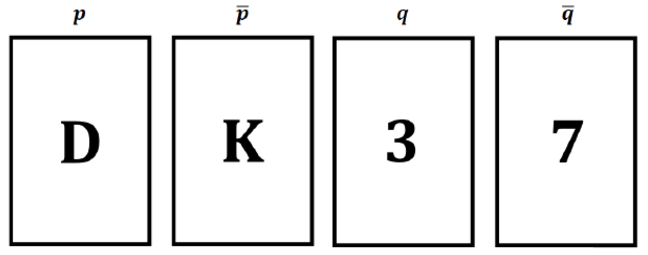
\includegraphics[scale=0.5]{wasonAbstract}
\caption{The Abstract case of the Wason Selection Task}
\label{fig:wst}
\end{center}

\end{figure}

The Abstract case of the WST presents the subject with four cards on a table as shown in Figure~\ref{fig:wst}. Their face-up sides read $D, K, 3,$ and $7$. Participants are told that each card has a number on one side and a letter on the other. They are then asked which cards must be turned over to test the rule:

\begin{center}
``If there is a $D$ on one side of the card, then the other side shows $3$."
\end{center} 

\begin{table}
\begin{center}


\begin{tabular}{ c c c}
  \textbf{$D$}&  \textbf{$3$}& \textbf{$(3\leftarrow D)$} \\ 
  \hline
 $\top$ & $\top$ & $\top$\\  
 $\top$ & $\bot$ & $\bot$\\  
 $\bot$ & $\top$ & $\top$\\
 $\bot$ & $\bot$ & $\top$
\end{tabular}
\caption{Propositional evaluation of the implication $3 \leftarrow D$ for each possible truth value of $3$ and $D$.}
\label{tbl:wst_impl}
\end{center}
\end{table}

\begin{table}
\begin{center}


\begin{tabular}{ c c c}
  \textbf{$D$}&  \textbf{$3$}& \textbf{$(3|D)$} \\ 
  \hline
 $\top$ & $\top$ & verification\\  
  $\top$ & $u$ & non-applicability\\ 
 $\top$ & $\bot$ & falsification\\  
 $\bot$ & $\cdot$ & non-applicability\\
 $u$ & $\cdot$ & non-applicability
\end{tabular}
\caption{De-finetti evaluation of the conditional $(3|D)$ for each possible truth value of $3$ and $D$.}
\label{tbl:wst_classical}
\end{center}
\end{table}

\begin{figure}
\centering 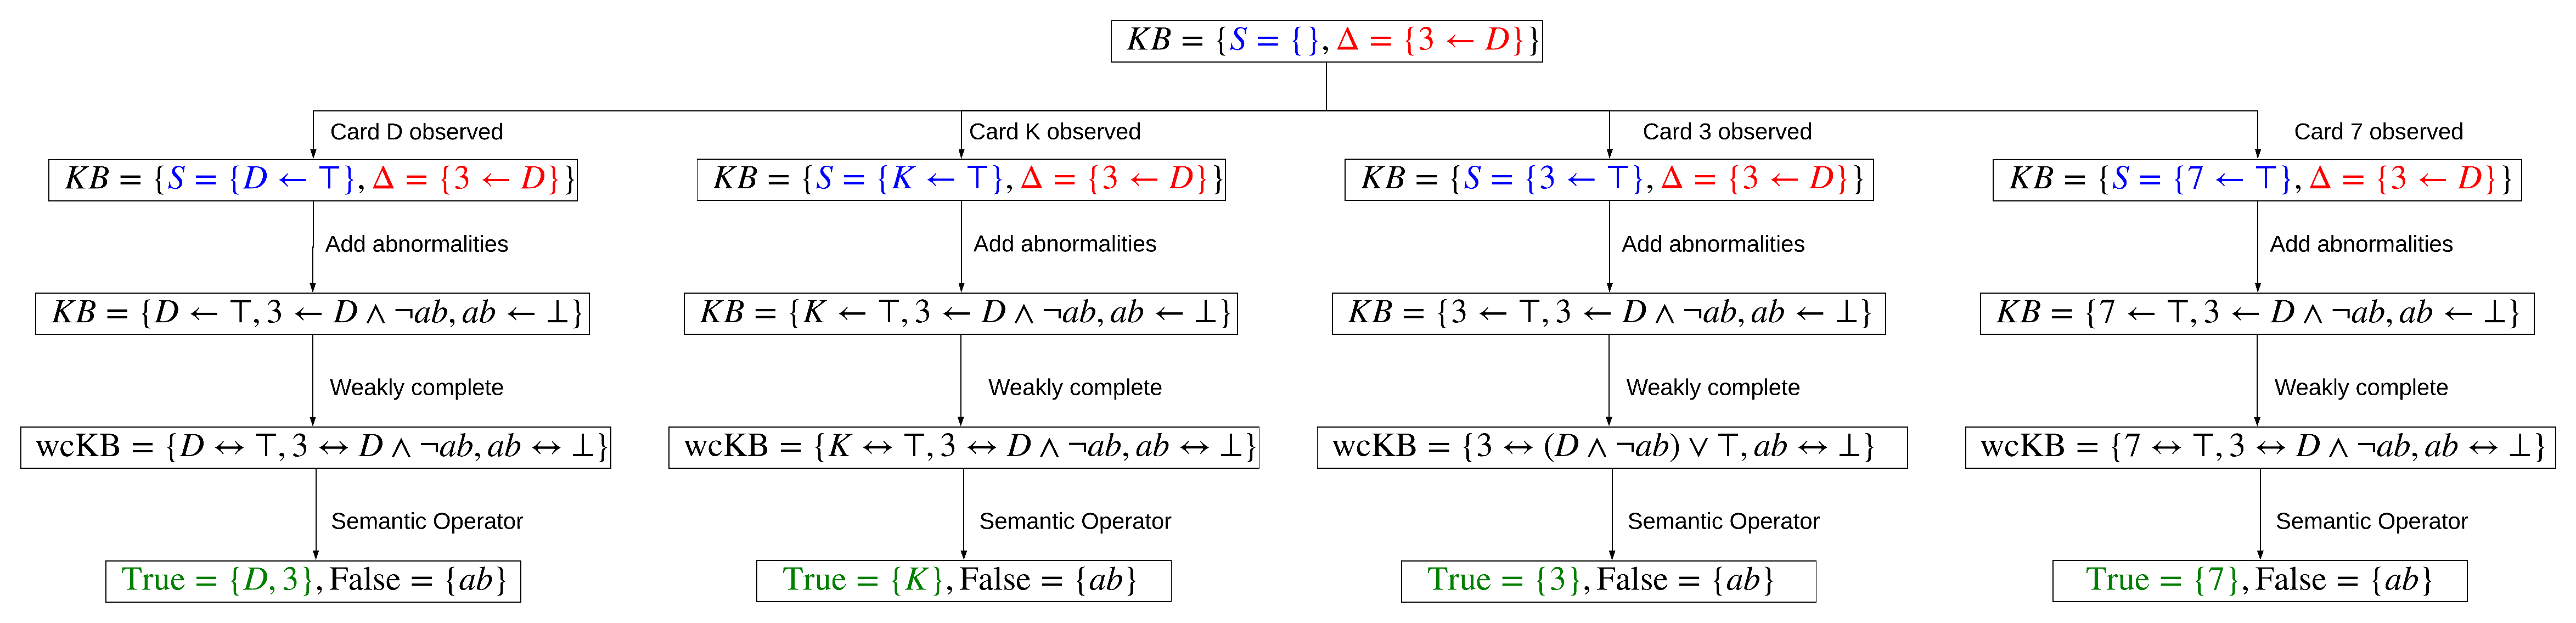
\includegraphics[width=\linewidth]{WST_WCS}
\caption{Application of the WCS to the abstract case of the WST for the basic weak completion approach.}
\label{wst_wcs}
\end{figure}

This task requires the participants to find possible defeaters for the conditional rule. Assuming the \textit{de Finetti} truth table from Section~\ref{ssec:condi} for the interpretation of conditionals of the form ``If $\psi$ then $\phi$", Table~\ref{tbl:wst_impl} shows that the cards pairs $(D,3)$ and $(D,7)$ are both possible defeaters to the rule $(3 \leftarrow D)$ because the rule $(3|D)$ is only verified or falsified when the interpretation maps $(D,\top)$ and $(3, \lnot u)$. Any observed card which allows a possible world with both of those assignments is a possible defeater. If a participant were to turn the $D$ card and find a number that was not $3$, or were to a turn the card $7$ and find the letter $D$ on the other side, the classical interpretation of conditional would not hold. Thus these two cards must be turned to check the rule. However, human subjects very seldom choose this classical answer set and instead overwhelmingly prefer to turn the cards $D$ and $3$. Table~\ref{tbl:can} shows the most common card selection sets for participants.

A great many cognitive theories have been applied to these results, with varying degrees of success \citep{ragni2017formal}. This paper will focus on the WCS interpretation of the task provided by \cite{ragni2017wason}. This approach assumed an initial knowledge base $\text{KB}$ containing only the conditional $(3|D)$ and an interpretation of the conditional as a license for implication.

\cite{dietz2012computational} showed that the abstract case of the WST could be modelled using the WCS and 3-valued \L ukasiewicz logic. Using the conditional as the initial logic program, we write $\text{KB}=(S=\{\},\Delta=(3|D))$. Treating conditionals as licenses for implication, $\text{KB}$ can be rewritten as $\text{KB}=\{3\leftarrow D \land \lnot \text{ab}_1\}$ where $\text{ab}_1$ is an abnormality predicate. Now $\textrm{lm wc}(\text{KB})=\top=\{\},\bot=\{ab\}$, and no information is obtained that could either verify or falsify the conditional. In order to adapt the WCS to the WST they introduced the concept of observation support.

\begin{table}
\begin{center}


\begin{tabular}{ c c c c }
  \textbf{Observation $O$}&  \textbf{Explanation $\epsilon$}&\textbf{$\text{lm wc (KB}\cup \epsilon)$}& \textbf{Turn Function} \\ 
  \hline
 $D$ & $\{D\leftarrow \top\}$ & $\{D,3\}\{\text{ab}_1\}$&turn\\  
 $K$ & $\{K\leftarrow \top\}$ & $\{K\}\{\text{ab}_1\}$&do not turn\\  
 $3$ & $\{D\leftarrow\top\}$ &$\{D,3\}\{\text{ab}_1\}$&turn\\
 $7$ & $\{7 \leftarrow \top\}$ & $\{7\}\{\text{ab}_1\}$&do not turn
\end{tabular}
\caption{Dietz' computational logic approach to the abstract case of the WST.}
\label{tbl:wst_lmwc}
\end{center}
\end{table}

The set of abducibles $A$ corresponds to positive and negative facts which are not assigned in $\text{KB}$. For the WST as formulated here $A=\{D\leftarrow \top,D\leftarrow \bot,3\leftarrow \top,3\leftarrow \bot,K\leftarrow \top,K\leftarrow \bot,7\leftarrow \top,7\leftarrow \bot\}$.
 An observation $O$ is \textit{explained} by a minimal explanation $\epsilon \in A$ if and only if $O$ holds in $\textrm{lm wc}(KB\cup\epsilon)$. Table~\ref{tbl:wst_lmwc} shows the least models that can be drawn for the observations $D$, $3$, $K$, and $7$. If a least model obtained in this way contains atoms and atomic assignments that could verify or falsify the conditional (i.e. make $I_{\textrm{lm wc}(\text{KB}\cup \epsilon)}(3|D)\neq$ non-applicability when using the \textit{de Finetti} truth table), then the observed card should be turned. Figure~\ref{wst_wcs} shows the derivation of $\textrm{lm wc}(\text{KB}\cup \epsilon)$ for $\epsilon=D, \epsilon=3, \epsilon=K$, and $\epsilon=7$.\footnote{This approach differs in description from the author's original one, in which a card was turned if the least model assigned non-$u$ values to every variable in the conditional (i.e. $3$ and $D$), but is identical in practice.}


This simple interpretation of the WST which applies abduction to the initial knowledge base to derive the observation is sufficient to model the general reasoner. It does not, however, explain any of the other deviant cases which are observed in Table~\ref{tbl:can}. Why, for example, should it be considered accurate if it gives no information about the classically accurate choice of the $D$ and $7$ cards, chosen by 19 participants, a significant proportion? Instead, consider how these aberrant reasoners could be modelled. Perhaps they use extra computational steps or omit steps? This author has previously shown that the WCS is able to model these individual reasoners \citep{breu2019weak}\footnote{My contribution to this paper was the initial proposal of the extensions, their integration, the silencing mechanism used for modelling individual reasoners, and the broad idea of the stochastic evaluation technique itself.} by including three simple processes: \textit{basic weak completion}, \textit{abduction} (as we have already discussed in this section), and \textit{contraposition}. By including these three processes, and stochastically controlling when they are activated or silenced, it has been shown that not only is this extended framework able to model the major cases of the WCS, but very close approximations to empirical frequency results can also be drawn for all three cases of the WST (Table~\ref{tbl:can_full}).

\subsubsection*{Basic Weak Completion}

Basic weak completion ignores the existence of other least models which may validate or invalidate the inference $(3|D)$ and, instead handles only those cases where $\epsilon \leftrightarrow (O\leftarrow \top)$. That is, only information about the currently observed card is considered in the abductive framework. Figure~\ref{wst_wcs} illustrates this process for each of the four observations: $D$, $3$, $K$, and $7$. Now only $\textrm{wc lm}(KB \cup (D \leftarrow \top))$ provides assignments which for which the de Finetti interpretation of $(3|D)\neq \textrm{non-applicability}$. Observing the card $3$ no longer leads to the decision to turn the card because only the case $\epsilon = (3\leftarrow \top)$ is considered and the case $\epsilon = (D \leftarrow \top)$ is not considered.

\subsubsection*{Contraposition}
\begin{table}
\begin{center}
\begin{tabular}{ c c c }
 \textbf{Iteration} & \textbf{$\top$} & \textbf{$\bot$} \\ 
 \hline
 0 &  &  \\  
 1 &  $7$ & $ab_1$, $ab_2$  \\  
 2 &  $7$ & $3$, $ab_1$, $ab_2$  \\
 3 &  $7$, $D'$ & $3$, $ab_1$, $ab_2$  \\
 4 &  $7$, $D'$ & $3$, $ab_1$, $ab_2$, $D$  
\end{tabular}
\caption{Applying the Weak Completion Semantics and Contraposition to the $7$ card of the WST.}
\label{tbl:7cont}
\end{center}
\end{table}

Contraposition implicitly makes use of \textit{modus tolens}, usually assumed to be silenced in human cognition, to derive certain canonical cases in the WST. Using contraposition it becomes possible to model individual participants who choose to turn the cards $D$ and $7$ (the classical response).

Contraposition is applied as follows for the initial knowledge base $KB$:
\begin{enumerate}
\item For each conditional $(\psi|\phi)\in KB'$ :
\begin{itemize}
\item Add the conditional $(\phi'|X)$ to $\Delta$, where $X$ is the other possible value for that card face\footnote{$(D,K),(3,7)$}.
\item Add the fact $\phi\leftarrow \lnot \phi'$ to $S$.
\end{itemize}
\item Interpret conditionals as licenses for implication.
\item Apply the Abductive case of the WCS as normal.
\item Turn the card if and only if some or $I_{\text{lm WC (KB} \cup \epsilon)}(\psi|\phi)\neq\textrm{non-applicability}$ or some $I_{\text{lm WC (KB} \cup \epsilon)}(\phi'|X)\neq\textrm{non-applicability}$, and $\text{lm WC (KB} \cup \epsilon)$ explains $O$.
\end{enumerate}

Using this technique, and applying basic weak completion (i.e. only considering the case $\epsilon\leftrightarrow(O\leftarrow \top)$ it is possible to model the classical case of the WST. The resolution for the $7$ card is as follows:

\[
KB = (S=\{\},\Delta=\{(3|D)\})
\]
\[
KB' = (S=\{D \leftarrow  \lnot D'\},\Delta\{=(3|D),(D'|7)\})
\]
\[
KB' = \{3 \leftarrow D \land \lnot \text{ab}_1, D' \leftarrow 7 \land \lnot \text{ab}_2, \text{ab}_1 \leftarrow \bot, \text{ab}_2 \leftarrow \bot\}\}
\]
\[
KB'\cup (7\leftarrow\top) = \{3 \leftarrow D \land \lnot \text{ab}_1, D' \leftarrow 7 \land \lnot \text{ab}_2, \text{ab}_1 \leftarrow \bot, \text{ab}_2 \leftarrow \bot, 7 \leftarrow \top\}\}
\]
\[
\text{wc}KB'\cup (7\leftarrow\top) = \{3 \leftrightarrow D \land \lnot \text{ab}_1, D' \leftrightarrow 7 \land \lnot \text{ab}_2, \text{ab}_1 \leftrightarrow \bot, \text{ab}_2 \leftrightarrow \bot, 7 \leftrightarrow \top\}\}
\]
\begin{equation} \label{eqn:wst_contra}
\textrm{wc} (KB'\cup (7\leftarrow\top)) = \{3 \leftrightarrow D \land \lnot ab_1, D' \leftrightarrow (\lnot 3 \land ab_2) \lor (\lnot D),  ab_2\leftrightarrow \bot, ab_1\leftrightarrow \bot, 7\leftrightarrow\top \}
\end{equation}

Table~\ref{tbl:7cont} shows the computation of $\textrm{lm wc} (KB'\cup (7\leftarrow\top))$. From this, it is possible to deduce that the card $7$ must be turned. Figure~\ref{fig:wstcano} illustrates the use of these extensions to derive all four of the canonical cases of the WST.

 
\subsubsection*{Combined Model}
By combining our contraposition and abductive models for inferences, it is possible to model the case where the cards $D$, $3$, and $7$ are turned. Combining the models $(A_i,...,A_n)$ is done by turning a card $c$ if and only if $c$ would be turned in some model $A_i$.

This work has shown that all canonical cases of the weak completion semantics can be modelled by activating or silencing these three processes on the initial knowledge base. The intuition that a discrete and systematic succession of well-founded processes could be used to model multiple different results for the same experiment was the inspiration for the SCP framework which this thesis introduces.


\begin{figure}
\centering 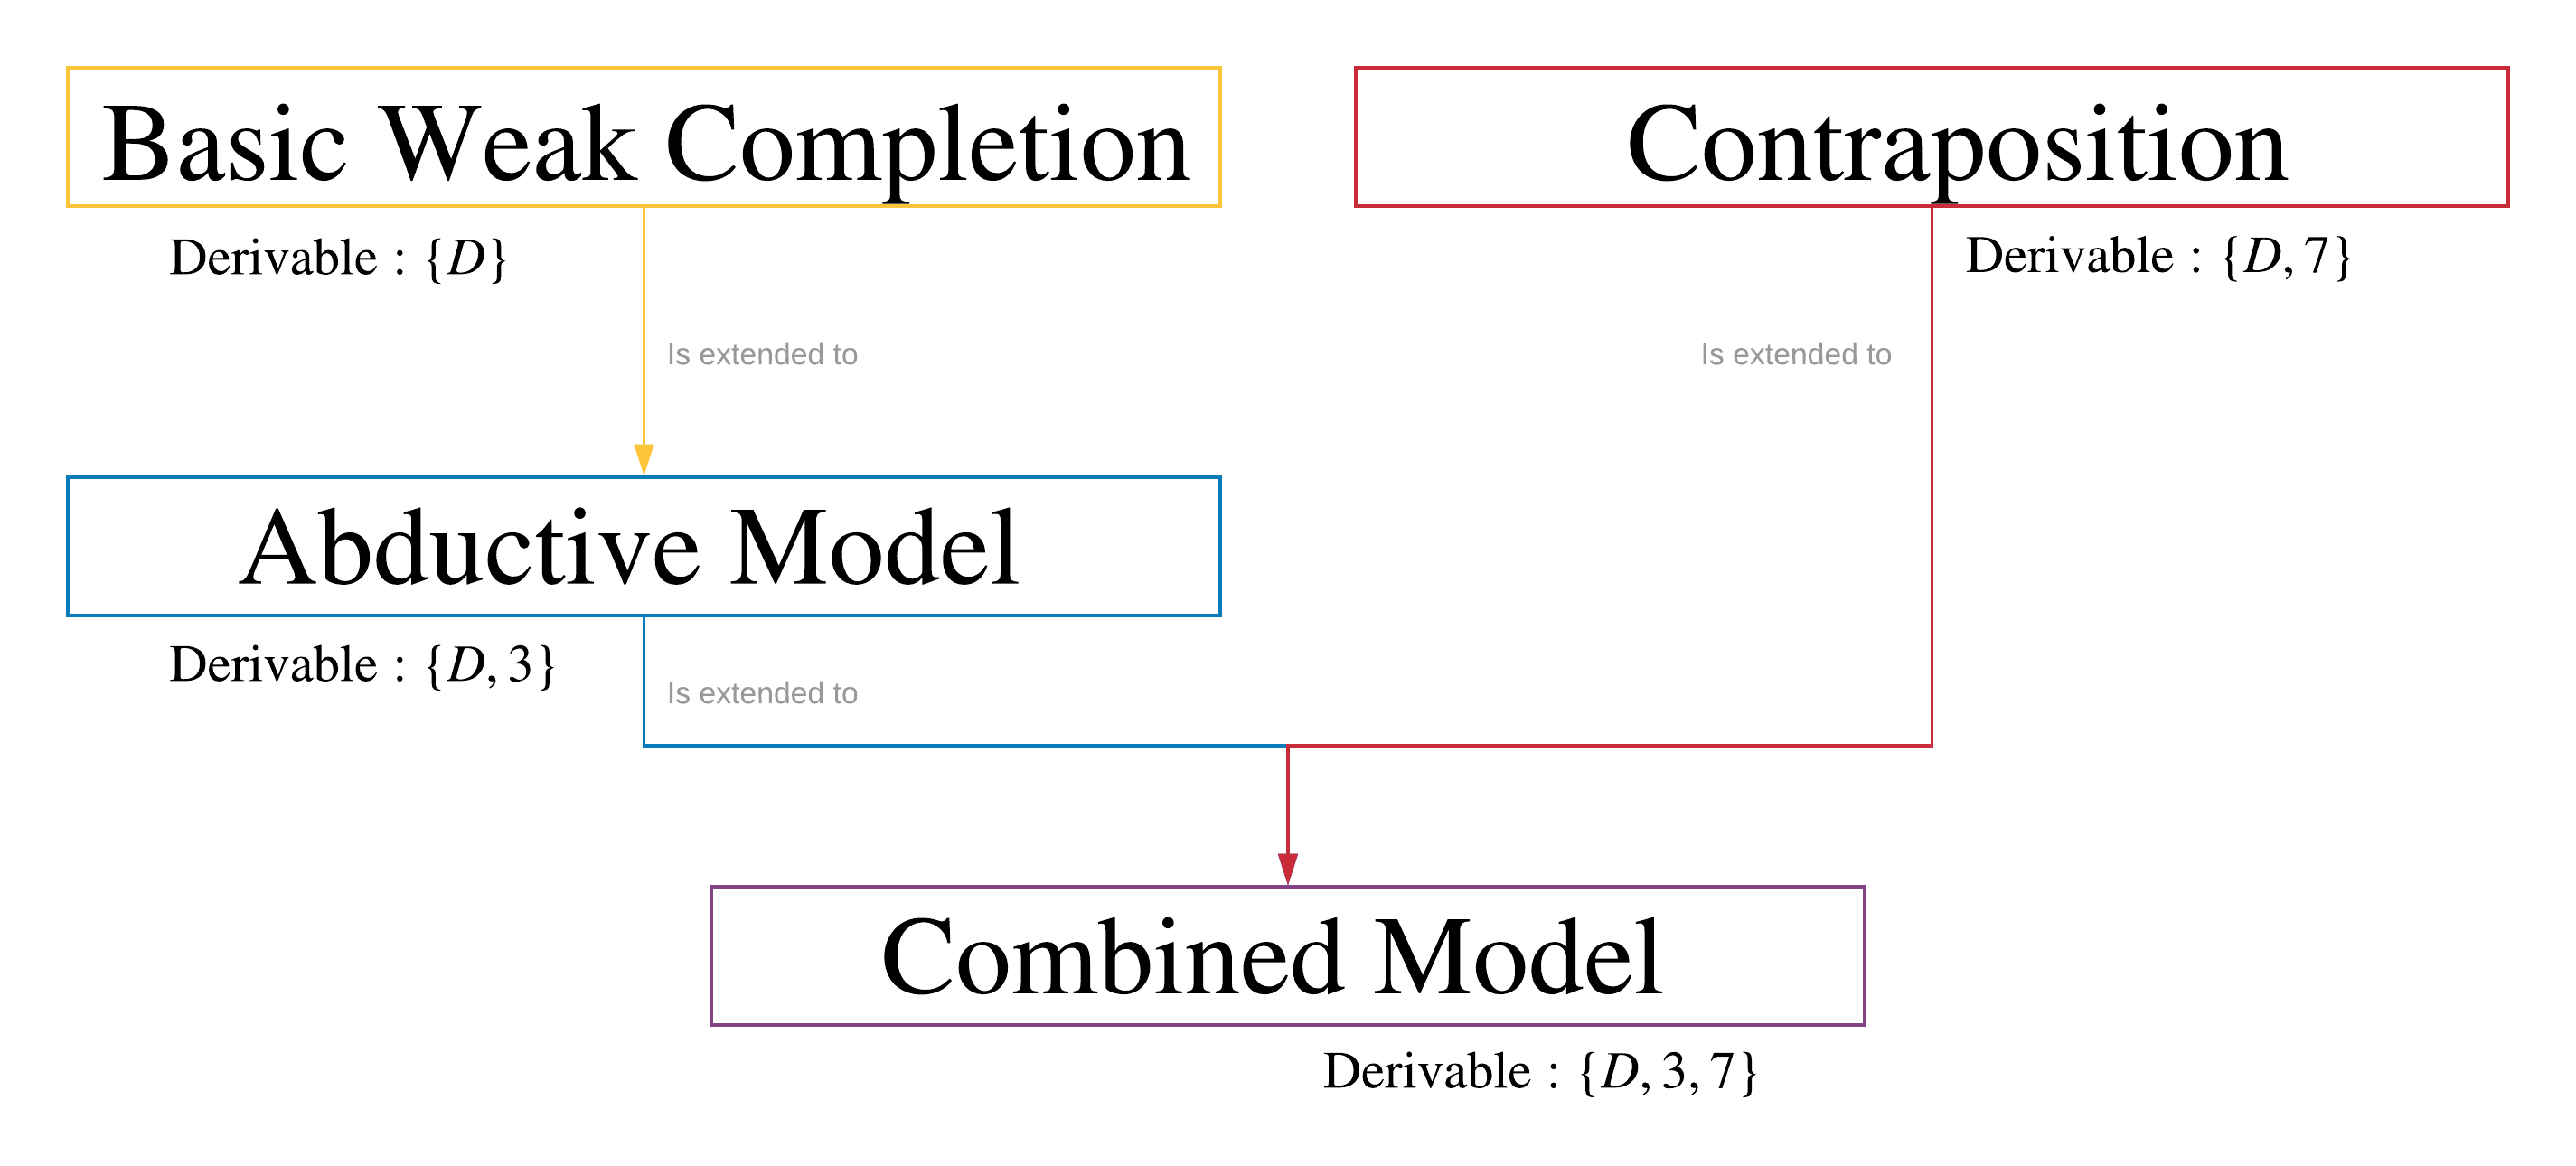
\includegraphics[scale=.6]{wst_cano}
\caption{Using the abduction and contraposition extensions to derive all four canonical cases. Arrows indicate that the origin model produces a subset of the turn instructions of the endpoint.}
\label{fig:wstcano}
\end{figure}





















\chapter{Sequential Cognition Processes} \label{chp:scp}
\section{SCPs: An Intuitionist Description} \label{ssec:intu}
\begin{figure*}
\begin{subfigure}{.35\textwidth}
  \centering
  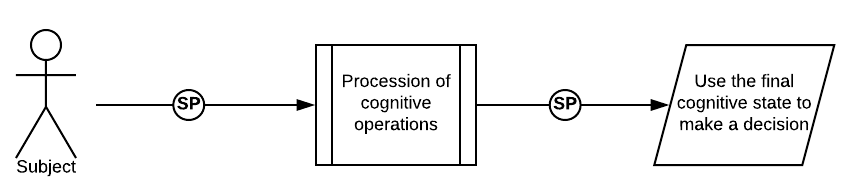
\includegraphics[width=0.97\linewidth]{general}
  \caption{Unrestricted SCP.}
  \label{fig:scp_general}
\end{subfigure}%
\begin{subfigure}{.65\textwidth}
  \centering
  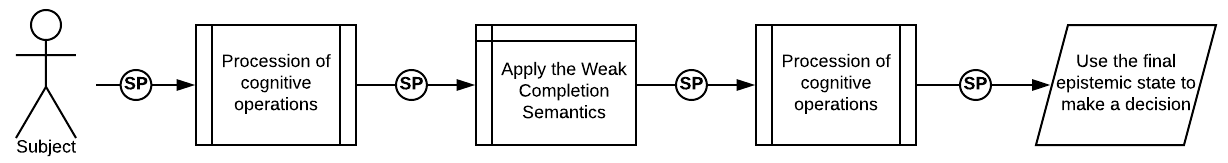
\includegraphics[width=0.97\linewidth]{generalWCS}
  \caption{WCS guaranteed to occur.}
  \label{fig:sfig2}
\end{subfigure}
\caption{The most general description on an SCP with and without guaranteeing the WCS is applied at least once. An agent transitions from one epistemic state to another and then uses it to make a decision. $SP$ nodes indicate state points.}
\label{fig:scp_generalWCS}
\end{figure*}

Although there is evidence that the brain can perform several simultaneous operations when considering a task (such as when considering an image \citep{sigman2008brain}, the SCP framework assumes that at some points in reasoning about a given task, the mental processes of the agent converge to a set of epistemic states, called a \textit{state point}. Whatever happens between these points of convergence can contain any number of parallel processes. The collection of processes that occur between any two state points in a reasoning task is called a \textit{cognitive operation}. It follows that any cognitive operation is valid as long it takes a set of epistemic states as input and produces a set of epistemic states as output. Figure~\ref{fig:scp_general} outlines an SCP-like structure that is powerful enough to model any cognitive task that involves an epistemic state transition. However, it does not provide any useful information; the nature of the processes followed is completely undescribed. Suppose, instead, that some cognitive task is being modelled, and that researchers have reason to believe that The Weak Completion Semantics should play a part in their model. Under this new restriction, and assuming a sufficiently expressive epistemic state, Figure~\ref{fig:scp_general} is still an accurate model of the process, but now so is Figure~\ref{fig:sfig2}. By sacrificing some of the ambiguity -- and, thus, expressiveness -- of the model, the information content of the model description has increased. This trade-off is a feature of the SCP framework and finding the right depth of complexity to model the task accurately and still provide meaningful information is more art than science at present. 

\section{SCPs: Mathematical Formulation}
An SCP Task $\Pi=(s_i, M, f(), \gamma)$ consists of an initial epistemic state $s_i$, a known set of cognitive operations $M$, a desired final output $\gamma$, and an external function $f()$ which generates those final outputs by translating the final epistemic state into an empirically grounded set of possible responses. An epistemic state $s_k$ describes all the information available to the agent at state point $k$. The precise contents of an epistemic state should be chosen so that at least some $m \in M$ are able to accept that state as an input. In the case of a system containing only the one complex operation which applies the WCS, one possible epistemic state is $s=(P,\Delta,V)$, where $P$ is a set of inference rules of the form $(head \leftarrow body)$, $\Delta$ is a set of conditional rules of the form $(\psi|\phi)$ and $V$ is a mapping of atom names appearing in $KB$ to a truth value in \L ukasiewicz logic ($\top,u, \bot$). In principle this definition will serve for the rest of the paper, but it is extended slightly so that $s_k = (S,\Delta,V,R)$ where $R$ is a set of labelled categorization criteria sets (\textit{LCS}). An LCS $ c \in R$ consists of a category name and list of rules and atoms which fit into that category.

A base point is a single epistemic state. A state point $p$ is defined recursively by $p=\{\bar{p} \oplus Q \}$ where $\bar{p}$ is a base point, and $Q$ is a set of state points, and $\oplus$ represents the exclusive-or operation\footnote{$(X \oplus Y) = ((X \cup Y) - (X \cap Y))$ for sets $X$ and $Y$.}. State point containment $\in_s$ for state points $p$ and $q$ is defined recursively as follows:

\[
p \in_s q = \begin{pmatrix} p \in q  & \textrm{True} \\   \exists_{r\in p}p \in_s r = \textrm{True} & \textrm{True}   \\ \textrm{Otherwise} & \textrm{False} \end{pmatrix}
\]

It is never the case that $p \in_s p$.

A cognitive operation $m = (\chi, e), m \in M$ consists of a precondition $\chi$ and a process $e$, such that for an input state point $p$, every base point $\bar{p} \in_s p$ is either accepted as input ($\bar{p} \models m[\chi]$ under whatever definition of $\models$ is used for the complex operation $m$), or else rejected. Every base point is evaluated by the complex operation in isolation (no other base point $\bar{q}$ can affect the output of $m$ on base point $\bar{p}$).

$J[\bar{p},m]=p'$ describes the \textit{application} of a base point $\bar{p}$ to a cognitive operation $m \in M$ to produce an output base point $p'$, where $p'$ is vector of base points. $p'$ is \textit{defined} if and only if $\bar{p}$ is a valid input for $m$ (Section~@TODOsection). In this way, a single single base point may produce multiple base points as output, reflecting potentially non-monotonic or non-deterministic properties of cognitive operations. 

We overload the functionality of $J$ so that $J[p,m]=p'$, where $p$ is a state point (rather than just a base point), and define $J[p,m]$ as follows: $J[p,m]=[ \texttt{replace}(\bar{p} \in p,J[\bar{p},m])]$. $J[p,m]=p'$ is \textit{defined} if and only if some $J[\bar{p} \in p,m]$ is defined.

It follows that the depth of a state point is directly related to the number of complex operations which have been performed in the SCP prior to its occurrence. If a base point does not meet the precondition (see Section~@TODOref), it is either ignored completely and not processed (\textit{cruel application}), or passed exactly as is to the next complex operation (\textit{lenient application}). It is worth noting that the type of cognitive states produced as output by $m$ may not be the same as those of the input.
 
A cognitive operation is called monotonic if it always yields a base point as an output given a base point input ($J[\bar{p},m]=\bar{p'}$).

This paper will focus on cases where the type of cognitive state remains constant, but it is possible for $J[\bar{p},m]=p'$ where $\bar{p}$ is of structure $(\alpha,\beta)$ and $\bar{p'}\in p'$ to be of structure $(\alpha,\beta,\gamma)$ @TODOdefiniestrcutureinepis. Future models of human cognition may well rely on background knowledge which draws inferences from multiple types of non-monotonic logics.

A cognitive transition model (\textit{CTM}) describes an ordered procession of cognitive operations following an initial epistemic state as follows: CTM $\pi=(s_i\longmapsto m_1\longmapsto ...\longmapsto m_n)$ where $s_i$ is a state point, and $m_k$ is a cognitive operation. A partial cognitive transition model (\textit{pCTM}) $\pi=(m_1\longmapsto ...\longmapsto m_n)$ describes a procession of cognitive operations without an an initial state point.

The CTM $\pi = (s_i\longmapsto m_1 \longmapsto ...\longmapsto m_n)$, for SCP task $\Pi=(s_i, M, f(), \gamma)$ is \textit{defined} if and only if $J[p_k,m_k]$ is defined for $p_k = J[p_{k-1},m_k]$, $k>2$, and $J[s_i,m_1]$ is defined. The set of possible CTMs for SCP task $\Pi$ is given by $L[\Pi]=\{\pi\}$, where $\pi$ is a defined CTM for $\Pi$.

An SCP $\mu=(\pi,f())$  pairs a CTM $\pi$ with an external activation function $f()$ (Section~@TODOsection). An SCP $\mu=(\pi,f())$ is defined for SCP task $\Pi=(s_i, M, f(), \gamma$ if and only if $\pi \in L[\Pi]$.

---
@TODOmovetoValidity
An SCP is called \textit{credulously valid} if $f(\pi) \models \gamma$ for at least one epistemic state in the final state $p_n$. An SCP is called \textit{sceptically valid} if $f(\pi) \models \gamma$ for every epistemic state in the final state. In cases where all operations are monotonic, sceptical validity is the same as credulous validity.
---

Finally, we define a realised SCP $r = (k, f())$ where $k \in K[\pi]$, and $K[\pi]=\{s_i \longmapsto (m_1,\bar{p}_1) \longmapsto ... \longmapsto (m_n,\bar{p}_n)\}$ where, for every pair $(m_i,\bar{p}_i)$, $\bar{p}_i \in J[\bar{p}_{i-1},m_i]$. Realised SCPs describe a single agent's interpretation of an SCP and associate only a single epistemic state, rather than a state point to the output each cognitive operation in an SCP. 

$r=(k, f())$ is a realised SCP for SCP $\mu=(\pi,f())$, with $\pi=(s_i\longmapsto m_1 \longmapsto ...\longmapsto m_n)$ is given by $k=(s_i \longmapsto (m_i, \bar{p_1} \in J[\bar{p}_{0},m]) \longmapsto ... \longmapsto (m_n, \bar{p_n} \in J[\bar{p}_{n-1},m]))$.

When every cognitive operation in $M$ is monotonic, it is trivially easy to transform an SCP into a realised SCP and vice versa @TODOproof. In cases where SCPs are monotonic, we will use the SCP and its realised SCP interchangeably. The number of realised SCPs for an SCP is the same as the number of base points in the final state point of that SCP.



\section{SCP Tasks vs. SCPs vs. Realised SCPs}

SCP tasks describe a problem that needs to be solved and the limitations which the solution must to adhere to; SCPs describe a single 'recipe' that can be used to describe a sequence of well-founded, non-monotonic operations which an agent might use to model a problem; and realised SCPs describe how adherence to specific SCP can result in some agent coming to a conclusion that matches empirical data.

For a given SCP task there can be many possible SCPs (the question of how to choose the most probable of these candidate SCPs is discussed in Section~@TODOref), or no possible SCPs at all.

Figure~\ref{fig:scpExam} illustrates a situation in which students are asked if they will pass their next exam, and considers the example from the perspective of the SCPs task and associated variables, two possible SCPs describing different approaches to modelling the Task, and the Realised SCPs which could result. This figure is provided using propositional logic, and examples using non-monotonic logic will be introduced in Section~\ref{chp:experiments}.

\begin{figure}
\begin{center}
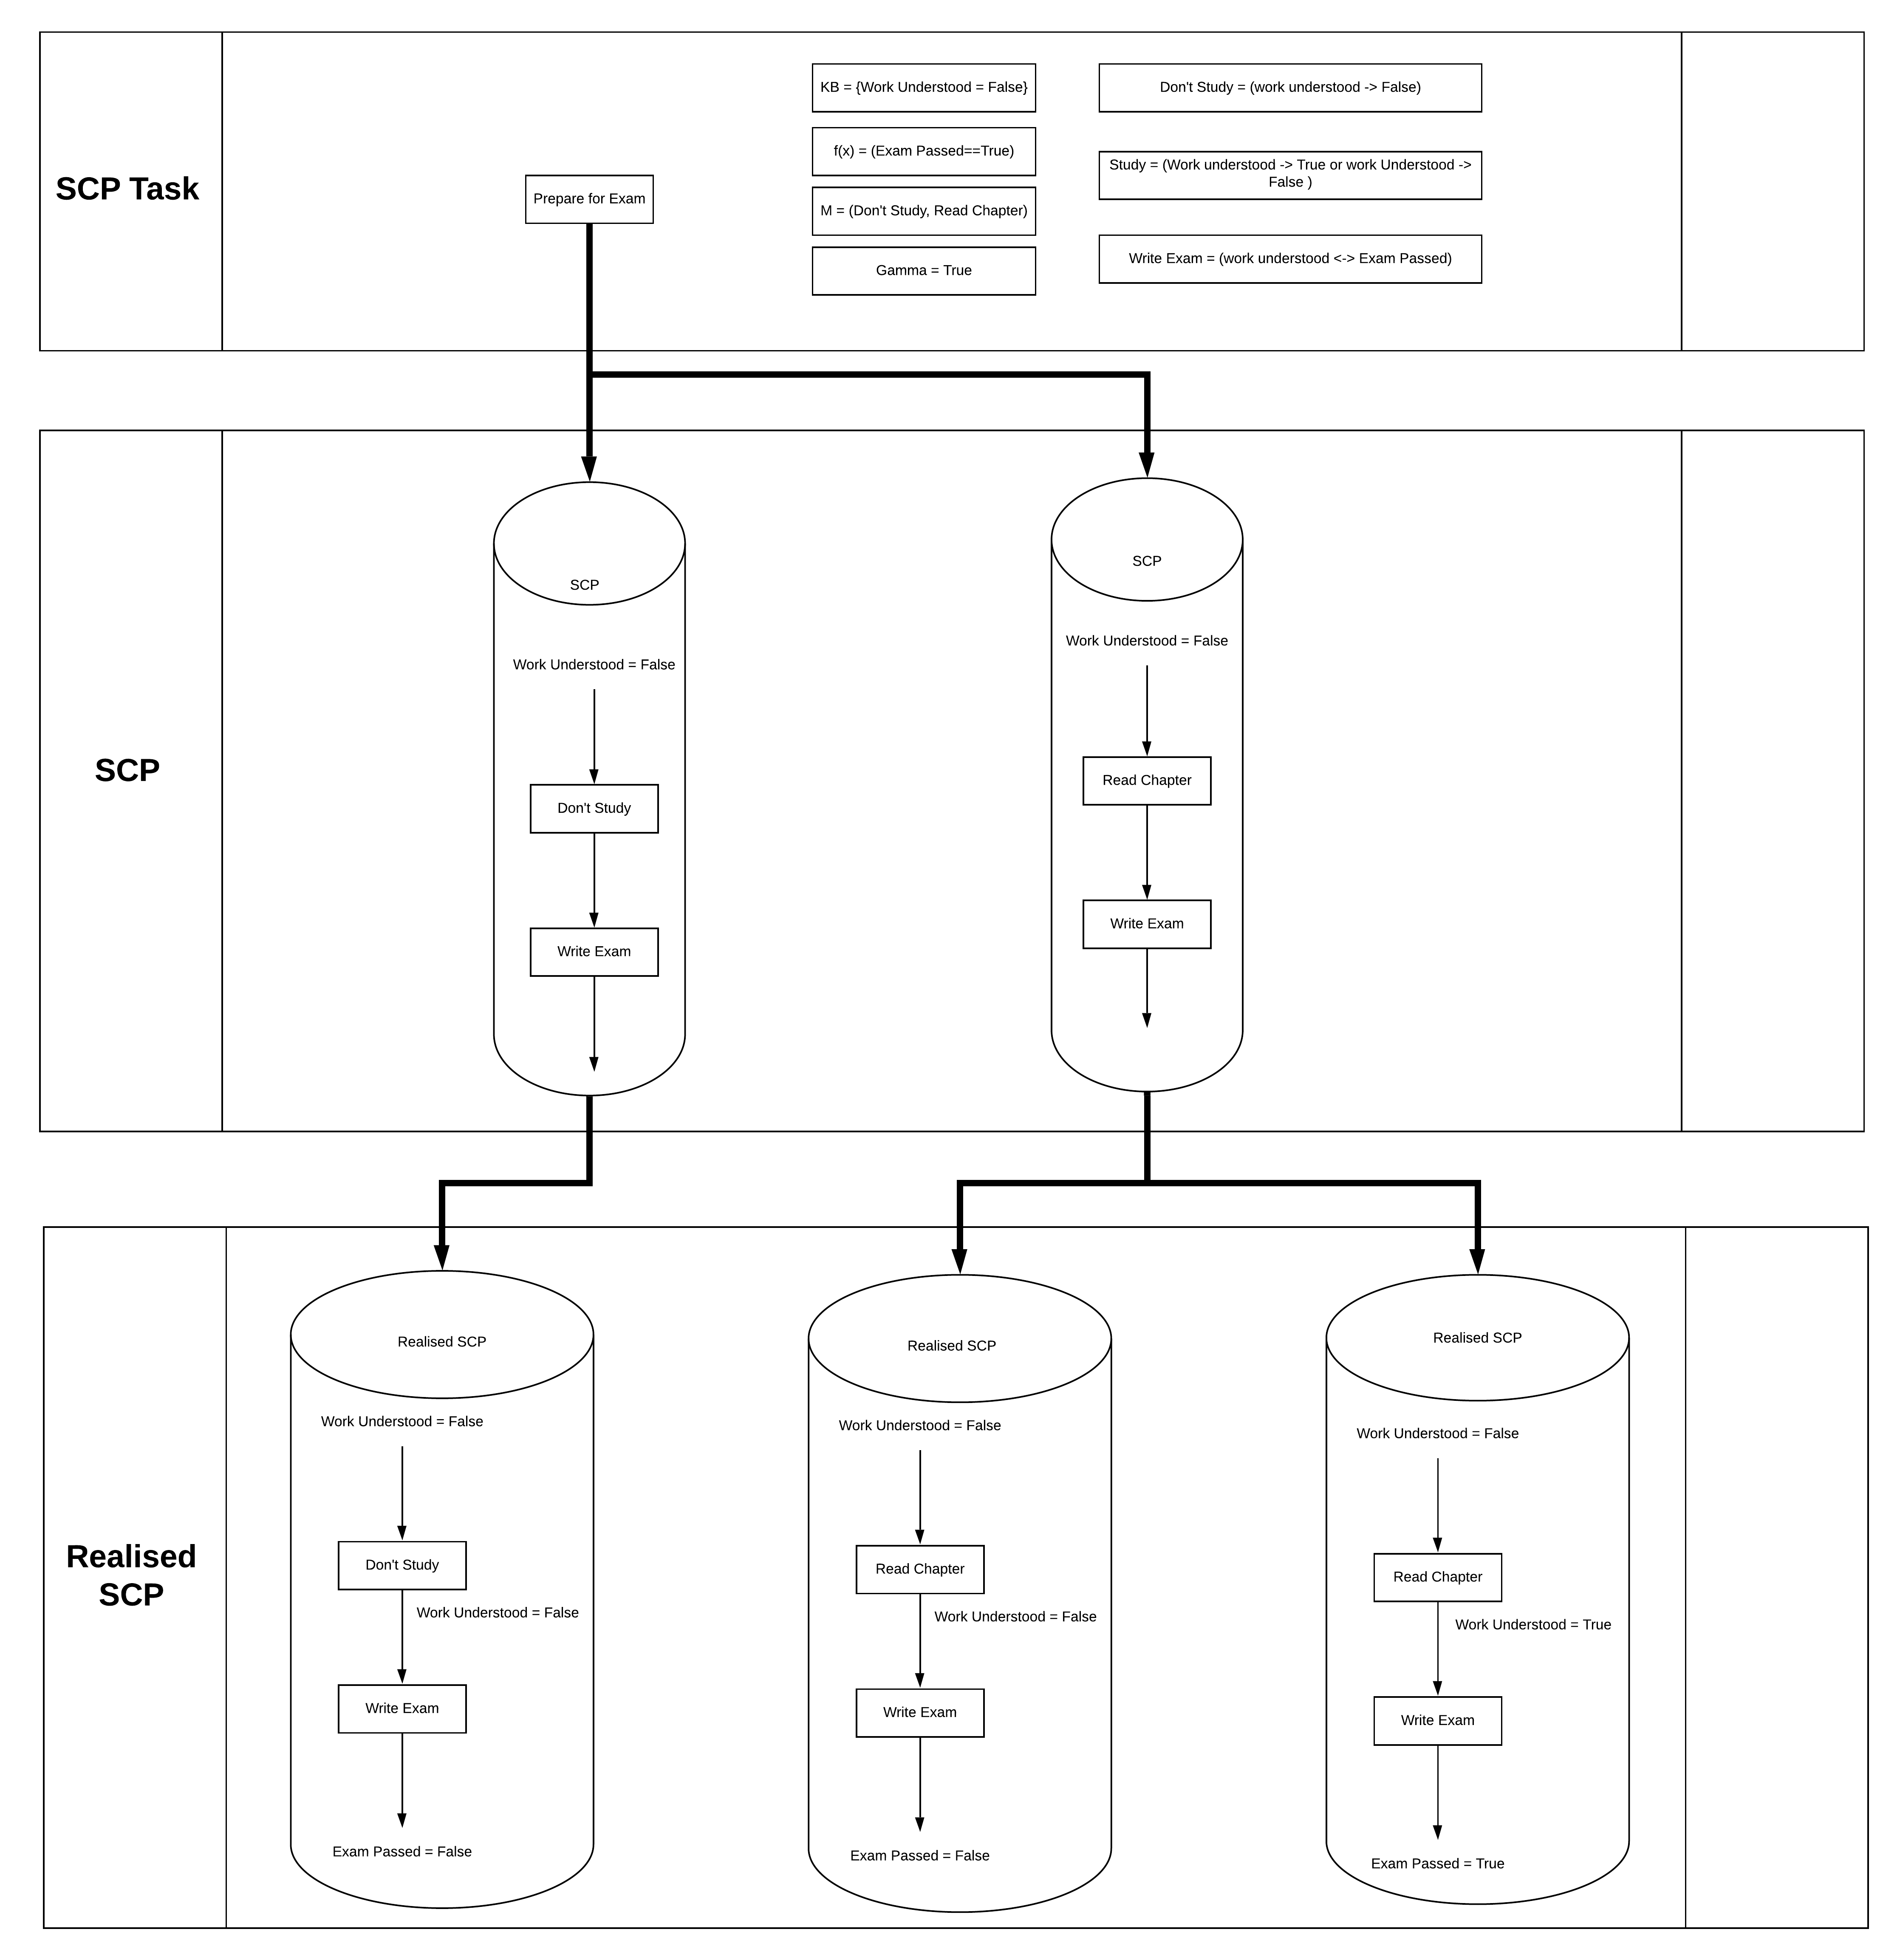
\includegraphics[scale=0.4]{ExamSCP}
\end{center}
\caption{An SCP Task, SCP, and Realised SCP describing whether a student will pass their exam. @TODOredodiagram}
\label{fig:scpExam}
\end{figure}

\section{Epistemic States}
The choice of epistemic state is dependent on the properties that are known or suspected to be true for the cognitive task as a whole. For example, a researcher working on drawing inferences using boolean Propositional Logic can be certain that any SCP they create should be expressive enough to pass a boolean knowledge base and possible world to a cognitive operation . Thus, it might suffice to simply define $s_i=(KB)$ where $KB$ is a set of propositional rules. By contrast, a researcher using the WCS requires a system capable of both communicating a set of rules to the next complex operation, and of describing the results of repeated applications of the semantic operator. It might seem intuitive to simply append a set of conditional rules $\Delta$ to the state used for the propositional case and to use a the semantic operator as an external function to evaluate the SCP. And, though this approach works for many examples, it makes it impossible to perform further processing in the SCP \textit{after} applying the semantic operator. What if the conclusion drawn was meant to form part of the background knowledge of another process? In practice using $s_k=(S,\Delta,V, R)$, where $V$ is a set of (variable name, value pairs) and $R$ is a categorization variable, seems able to model all aspects of the WCS, including information related to the least model. 

As yet, there are no definite rules for creating an epistemic state, but Albert Einstein's famous advice from 1950 still rings true: ``Everything should be made as simple as possible, but no simpler.'' The ideal epistemic state is one that enables every reasonable cognitive operation in $M$ that might help model the problem, without adding superfluous functionality that might render searching the SCP space infeasible.

\subsection{Common State Point Properties}
Though state points are largely unbounded in the information that they can contain and communicate, this thesis will restrict itself to epistemic state structures which carry intuition both from the underlying logics which they utilise, and from properties of search in the field of AI Planning (@TODOref).

\subsubsection*{The possible world: V}
The possible world variable $V$ encodes information about the current world state the agent believes itself to be in. As in Section~\ref{chp:prelim}, the possible world variable consists of a conjunction of variable pairs of the form $(\textrm{atom},\textrm{value}n\textrm{domain}_\textrm{atom})$, where $\textrm{atom}$ occurs only once. Unlike in a true possible world, not every there exist $\textrm{atom} \in Sigma$ which do not occur in $V$.

$V[\phi]$ returns the pair $(\phi,\textrm{value}) \in V$. An interpretation of formula $\phi$ using $V$, $I_v[\phi]$ occurs as with any possible world except that, when an atomic name $a$ which occurs in $\phi$ when $V[a]$ is undefined is given the default value of that language during computation ($u$ in $\L$@TODOname logic, and $\bot$ in propositional logic.). This is a necessity born of the fact that infinite space is required to explicitly store every possible variable name. The reason that $V$ is used throughout this thesis is threefold: it ensures that the possible world of the agent at any state of its cognition is always known; it allows inferences drawn using one logic to be utilised as background knowledge in another logic; and in practical implementation it can prevent recalculation of complex rules that have been preciously interpreted.

\subsubsection*{Propositional Rule Set: S}
The propositional rule set $S$ is defined precisely as the knowledge base was defined in Section~@TODOsection.

\subsubsection*{The set of conditionals: $\Delta$}
The set of conditionals $\Delta$ is defined precisely as in the conditional knowledge base in Section~@TODOsection.

\subsection{The Categorization Variable}
%@TODOreformulatefors_k=(s,v,delta,r)
The final property of a cognitive operation that needs to be discussed is how it is able to interact with the categorization variable $R$. Imagine a case drawn from \cite{saldanha2017weak} where the difference between creating abnormalities for obligate and factual conditionals is discussed. The intuition behind the authors' work can be summarised by saying that there are two different types of conditional statement, those that \textit{have to be} true, and those that are \textit{usually} true. If it rains $r$, I will normally take my umbrella $u$ (in the absence of something abnormal happening, like a plague of umbrella-stealing gnomes). This a statement that is usually true, but some things are definitely true. For example, when it rains, water has to fall out of the sky $s$. This is an essential property of rain, not subject to abnormalities. Thus one useful set of categorizations for researchers seeking cosmic knowledge of weather patterns may be: $R=\{obligate: \{u \leftarrow r\}, factual: \{s \leftarrow r\} \}$. With these labels we might then expect that the process followed by the operation $m \in M$ which creates abnormalities would treat the two conditionals in $KB$ differently, because of their assignments in $R$. $R$ then is a way of expressing meta information to the cognitive operations, and it is completely possible that some operation $m_k$ might change $R$ is such a way that future operation $m_{k+l}$ produces different output. This is a technique we will exploit in several examples in this paper.

@TODOdefinereachability
\section{Cognitive Operations}
The set of possible complex operations $M$ determines many attributes of the achievable final state point $p_n$. If every $m \in M$ is monotonic, then $p_n$ will be a base point. If some cognitive operation is computationally complex or produces a very large number of output state points, then search using that base point becomes less efficient. If some complex operation $m'$ (such as weakly completing) is known or believed to occur in the SCP, then a restriction on the cognitive states exists such that either the initial state is of a format suitable as input for $m'$, or there exists another cognitive operation which is able to output a state point which contains base points of a suitable format.

More abstractly, the set of cognitive operations should be well-founded in the literature. The set of possible complex operations is infinite and an SCP only meaningfully describes human cognition when it contains cognitive operations that have been justified empirically (\textit{modus ponens-modus tolens} asymmetry, suppression, denial of the antecedent, etc.). 

\subsection{Pre-conditions and Effects} \label{ssec:precond}
The precondition $\chi$ of a cognitive operation $m$ refer to those conditions the input state point must satisfy in order for that operation to be considered valid. An SCP is valid if and only if every cognitive operation it contains is valid. For example, one might have a cognitive process describing Julie's plans for a night out on the town. Let us imagine that the SCP task describing her night out includes the operation \texttt{goHomeByCar}. Semantically, this operation should take her \textit{isHome} variable and set it to True.

The situations in which \texttt{goHomeByCar} can reasonably occur in an SCP are at the researchers' discretion. Researcher~1 might feel that it can be allowed at any point in the SCP and will simply have no effect for those input epistemic states in which she is already at home. Researcher~2 might argue that \texttt{goHomeByCar} is applicable only when \textit{isHome}=False. Researcher~3 knows that only the cognitive operation \texttt{goToClub} changes the \textit{isHome} variable, and so argues that \textit{isHome} is only applicable after \texttt{goToClub} occurs. There are merits to the arguments of each researcher.

Researcher~1 argues for a property called \textit{trivial validity}, that is that SCPs should always be considered valid, without any need for evaluation. This approach, however has one significant drawback: it cannot handle changes in the structure of epistemic state inputs. Imagine an epistemic operation called \texttt{dontDriveDrunk} which corresponds to our party animal realising that she shouldn't drive home of she's been drinking. Imagine further that this operation takes base points which are either of propositional or default structure (@TODOrefsection) and outputs an epistemic state of default structure which contains the new rule. If \texttt{goHomeByCar} took only a propositional state as input, then any sequence where \texttt{dontDriveDrunk} occurs as the previous operation will cause the SCP to fail because of the input state is not of an allowed type. Trivial validity then, is not sufficient for modelling SCP which state structure changes.

Researcher~2 has opted for a \textit{variable validity} approach. She has reasoned, correctly, that the \texttt{goHomeByCar} only results in an epistemic state change when when \textit{isHome} is not True. She therefore, feels that it only makes sense to reduce redundancy and search complexity in creating the SCP by only allowing the action to occur when it can be said to have an effect. This argument has some merit from an intuitive perspective, but presents an unpleasant question: what if there are state points in which only some ground points actually meet the precondition? To compound the troubles with this variable state approach to preconditions is the fact that it is not possible to determine SCP validity without evaluating the SCP at runtime, which could be slow for large SCPs.

Researcher~3 has taken an \textit{operator validity} approach, instead has focused on the structure of the SCP. This approach allows SCP validity to be determined without explicitly evaluating an SCP, one need simply search through the cognitive operations in the SCP to make sure that no operation has a precondition operation which has not yet occurred. This approach also presents drawbacks, it requires explicit knowledge of operation interactions, and adding a new cognitive operation to $M$ in the SCP Task might force several other operations to update or change their interactions. Further, there might be other cognitive operations which mean that the precondition operation is no longer in effect. Imagine a third operation \texttt{goHomeByTrain} which also sets \textit{isHome} to True. Now the sequence of operations $x\longmapsto \texttt{goToClub} \longmapsto \texttt{goHomeByTrain} \longmapsto \texttt{goHomeByCar}$ would still be valid with Researcher 2's original requirement that  \texttt{goToClub} occurred previously in SCP. However, it is obvious that \texttt{goHomeByTrain} has negated the effect of \texttt{goToClub}. Evidently this approach is not appropriate in any case in which other operations can silence the effect of those operations mentioned in preconditions.

Every approach has shows strengths and weaknesses, a final approach to consider is the \textit{hybrid validity} approach. With this approach, all cognitive operations are assumed to be valid, provided that the output base points of the previous operation are of a suitable input type for the current operation. Hybrid validity is an appropriate approach for all SCPs in which every cognitive operation has a known output structure. Though hybrid validity does not have the best-case search properties of the other approached, its universal validity means that it should generally be the starting point for generating SCPs. The hybrid approach is followed implicitly throughout the rest of this thesis and preconditions are omitted.

\subsection{Optimality, Satisfaction, Validity} \label{ssec:validity}
\subsubsection{Validity}
As discussed in Section~\ref{ssec:precond} validity can be defined for a cognitive operation and its input. Reaslied SCPs describe both the operation and the input for an SCP and allow us to define SCP validity as follows:

%generated from SCP $(\pi=(s_i \longmapsto m_1 \longmapsto ... \longmapsto m_n), f())$ was in here
A realised SCP $r=(k \in K[\pi],f())$, $k=(s_i \longmapsto (m_1,s_1) \longmapsto ... \longmapsto (m_n,s_n))$ with evaluation function $f()$ is valid iff $s_i$ is an epistemic state, every $m \in \pi$ is valid (according the validity requirements defined by the researcher), and $f(k)$ is defined. 

@TODOredefineKinFirstappearance

An SCP $(\pi,f())$ is valid if and only if there exists some realised SCP $r=(k \in K[\pi],f())$ which is valid.

An SCP Task $\Pi=(s+i, M, \gamma, f())$ is valid if and only if there exists some SCP $((\pi,f())$, with $(\pi=(s_i \longmapsto m_1 \in M \longmapsto ... \longmapsto m_n \in M)$ which is valid.

Validity does not require that $f(\pi)=\gamma$, only that external function $f()$ is able to make some prediction or set of predictions based $\pi$.


\subsubsection{Satisfaction} 

%generated from SCP $(\pi=(s_i \longmapsto m_1 \longmapsto ... \longmapsto m_n), f())$ was in here
A realised SCP $r=(k \in K[\pi],f())$, $k=(s_i \longmapsto (m_1,s_1) \longmapsto ... \longmapsto (m_n,s_n))$ with evaluation function $f()$ satisfies goal condition $\gamma$, written $r\models \gamma$ if and only if $r$ is valid, and $f(k)\models \gamma$. 

An SCP $(\pi,f())$ is satisfies $\gamma$, written $(\pi,f())\models \gamma$, if and only if there exists some realised SCP $r=(k \in K[\pi],f())$ for which $f(k)\models \gamma$.

An SCP Task $\Pi=(s+i, M, \gamma, f())$ is satisfies $\gamma$, written $\Pi\models \gamma$, if and only if there exists some SCP $((\pi,f())$, with $(\pi=(s_i \longmapsto m_1 \in M \longmapsto ... \longmapsto m_n \in M)$ which satisfies $\gamma$.

Heuristic Searches and machine learning techniques are generally used to find satisfying solutions for situations in which it is possible for an answer to be good enough for practical purposes. 

\subsubsection{Optimality}
Optimality refers to finding the best possible SCP to describe a problem according to whatever criteria are used to evaluate the SCP (Section~\ref{ssec:limCogOp}). Loop-free SCPs are candidates for exhaustive search techniques to find optimality, but in practice, loop free SCPs can seldom be guaranteed when there are many cognitive operations in $M$ @TODOproof?. As with all exhaustive search techniques, optimality can be guaranteed for searches of restricted depth even when SCP space contains infinite loops.

%generated from SCP $(\pi=(s_i \longmapsto m_1 \longmapsto ... \longmapsto m_n), f())$ was in here
A realised SCP $r=(k \in K[\pi],f())$, $k=(s_i \longmapsto (m_1,s_1) \longmapsto ... \longmapsto (m_n,s_n))$ generated from SCP $(\pi=(s_i \longmapsto m_1 \longmapsto ... \longmapsto m_n)$ with evaluation function $f()$ is optimal for goal condition $\gamma$ and heuristic function $g()$, written @TODO, if and only if $r\models\gamma$, and $\forall r'=(k' \in [K[\pi]], f()), g(r)\geq g(r')$. 

An SCP $(\pi,f())$ generated from  $\Pi=(s+i, M, \gamma, f())$ is is optimal for goal condition $\gamma$ and heuristic function $g()$, written @TODO, if and only if $(\pi,f()) \models \gamma$ and there exists no other $\gamma$ - satisfying SCP $(\pi,f())$ which can be generated from $\Pi$ for which $g(\pi')>g(\pi)$.

Optimality is not defined for SCP Tasks.






Formally, an SCP $\pi=(\pi_0 \longmapsto ... \longmapsto \pi_n)$ generated from SCP Task $\Pi=(s_i, M, \gamma, f())$ with evaluation function $h()$ is optimality iff $f(\pi)$ is satisfying and there exists no SCP $\pi'$ such that $g(\pi)<g(\pi')$.

In an SCP context a solution may be optimal for a given task or set of empirical data, but only globally valid or satisfying. A significant part of the appeal of the SCP framework is the potential to use high-scoring local solutions to several tasks or from several reasoners and to predict which are most likely by searching for evidence of repeated structures in the disparate solutions.

\begin{table}
\begin{center}
\begin{tabular}{ M L L L}
 \textbf{Validity} & \textbf{Full SCP evaluation} & \textbf{Uniform Epistemic Structure} & \textbf{Operator Silencing Knowledge}\\ 
 Trivial & \text{\sffamily X} & \checkmark & \text{\sffamily X} \\ 
 Variable & \checkmark & \text{\sffamily X} & \text{\sffamily X} \\ 
 Operator & \text{\sffamily X} & \text{\sffamily X} & \checkmark \\ 
 Hybrid & \text{\sffamily X} & \text{\sffamily X} & \text{\sffamily X}
\end{tabular}
\caption{SCP property requirements for precondition types in cognitive operations.}
\label{tbl:solutionSpace}

\end{center}
\end{table}



\section{External Evaluation Functions}
The external evaluation function $f()$ is responsible for evaluating the final state of the generated SCP to map it to the observed or predicted empirical data observed in respondents. The $f()$ function in general is an unbounded tool for making a decision with an epistemic state.

As a function, defining $f()$ forces researchers to specify what information in the epistemic state corresponds to empirical data. The exact procedure by which $f()$ makes this decision should correspond to researcher's chosen criteria for decision making.

For example, in the Suppression task, as formulated in Section~@TODOref, one could define an external activation function $f_{sup}()$ with an output domain of $\{\textrm{She will study late in the library}$, $\textrm{She will not study late in the library}$, $\textrm{Uncertain}\}$. The function must output one of these two responses, regardless of the epistemic state it is given to evaluate. And, when using the WCS formulation of the task, $f_{sup}()$ might be defined as follows:
\[
f_{sup}(s_n) = \begin{pmatrix} s_n \models l\in kb \land l=\top& \textrm{She will study late in the library} \\  s_n \models l \in kb \land l=\bot  & \textrm{She will not study late in the library}   \\ \textrm{Else} & \textrm{Uncertain} \end{pmatrix}
\].

The question of how to select the right external evaluation function is not a focus of this thesis, but, where necessary, all used evaluation functions will be justified with respect to either common-sense reasoning, or evidence that such a function is already used in a more informal way in the existing literature for that experiment.

In general an external activation function is applied to an SCP or realised SCP, but there is no reason one could not be applied to an SCP task as a whole.

The desired final output $\gamma$ simply specifies which output of $f()$ corresponds with observed empirical data of the task under examination. If an SCP is being generated for a task without a known output, $\gamma$ is set to the entire domain of $f()$ so that every response is accepted.

\section{Search in SCP-Space}
As with any data structure in which one input can produce one or multiple outputs, it is possible to search through SCP space in order to find those SCPs which meet certain criteria. Those criteria might be \textit{validity} (Section~\ref{ssec:precond}), \textit{satisfaction} (conditions in $\gamma$ are satisfied), or \textit{optimality} (there exists no better solution to this problem).

SCPs lend themselves particularly well to forward search techniques (@TODOref) but also have some potential using backwards or biderectional search (@TODORef, @TODOref). 

Searching through solutions to an SCP task takes one of two forms \textit{De Novo search}, and \textit{Insertion search}. De Novo search generates an SCP that meets the optimality, satisfaction, or validity requirements of the researcher from scratch, using only the information contained in the planning task. Insertion Search changes an existing SCP which models a particular response in order to model a reasoner with differing responses. Section~\ref{ssec:denovo} and Section~\ref{ssec:insertion} discuss the philosophy, applications and mechanical considerations of these two search approaches.





\subsection{De-Novo SCP Searching} \label{ssec:denovo}
De Novo (from new) search is a search technique in which a final desirable world state is achieved by generating a sequence of actions from a known initial state. An SCP Task contains all the information required to conduct a de Novo search through the space of allowable SCPs for a given cognitive task. The exact search techniques used can be easily varied, but we will consider de Novo search in terms of a breadth-first traversal (@TODORef). 

Figure~\ref{fig:deNovo} illustrates the process by which breadth first search over an SCP task $\Pi=(x,M,\gamma,f())$ can be conducted. Search terminates if a structural inconsistency between two states in $\pi=(x\longmapsto A_0 \longmapsto ... \longmapsto A_n)$ occurs (e.g. output state point structure of $A_k$ does not match expected input structure of $A_{k+1}$). Operator sequences are added to the list of solutions if and only if they meet the validity requirements of the search being used, as discussed in Section~\ref{ssec:validity}. 

In practice it becomes necessary to limit the search depth of the algorithm to search tractable in most cases, and in some cases, search space and solution space may both be infinitly large, as suggested by Proof~\ref{proof:infiniteSCPLength}.

\begin{figure}
\begin{center}
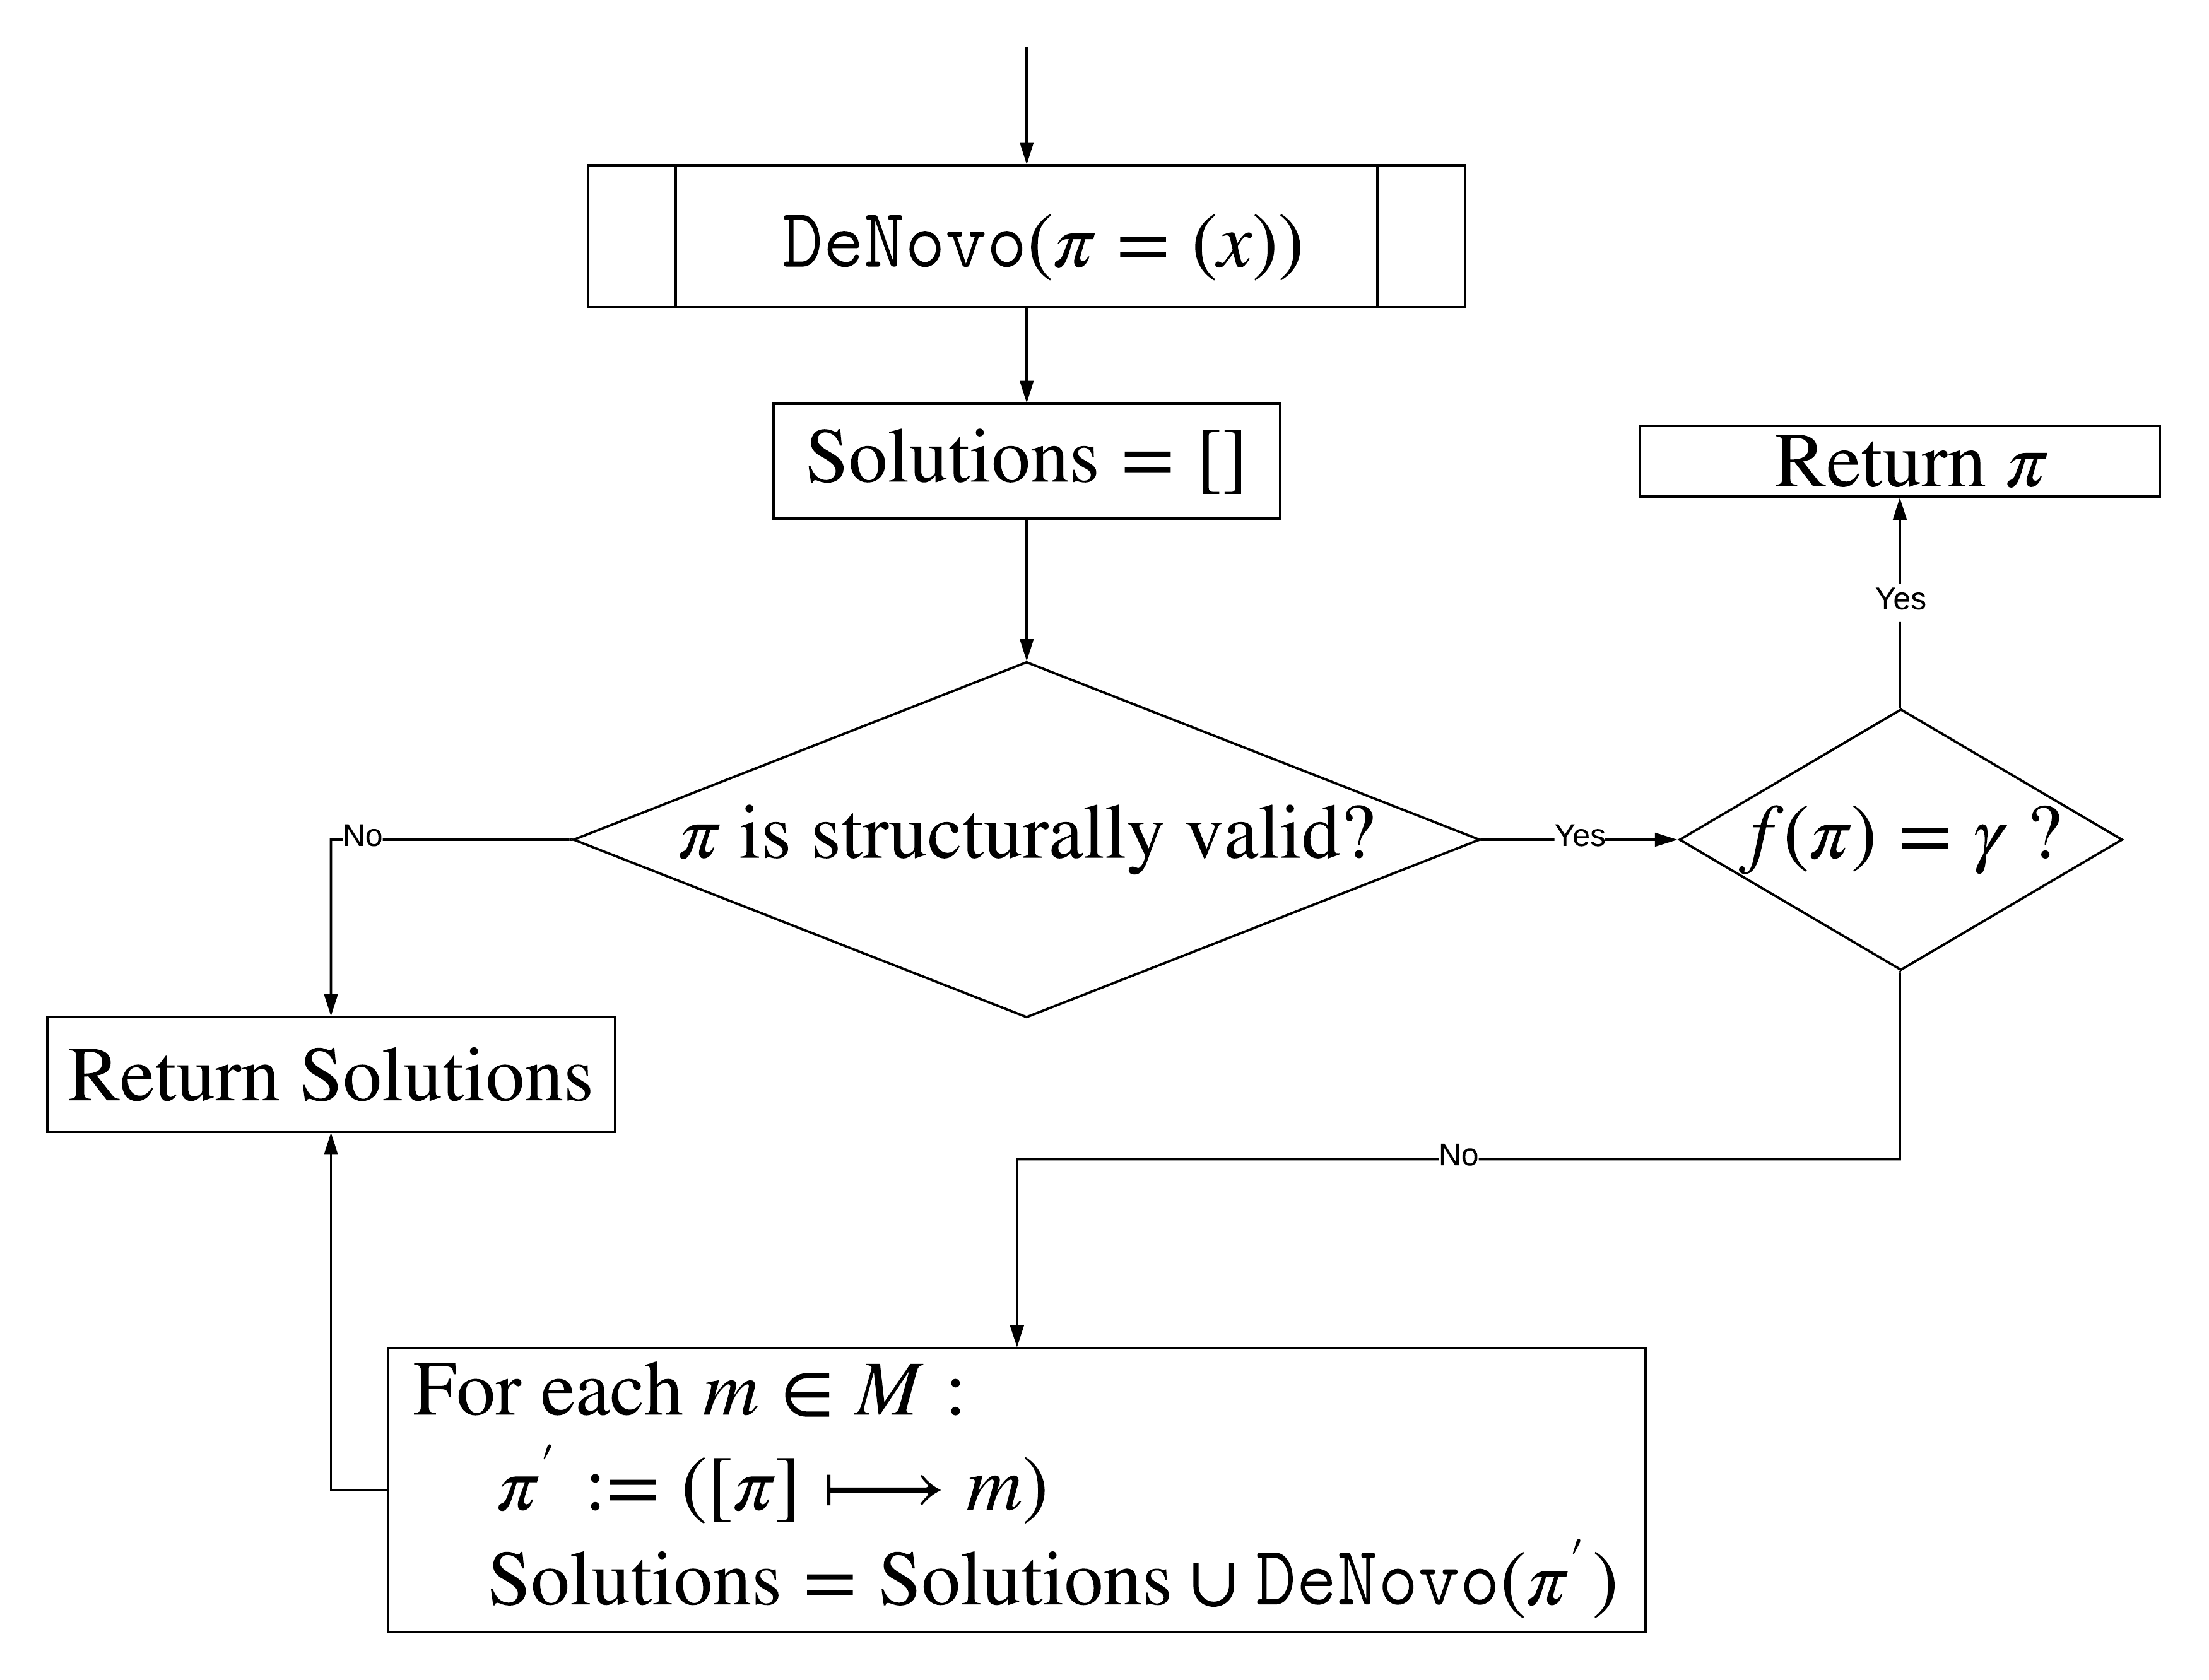
\includegraphics[scale=0.4]{deNovo}
\end{center}
\caption{A breadth-first search algorithm for De Novo SCP search with SCP Task $\Pi=(x,M,\gamma,f())$.}
\label{fig:deNovo}
\end{figure}

\subsection{Insertion Search}\label{ssec:insertion}

Changing the structure of an existing SCP allows researchers to model deviations from standard reasoning for a task. For example, in Section~@TODOref we show that slight modifications to an SCP that models the standard case of the suppression task can lead to an SCP which is able to model reasoners who achieve that classical valid conclusion that she will study late in the library.

The insertion search modifies an existing SCP:
\[\pi=(s_i \longmapsto A_0 \longmapsto ... \longmapsto A_n)\]

to produce a new SCP:

\[
\pi'=\{(s_i \longmapsto B^*_0 \longmapsto A_0 \longmapsto \longmapsto B^*_1... \longmapsto  B^*_n \longmapsto A_n \longmapsto  B^*_{n+1})\}
\] 

Where $B^*_i = (B_0\longmapsto ...\longmapsto B_n)$, $B \in M$  or is the trivial operation $T$ which returns input state point as output. When describing the SCP, $T$ operations are generally omitted.

In general, Insertion Search is a more difficult search type than De-Novo Search (which is equivalent to an Insertion Search in which the initial SCP is empty). The reason for this is that it is possible for a single insertion to result in an invalid SCP, but adding additional cognitive states may revalidate the SCP (Proof~\ref{proof:insertionSearch}).

This consideration means that it is potentially necessary to insert an unbounded number of new cognitive operations at each point in $\pi$ to find those insertions which are valid. When the total number of new cognitive operations to insert is bounded by $N$, however, it becomes possible to generate every possible subsequence of operation insertions of length $\geq N-k$, where $k$ is the number of insertions already used in the search, for each position $B^*_i$ and determine for which of the resulting SCP cognitive operations sequences $f(\pi')$ is valid.

Figure~@TODOfigure illustrates the process of bounded breadth-first search for Insertion Search.

\begin{proof} \label{proof:insertionSearch}
Given a set of cognitive operations $M$, an external activation function $f()$, and an initially valid SCP $f(\pi)$, $\pi=\{s_i \longmapsto A_0 \longmapsto ... \longmapsto A_n\}$, $A_i \in M$, inserting multiple operations into $\pi$ to create cognitive sequence $\pi'$ may result in a valid SCP $f(\pi')$, when inserting only one operation would result in an invalid SCP.

\begin{itemize}
\item Assume hybrid validity (Section~@TODOsection).
\item Let $f(\pi)=\{True if V is defined\}$, $\gamma = True$.
\item Let $A_x$ be a cognitive operation which transforms an input state point of structure $\{KB, V\}$, where $KB$ contains a set of logical formula of the form $head \leftarrow body$ and every rule in $V$ is of the form $variable \leftarrow value$, where $variable$ is an atom and  $value=\top$ into an output state point of structure $\{KB'\}$, $KB'=(KB \cup V)$.
\item Let $A_y$ be cognitive operation which transforms an input state point of structure $KB'$ into an output state point of structure $\{KB, V\}$ where $V$ contains every rule of the form $head \leftarrow body$, where $head$ is an atom and $body=\top$ and $KB= KB' \setminus V$.
\end{itemize}
\item if $f(\pi)$, $pi=(s_i)$ is a valid SCP, then $f(\pi')$, $\pi'=(s_i\longmapsto A_x)$ is an invalid SCP and $f(\pi'')$, $\pi''=(\pi'\longmapsto A_y)$ is valid.
\end{proof}













\chapter{Cognitive Operations: The Cognitive Toolbox} \label{chp:toolbox}
%reference that paper that shows the improvements in machine learning
\section{Overview}
As discussed in Section~\ref{ssec:intu},and illustrated in Figure~@TODOref the simplest imaginable description of sequential human cognition consists of a single step transforming the initial task information (along with background information) into an epistemic state that can be externally interpreted to choose a response. That is, $\mu=(\pi=(S_i \longmapsto m),f())$ can model any cognitive task with a complex enough definition of $m$.

To understand why this is poor choice of SCP, consider a general limitation of the SCP framework: we can only change the output of an SCP by changing the initial epistemic state, or by inserting/deleting a cognitive operation at an existing state point. Consider a case where the initial epistemic state is immutable. Thus, for $f(x \longmapsto A)$, the only possible changes are: $f(x \longmapsto \bar{B} \longmapsto A \longmapsto \bar{B})$, $f(x \longmapsto A \longmapsto \bar{B})$, $f(x \longmapsto \bar{B} \longmapsto A)$, $f(x \longmapsto \bar{B})$, and $f(x)$. Where $\bar{B}$ denotes the action of drawing some sequence of random, but valid cognitive state transitions. There is no way to change the operations that occur in $A$. Thus, even though Figure~@TODOref may be an appropriate model for the general reasoner of a given task, it imposes the explicit assumption that all other test subjects who achieved differing results, achieved only by completely ignoring the black-box process the general reasoners used, or else by inserting new operations only at the very start or end of the processing task. In Section~\ref{sec:supSCP} and Section~\ref{{sec:wstSCP}} we will explore examples of cases where assumptions like that are simply not reflected by empirical data. 

Instead of using a single black-box operation to describe all cognition, it follows logically to use multiple smaller black box operations, each taking a state point as input and resulting in a state point as output. Using this interpretation, cognitive operations for the general reasoner should be as extensive as possible, provided that they do not force implausible changes to describe deviant users or when used in other cognitive tasks. Figure~@TODOref captures this intuition as it applies to the Weak Completion Semantics. Indeed, as a non-monotonic logic that is already explicitly divided into discrete steps in the literature @TODOref, obvious candidate cognitive operations present themselves.

It is worth noting that this increased ability to model deviant reasoners comes at the cost of forcing more state points into the SCP being used.

The remainder of this section is devoted to expressing the exact properties, limitations, and concrete descriptions of cognitive operations, as well as defining several well-founded cognitive operations algorithmically with respect to their preconditions, effects, and output properties in Section~@TODOref.

\section{Cognitive Operation Space}
%then SCP space is cog op space size ^^ scp length
In principle, the number of cognitive operations available for use in an SCP is unlimited. We denote the space of all cognitive operations $\Omega$, and the space of all pCTMs $(A_0 \in \Omega \longmapsto ... \longmapsto A_n \in \Omega)$ with $\Omega^*$. There cannot and never will be an exhaustive search procedure to evaluate every possible way of manipulating an epistemic state (Proofs~\ref{proof:infiniteSCPs} and \ref{proof:infiniteSCPLength} illustrate the existence of valid SCPs for infinitely many different cognitive operations and valid SCPs of any length, respectively). However, there are ways of limiting the number of allowable cognitive operations. Lemma~\ref{lem:uniredundant} defines those cases in which there is redundancy in the set of all possible cognitive operations, Lemma~\ref{lem:taskredundant} focuses this concept on specific cognitive tasks which are to be modelled using SCPs.

The total number of possible non-trivial SCPs of length $L$ for an SCP Task is given by $(|M|^L - R)$ where $|M|$ is the number of elements in the set of cognitive operations $M$, and $R$ is the number of possible non-overlapping task redundant SCPs for the task. @TODOdefineOverlappingRedundantSCPs


\section{A Limited Set of Allowable Operations}
In practice it is impossible compute the set of all candidate SCPs when the set of allowable cognitive operations $M$ in a planning task is $\Omega^*$ or even $\Omega$. Without a length constraint Proof~\ref{proof:infiniteSCPLength} shows that it is not even possible to compute all possible SCPs for many SCP tasks with a finite set of allowable operations. Table~\ref{tbl:solutionSpace} summarises the properties of solution space under different SCP task conditions.

\begin{table}
\begin{center}

\begin{tabular}{ c c c c}
 \textbf{$M$} & \textbf{Finite Length Constraint} & \textbf{Finite Solution Space} & \textbf{Guaranteed Solution}\\ 
 $\Omega^*$ & None & \text{\sffamily X} & \checkmark \\ 
 $\Omega^*$ & Yes & \text{\sffamily X} & \checkmark \\ 
 $\Omega$ & None & \text{\sffamily X} & \checkmark \\ 
 $\Omega$ & Yes & \text{\sffamily X} & \checkmark \\  
 finite &  None & not guaranteed & \text{\sffamily X}\\  
 finite &  Yes &  \checkmark & \text{\sffamily X}
\end{tabular}
\caption{Solution space considerations of SCPs tasks as determined by length constraints and choice of cognitive operations.}
\label{tbl:solutionSpace}

\end{center}
\end{table}

\subsection{A Limited Set of Cognitive Operations}\label{ssec:limCogOp}
Readers should recognize that using the space of all possible cognitive operations for $M$ results in a computationally impossible task. No matter the other conditions imposed there will be infinitely many solutions to the given SCP task which satisfy $f()$.

But, beyond being just computationally infeasible, there are more empirical and philosophical objections to this approach. The first is that the human brain itself does not have infinite processing or space capabilities and so any model which allows for unrestricted data sizes in the set of allowable cognitive operations $M$ or in the number of resultant state points $M$ is not biologically well-founded\footnote{Because $\Omega$ is the set of all possible cogntive operations there must be at least one $m \in M$ such that, for any given input $x$, $x\longmapsto m$ results in a state point of information content greater than the capacity of any storage system to hold.}. 

The second considerations is that there is considerable evidence in the literature that many problems can be modelled using logical frameworks which describe cognitive behaviour across a variety of tasks @TODOref. These frameworks reflect a more generally philosophy in cognitive psychology which is the idea of consistent cognitive motifs in reasoning. Using an infinite $M$ shows no discrimination at the time of task-formulation between those operations for which there is significant evidence and those which are fundamentally improbable.

\subsection{A Limited SCP Length}
As discussed in Section~\ref{ssec:limCogOp}, the human brain is constrained by a set of physical computational and storage limitation. In all case except those which are trivial or repetitive it would be computationally infeasible for the human mind to mimic an infinitely long SCPs. For this reason, SCPs of infinite length, though possible in a mathematical formulation, tend to violate the spirit of the SCP Framework which is to \textit{accurately} model human cognition processes, not simply their conclusions.

It is worth noting that SCPs containing infinite loops can exist and can be evaluated at any time point $n$, they simply cannot be evaluated in their entirety.

\section{Purpose-Selected Cognitive Operations}
\subsection{Overview}

This section discusses the intuition and precise definition of several cognitive operations which will be used throughout the remainder of this paper. These operations allow the SCP Framework to mimic non-monotonic logics for the experiments discussed in Chapter~TODOchapter.

A cognitive operation $m$ is always evaluated in terms of each base point of input state point, and each base point can be considered independent from the others. For these definitions, a base point $\bar{p}$ is assumed as input and a state point is returned as output. Function $\chi(\bar{p})$ determines the validity validity of the input base points. $\Sigma_\chi$ is called the input alphabet and defines the minimal set of an variables names which must be present in $\bar{p}$ for the operation to be allowable.

Accessing a specific element $\alpha_k$ in the structural variables of base point $\bar{p}=(\alpha_1,..,\alpha_n)$ is short-handed to $\bar{p}[\alpha_k]$. $\bar{p}[\alpha_k]$ returns $\alpha_k$ if and only if $\alpha_k \in \bar{p}$ and returns the empty set otherwise. This indexing notation is also used to append a structural variable to $\bar{p}$ and $\bar{p}[\alpha_j]:=t$ removes $\bar{p}[\alpha_j]$ from $\bar{p}$ if it already exists and creates a new structural variable $\alpha_j=t$ in the resulting state point $p'$.

\subsection{Preconditions}

The input alphabet $\Sigma_\chi=\{\alpha_1, ..., \alpha_k\}$ of a cognitive function $m$ describes the set of structural variables which must be present in the epistemic states $\bar{p}$ of the input state point $p$. The alphabet of structural variables in $p$ is given by $\Sigma_p$. Hybrid validity, as defined in Section~\ref{ssec:validity}, can be algorithmically illustrated as follows:

\begin{algorithm}[H] \label{cogOp:th}
\SetAlgoLined
\SetKwProg{Fn}{Function}{ is}{end}
\Fn{$\Sigma_{\chi}$ ($\bar{p}$)}
{
$\Sigma_{\chi}=\{\alpha_1,...,\alpha_n\}$\;
\eIf{$\forall v \in \Sigma_\chi, v \in \Sigma_p$}
{
\Return ``Defined"
}
{
\Return ``Undefined"
}
}

\caption{$\chi$($\bar{p}$): Hybrid validity requirements for $J[p,m]$ to be defined.}
\end{algorithm}

All cognitive operations which we define in this section will be assumed to have a known $Sigma_\chi$ and will only proceed to their effect $e$ if $\Sigma_{\chi}(p)=$ ``Defined''.
The output state point of a defined $J[\bar{p},m]$ is the returned value of $m[e](\bar{p})$.

\subsection{Propositional Logic}
%no requirement of sequence, just exhaustive search
%not computationaly valid, NP-complete is too hard for human brain
An SCP for propositional logic must be able to take a set of rules and facts and draw the set of all valid inferences from that set using the standard propositional rules discussed in Section~@TODOref. To that purpose, we introduce a cognitive operation called \texttt{th} which draws all classically valid inferences from a set of logical rules\footnote{The reason that we do not introduce the functionality of the \texttt{th} cognition operation in the external evaluation function $f()$ is that doing so would make it impossible to directly use the derived theorems as part of another SCP.}.

\texttt{th} is by its nature a contrived cognitive operation and there is no expectation that it truly reflects human cognition. Instead, it serves as a benchmark operation with which to compare the results derived from knowledge base-driven logical approaches. Even a simpler congitive operation called \texttt{SAT} which determines if the given knowledge base it satisfiable still represents an \textit{NP-complete} (@TODOref) problem and is infeasible for any large knowledge base.

However, variations on the intuition of these two problems have real applications in cognitive modelling with SCPs and will be discussed throughout this section.

\begin{algorithm}[H] \label{cogOp:th}
\SetAlgoLined
\SetKwProg{Fn}{Function}{ is}{end}
\Fn{$e$($\bar{p}$)}
{
$\bar{p}[S]:=\bar{p}[S] \cup [(\text{atom name} \leftarrow \text{value}) |$ ($\text{atom name},\text{value}) \in \bar{p}[V]$ and $\text{value} \neq u$\;
$\bar{p}[S]:=\bar{p}[S] \cup [A$ | clause $A$ would not make $\bar{p}[S]$ inconsistent$]$\;
$\bar{p}[V]:=[B$ | $B \leftarrow body \in \bar{p}[S]$ and $ I(body)=\top$ or $I(body)=\bot$]\; 
\Return $\bar{p}$
}

\caption{\texttt{th}$(\bar{p})$: generates the potentially infinite set of possible classical inferences from $\bar{p}[S]$.}
\end{algorithm}

A realised SCP $r=(k=K[\pi],f())$ is said to \textit{model the classical inference}, if $f(k) = f(s_i \in \pi \longmapsto \texttt{th})$. An SCP $\pi$ is said to model the classical inference if some realised SCP generated from $\pi$ models the classical inference.


\subsection{Variable Insertion}

Variable insertion is a single cognitive operation with a highly intuitive interpretation and justification. By its nature, the set of variables $V \in \bar{p}$ in an epistemic state $\bar{p}$ is not a true possible world (as discussed in Section~\ref{ssec:epiprops}), and may omit variables present in the real possible world. But one these variables may become apparent later. For example, when interpreting a conditional as a license for implication, or when storing the result of a calculated mathematical problem.

It seems reasonable then that a cognitive operation \texttt{addV} which appends a variable to base point $V$ would be required to expand to the knowledge base to incorporate new facts.

\begin{algorithm}[H] \label{cogOp:addV}
\SetAlgoLined
\tcc{The variable to be added, defined before SCP execution.}
$v:= \alpha=(\text{atom name},\text{value})$\;
\SetKwProg{Fn}{Function}{ is}{end}
\Fn{$e$($\bar{p}$)}
{
\tcc{Remove all possible assignments of the variable from the list of variables}
$\bar{p}[V]:=\bar{p}[V] - [\text{atom name}, x \in \text{Domain}_\text{atom name}] $
\tcc{Add the new variable and its assignment to the list of variables}
$\bar{p}[V]:=\bar{p}[V] \cup \alpha$\;
\Return $\bar{p}$
}

\caption{\texttt{addV}$(\bar{p})$: adds a variable $v$, defined \textit{a priori}}
\end{algorithm}

In order to ensure that the SCP still acts as a pipeline of information, it is necessary that $\texttt{Add}\alpha$ for variable $\alpha=(\text{atom name, value})$ is defined as part of the allowable operations of the SCP Task $\Pi$ which generates the SCPs and realised SCPs that will make use of it. The core principle of this pipeline framework is that each usable component (cognitive operation) of that framework which is not the input value should not be modified.

\subsection{Variable Deletion} \label{ssec:deletion}
Following on the from the $\texttt{addV}$ operation, the $\texttt{removeV}$ operations captures human intuition of forgetting. Consider the sequence of numbers: 1, 44, 27, 8, 0 , -4, 6, 7, 346, 7, 74, 7, 234, -55, 2.4, 18. Now without looking back at the numbers, ask yourself some questions: how many numbers were there? Were any of them prime? How many numbers were repeated? In all probability you are not entirely sure. This simple thought experiment provides support for our first extension, the idea that variables can be ``forgotten", that is, that information that existed in the knowledge base at one point in time might no longer exist at a later timepoint. 

This is not the only imaginable case where a variable might be removed from the knowledge base of the person being modelled. The size of the knowledge base used for cognitive modelling is always implicitly restricted to relevant variables. Only those variables whose values might reasonably be expected to affect the final conclusions drawn with regard to the research question should be considered. Finding which variables and rules are relevant is, however, non-trivial. For another real-life example, imagine a mystery novel: Three hundred pages of plot descriptions, character actions, and dialogues. In a good murder mystery novel every piece of information that reveals the killer's identity is hidden in the story itself, yet we do not hold every fact and interaction in the book in our epistemic model of the book, so discerning the identity of the killer remains a mystery until the last page. But when the mystery is solved, many details that we internalised while reading (and recall in retrospect) suddenly make the conclusion seem obvious. We have not forgotten this information, we had merely incorrectly deemed it irrelevant at the time and ignored it in our cognitive processing.

Forgetting a variable in an SCP is not-trivial task, just as removing a variable in an AI planning task @TODOref is non-trivial. Multiple intuitions for how it may best be done occur, but we will keep this definition as simple as possible for the examples that will be discussed in Chapter~@TODOref. We introduce three cognitive operations $\texttt{remove}_\top V$, $\texttt{remove}_\bot V$, and $\texttt{remove}_u V$. $\texttt{remove}_\top$ assumes that conditionals and rules which depend on the removed variable are validated by its removal. $\texttt{remove}_\bot V$ assumes that rules and conditionals are invalidated by the removal. $\texttt{remove}_u V$ assumes that no conclusion can be drawn without this information.  These three approaches can be differentiated by these examples:

\begin{itemize}
\item ``If aliens invade, then I will hide in my bunker."
\item ``If I do not fail my exam, then I will graduate.''
\item ``Unless I am a boy, I am a girl.''
\end{itemize}

In the first example, the presumed default position is that I will not hide in my bunker. In the second, the default position is that I will graduate. And in the third example there is no apparent default position. In the absence of the conditions in each each of these conditionals we would probably conclude that, I am probably not hiding in my bunker, I probably graduated, and that my gender is uncertain. This observation implies that a mechanism by which to determine the plausibility of default positions is needed to translate such default theories into a non-monotonic framework. In the absence of such a mechanism we will generally assume $\texttt{remove}_\bot V$, as with the closed-world assumption.

\begin{algorithm}[H] \label{cogOp:removeuV}
\SetAlgoLined
\tcc{The variable to be deleted, defined before SCP execution.}
$v:= \text{atom name}$\;
\SetKwProg{Fn}{Function}{ is}{end}
\Fn{$e$($\bar{p}$)}
{
\tcc{Remove $\alpha$ from the possible world variables.}
$\forall_{\alpha = (\text{v},\text{value}\in \text{domain}(v))} \bar{p}[V]:=\bar{p}[V] - \alpha$\;
\For{$\text{rule}=(\text{head} \leftarrow \text{body}) \in \bar{p}[S]$}
{
\If{$\text{head}=v$}
{
$\bar{p}[S]:=\bar{p}[S]-\text{rule}$\;
}
\If{$\text{v} \in \text{body}$}
{
replace all subclauses $(v \lor \phi)$, $(v \land \phi)\in \bar{p}[S]$ with $(\phi)$\;
}
}
\For{$\text{rule}=(\text{head}|\text{body}) \in \bar{p}[\Delta]$}
{
\If{$\text{head}=v$}
{
$\bar{p}[\Delta]:=\bar{p}[\Delta] - \text{rule}$\;
}
\If{$\text{v} \in \text{body}$}
{
replace all subclauses $(v \lor \phi)$, $(v \land \phi)\in \bar{p}[\Delta]$ with $(\phi)$\;
}
}
\tcc{This is where $\texttt{remove}_\bot V$ differs from $\texttt{remove}_\top V$, and  $\texttt{remove}_u V$ }
replace all rules $\text{head} \leftarrow v \in \bar{p}[S]$ with $\bot$\;
replace all rules $\text{head} \leftarrow \lnot v \in \bar{p}[S]$ with $\lnot \bot$\;
replace all rules $(\text{head}|v)$ with $\bot$\;
replace all rules $(\text{head}|\lnot v)$ with $\lnot \bot$\;

\Return $\bar{p}$
}

\caption{\texttt{remove}$_\bot$V$(\bar{p})$: removes a variable name $v$, defined \textit{a priori}}
\end{algorithm}

\subsection{Variable Silencing}
\subsection{Variable Fixation} \label{ssec:variableFixing}
The next case of a potential complex operation to add to the search space of our SCPs is the idea of Variable Fixing. The idea that some  conclusions can be fixed \textit{a priori}. This operation may prove contentious to those who are experienced with mathematical logic, but holds some merit when justified from a psychological perspective. 

Consider a person who strongly doubts the effectiveness of vaccines, we will call her Karen. Karen started her day convinced that giving her child the MMR vaccine is more dangerous than the disease itself. Later that day Karen spoke to her doctor who strongly advised that she vaccinate her child. He offered her a variety of peer-reviewed papers and studies that showed the relative safety of the vaccination. Karen listened carefully to the trained medical professional, and then went home. After some thought Karen decided that he was wrong, and her opinion on vaccines didn't change.

In this example Karen shows a very powerful type of cognitive bias, the unwillingness to change her opinions, despite powerful evidence to the contrary. This phenomenon has been observed across a great many fields of study, from medical psychology \citep{brown2010omission} \citep{wroe2005feeling} to political sciences\citep{tappin2017heart}. In the context of cognitive modelling with logics, it indicates that some mental rules or variables are immutable, regardless of new evidence or valid beliefs that would logically contradict them. Non-monotonic logics, as a class, are already capable of dealing with bias effects, as non-monotonic logics are built on the basis of a preference operation.

In order to implement this operation, we will make use of the categorization variable $R$ first discussed in Section~@TODOref.

\begin{algorithm}[H] \label{cogOp:addV}
\SetAlgoLined
\tcc{The variable to be fixed, defined before SCP execution.}
$v:= (\alpha = (\text{atom name}, \text{value}))$\;
\SetKwProg{Fn}{Function}{ is}{end}

\Fn{$e$($\bar{p}$)}
{
$\bar{p}[V]:=\bar{p}[V] - (\text{atom name}, \text{value} \in \text{domain}) \in \bar{p}[V]) \cup \alpha$\;
$\bar{p}[R][\text{fixed}]:= \bar{p}[R][\text{fixed}] \cup v$\;
\Return $\bar{p}$
}

\caption{\texttt{FixV}$(\bar{p})$: fixes a variable name $v$, defined \textit{a priori}}
\end{algorithm}


This algorithm removes `$\text{atom name}$' from the possible world $V$ and readds it with the value to which it is to be fixed. The atom is then added to the list of fixed variables kept by $\bar{p}[R]$. This list of fixed variables is used by other operations which evaluate state points later in the SCP or realised SCP, and, as per their encoding, they will not modify the assignment of this variable.

\subsection{Adding Abnormalities}

As discussed in Section~\ref{ssec:condInterpretation}, one way to interpret conditionals in reasoning tasks is as licenses for implication. One possible definition for a cognitive operation that performs this same task by transforming defeasible conditional facts to propositional logic rules is as given by Algorithm~\ref{cogOp:addAB}.

@TODOdefiniesigmachiasalphabetofvariablesincogop

\begin{algorithm}[H] \label{cogOp:addAB}
\SetAlgoLined
\SetKwProg{Fn}{Function}{ is}{end}
\Fn{$e$($\bar{p}$)}
{
\tcc{Variables for which an abnormality has already been created}
\For{$(\psi|\phi) \in \bar{p}[\Delta]$}
{
$k:=$ the lowest natural number for which $\text{ab}_k \notin \bar{p}[S]$\;
$\text{all dependencies}:= [A | (\psi|A) \in \bar{p}[\Delta]]$\;

\For{$A \in \text{all dependencies}$}
{
$\text{head}:=\psi$\;
\tcc{All other variables which can make $\psi$ true are treated as though they could also falsify $\psi$.}
$\text{current dependencies}:= \text{all dependencies} - \text{A}$\;
\If{$\text{current dependencies} = \{\}$}
{
$\text{current dependencies}:=\bot$\;
}
$\text{body}:=(\text{current dependencies}_1 \lor ... \lor \text{current dependencies}_n)$\;

\tcc{Add the conditional as a license for implication to the set of rules.}
$\bar{p}[S]:= \bar{p}[S] \cup (\text{head} \leftarrow A \land \lnot \text{ab}_k)$\;
$\bar{p}[S]:= \text{ab}_k \leftarrow \lnot body$\;

}
\tcc{Add the new abnormality to the possible world $V$.}
$\bar{p}[V]:= \bar{p}[V] \cup (\text{ab}_k,u)$\;
}
\tcc{Remove all conditionals now that they have been interpreted as licences for implication.}
$\Delta:=\{\}$\;
\Return $\bar{p}$
}
\caption{\texttt{addAB}$(\bar{p})$}
\end{algorithm}

\subsection{Weakly Completing}


Weak completion is an essential part of the WCS. Under the assumption that the WCS is a valid representation of human cognition in at least one scenario, any comprehensive set of cognitive operations $M$ must be able to mimic the Weak Completion of a knowledge base. Algorithm~\ref{cogOp:wc} shows one way in which this can be achieved.

\begin{algorithm}[H] \label{cogOp:wcs}
\SetAlgoLined
\SetKwProg{Fn}{Function}{ is}{end}
\Fn{$e$($\bar{p}$)}
{
Replace all rules $\in \bar{p}[S]$ of the form $A\leftarrow \text{body}_1,...,A\leftarrow \text{body}_n$ with $A\leftarrow \text{body}_1 \lor ... \lor \text{body}_n$ \;
Replace all occurrences of $\leftarrow \in \bar{p}[S]$ with $\leftrightarrow$ \;
\Return $\bar{p}$
}

\caption{\texttt{wcs}$(\bar{p})$}
\end{algorithm}



\subsection{Semantic Operator}

Another essential step in the WCS, the semantic operator is used to assign all variables to either True or False (explictly), or to Unknown (implicitly). Algorithm~\ref{cogOp:semantic} illustrates one way in which this cognitive operation can be implemented for any epistemic state of the form $s=(KB,V,...)$.

\begin{algorithm}[H] \label{cogOp:semantic}
\SetAlgoLined
\SetKwProg{Fn}{Function}{ is}{end}
\Fn{$e$($\bar{p}$)}
{
\tcc{All least models that can achieved by applying the semantic operator to the current state point.}
$p'= \{phi_{SvL}(\bar{p})\}$\;
\Return $p'$
}

\Fn{$\phi_{SvL}$($\bar{p}$}
{
\If{there exists a clause $A\leftarrow \text{body} \in \bar{p}[S]$ with $I_V(body)=\top$ }
{
\If { $\text{A} \not\in \bar{p}[\text{fixed}]$}
{
$\bar{p}[V][A]:=\top$
}
}
\If{there exists a clause $A\leftarrow \text{body} \in \bar{p}[S]$ and for all clauses $A\leftarrow \text{body} \in \bar{p}[S]$ we find $I_V(body)=\bot$}
{
\If { $\text{A} \not\in \bar{p}[\text{fixed}]$}
{
$\bar{p}[V][A]:=\bot$
}
}
\Return $\bar{p}$
}

\caption{\texttt{semantic}$(\bar{p})$}
\end{algorithm}

\subsection{Adding Abducibles} \label{ssec:abd}
Next, we define a cognitive operation which uses the set of possible abducibles, given by $\bar{p}['R']['abducibles']$. We have already used the intuition of this operation to handle the WST and derive the general answer set. Later we will see that it can also be used to model individual reasoners in the Suppression Task. \texttt{AddExp} adds possible explanations $\eta$ to the set of rules $S$ in the epistemic state and is defined as follows:

\begin{algorithm}[H] \label{cogOp:addExp}
\SetAlgoLined
\SetKwProg{Fn}{Function}{ is}{end}
\Fn{$e(\bar{p})$}
{
abducibles:=$\bar{p}[\text{`abducibles'}]$\;
$p':=[]$\;
\For{every unique subset $A \in$ abducibles }
{
newP := $\bar{p}$\;
$\text{newP}['S']=\text{newP}[\text{`S'}] \cup \{a \in A\leftarrow \top\}$\;
$\text{newP}['\eta']=A$\;
$p':=p' \cup \text{newP}$\;
}
\Return $p'$
}

\caption{$\texttt{addExp}$}
\end{algorithm}


\subsection{Default Inferencing}
If we assume that Reiter's default logic is a valid model of cognition for at least one task, it follows that an comprehensive formulation of $M$ must encode a cognitive operation for drawing inferences from a set of default rules. Figure~@TODOref illustrates the procedure for drawing such inferences from an epistemic state state of the form $s=(KB,V,D)$ where $KB$ is a set of inference rules, $V$ is mapping of variable names onto variable values, and $D$ is a set of default rules of the form $\frac{condition:exception}{conclusion}$ @TODOrewriteEquationWithStandardSymbols.



\section{Cognitive Operations as Aggregates}
%talk about combining existing cognitive operations for which there is strong evidence
An obvious and interesting idea follows from Proof~\ref{proof:aggregateValid} which is the idea of finding well-founded, uninterrupted epistemic operation sequences which are effective in modelling a variety of tasks and representing them as a single epistemic operation. We call this approach \textit{aggregating}, and it draws inspiration from recent advances in the field of reinforcement learning @TODORef in which simple tasks previously achieved are used as allowable actions when attempting to solve complex tasks.

This approach introduces the desirable property of shortening the total length of the SCP for a given set of cognitive tasks. However, it is evident from Proof~\ref{proof:aggregateExpressiveness} that any SCP task in which an aggregated subsequence of operations replaces those individual operations in $M$ may be less expressive than the same formulation in which the aggregated operations are still present.

For example, the cognitive processes \texttt{wc} and \text{semantic} could be combined together to form a single \text{wcs} operator as follows:



The use of aggregates then, is a trade-off between sacrificing cross-reasoner accuracy and optimising a set of desirable heuristic properties such as length minimisation.

In many ways this compromise follows the philosophy of cognitive modelling in general. A neuron-by-neuron approach to predicting human behaviour (if one were ever possible) would give us extreme accuracy in modelling any human reasoner, but is too complex to be practical, and even if it were, would provide no abstracted information with which to find common motifs and inferences among reasoners. On the other extreme, modelling reasoners as (\textit{input}, \textit{output}) pairs perfectly captures the average predictions of a population, but proves very inaccurate for unseen individuals. State-of-the-art approaches to cognitive modelling like neural networks and non-monotonic logical frameworks seek generalizations which accurately capture the responses of most reasoners across as many tasks as possible by approximating human motifs in human reasoning and applying across multiple tasks and inputs.

A researcher could decide that it is unreasonable to expect any cognitive operations to seperate \texttt{wc} and \texttt{semantic}, as the both form part of the same nonmonotonic logic. They might then create the new aggregate complex operation \texttt{wcs} which applies the WCS in its entirety as follows:

\begin{algorithm}[H] \label{cogOp:wcs}
\SetAlgoLined
\SetKwProg{Fn}{Function}{ is}{end}
\Fn{$e$($\bar{p}$)}
{
$\bar{p}':=\texttt{wc}(\bar{p})$\;
$p':=\texttt{semantic}(\bar{p'})$\;
\Return $p'$
}

\caption{\texttt{wcs}$(\bar{p})$}
\end{algorithm}

They could even go a step further and define the cognitive operation $\texttt{abwcs}$ which first interprets the conditionals in $p[\Delta]$ and then applies the WCS to the result. This algorithm is as follows:

\begin{algorithm}[H] \label{cogOp:abwcs}
\SetAlgoLined
\SetKwProg{Fn}{Function}{ is}{end}
\Fn{$e$($\bar{p}$)}
{
$\bar{p}':=\texttt{addAB}(\bar{p})$\;
$\bar{p}':=\texttt{wc}(\bar{p})$\;
$p':=\texttt{semantic}(\bar{p'})$\;
\Return $p'$
}

\caption{\texttt{abwcs}$(\bar{p})$}
\end{algorithm}

The reader will note that $\texttt{abwcs}$ now provides precisely the same functionality as the examples of the WCS we examined in Chapter~\ref{chp:experiments}, and Chapter~\ref{chp:model} will show that these three operations in sequence can indeed be modelled in the SCP framework and come to the same conclusions as when the WCS is applied in the original experiments.

The question of how to generate appropriate complex operation aggregates is a complex problem and is not discussed further in this thesis. It is, however a topic in which the author has significant interest.


\section{Epistemic State Structure Changes with Cognitive Operations}
%e.g. going to WCS to Default
The conception and mathematics of cognitive operations which produce output epistemic states points which differ in structure from the epistemic input structure are fairly straightforward.

Some cognitive operation $A$ with input base point structure $\textrm{struct}(s_k)$ and output base point structure $\textrm{struct}(s_{k+1})$ is called a \textit{structural transformation operation} if and only if $\textrm{struct}(s_k) \ne \textrm{struct}(s_{k+1})$.

The intuition behind structural state changes goes back to Albert Einstein's quote that opened this thesis ``Everything should be made as simple as possible, but no simpler.". In theory there is no restriction on SCP structure that would prevent every epistemic state passing an arbitrarily large number of variables and arguments. An SCP meant to represent a cognitive task where participant responses are consistent with propositional logic, for exmaple, could be accurately represented with an initial state $s_x=(S)$ where $S$ is simply the knowledge base of facts and rules given; but a researcher might equally use an epistemic state $s_y=(S,V)$ where a variable $V$ is intended to store the values of each variable in $S$; or even $s_z=(S,V,D)$ where $D$ is a set of default rules. All three of these approaches would give an SCP the information required to evaluate the propositional task, but, if we know the task structure does not deal with uncertainty or show variation in reasoner responses, it becomes apparent that the set of default rules $D$ is unnecessary.

All of the possibilities given hold for the propositional task because $s_y$ and $s_z$ are both supersets of $s_x$ and $s_x$ is sufficient to model the task. Thus, provided the researchers do not believe that the task will make use of cognitive operations which require more complex state structures, $s_x$ is the simplest solution which meets the requirements of the researchers.

An obvious extension to the discussion above is the fact that a transformation from one state point structure to another when the input structure is a subset of the output structure is as easy as appending more structural variables to the input state. This transition hold in the example above in which a propositional logic compliant state point $s_x$ could be transformed into a WCS compliant state point $s_y$ or a default rule compliant state point $s_z$.

Unfortunately, structural change by appending variables are not universal obvious cases of structural transformation where they do not apply spring to mind. Such as the case where a more expressive state point must be changed to a less expressive state point structure. Imagine a case where a cognitive operation $B$ transforms a case point of $\textrm{struct}(s_z)$ to one of $\textrm{struct}(s_y)$. An intuitive example of this might be a hypothetical mental operation which handles biases in thinking. A student might begin at an epistemic state which believes ``usually, if I study for tests, I fail" and, through bias confirmation, come to believe ``If i study for tests, I fail", transitioning from a default rule, to immutable rule. 

In cases like this, it is up to the researcher to make several decisions: do I believe that the now empty set of variables $D$ no longer provides meaningful information? And how do I represent the change in the variables still present in the output state? These questions are very often task or function specific and cannot be answered in a general sense.

\section{Two Approaches to Creating Cognitive Operations}
\section{Theoretical Approximation}
%must have empirical basis, but focused on reproducing mechanisms that have been proposed and substantiated in literature
%hand-curated
It seems reasonable that, given our desire to accurately model reasoning in participants, researchers creating cognitive functions for SCPs would choose to limit the set of allowable cognitive operations to those for which there is a sound theoretical basis. The reasons for this choice were discussed in Section~@TODOref.

The first approach to creating cognitive operations we will consider is the use of cognitive operations for which there is already evidence in our existing models of human cognition. This evidence can take a wide variety of forms: it may follow from our knowledge of physics (for example, the impossibility of storing a set of unrelated variables above a certain physical threshold); evolutionary biology (there cannot exist a class of organisms without some kind of reproductive drive); anatomy (there must exist cognitive processes that facilitate voluntary muscle activation); sociology (some neuronal connections seem to restrict the number of close friends a human can maintain @TODOref); or any other field of science. Using this information can allow researchers to predict what cognitive functions may play a role in observed empirical data. 

For the most part, theoretical approximation is a very powerful and well-justified mechanism for determining which cognitive operation could plausibly considered in the cognitive toolbox for a given task. Restricting the space of other cognitive operations which may play a part is also enabled by all the scientific fields mentioned above, complexity theory tells us that humans are unlikely to apply exhaustive classical logic reasoning to a task when the set of variables and rules to be considered is large because of physical limitations related to solving \textit{NP-complete} or harder tasks efficiently.

At present, the foundation of non-monotonic reasoning in cognitive modelling is this theoretical mindset, a well-founded explanation is found by borrowing from a relevent field (often psychology) and then tested against empirical evidence and across multiple cognitive tasks to show evidence that is a reasonable approximation of a mechanism in human cognition.


\section{Empirical Appoximation}
%finding cognitive operations using machine learning
%done by using search techniques to create and explore comparison space
Contrasting theoretical approximation is the field of constrained empirical approximation. Techniques ranging from neural networks and Markov models genetical inspired techniques consistently outperform humans in a huge variety of fields. Drawing on enormous databases of empirical data, modern artificial intelligence researchers have come to view machine learning as the most plausible way to create the first real thinking machine @TODOref.

@TODOfinish

\chapter{Mimicking Non-Monotonic Logics With SCPs} \label{chp:mimick}

\section{The Suppression Task}

\section{The Weak Completion Semantics}



\chapter{Modelling Experiments with SCPs} \label{chp:model}
\section{Overview}
As with any cognitive framework, the most important metric for judging the success of SCPs comes from testing how well SCPs can approximate empirical data across tasks. This chapter will show the suitability of SCPs with a common set of allowable cognitive operations for modelling several well-studied experiments in cognitive modelling.

In particular, we will show that the Wason Selection Task, Suppression Task and @TODO can be modelled at both the general and individual reasoner level with SCPs in a formulation that intuitive and consistent with the WCS approach already described in Section~@TODOref.
\section{Suppression Task}

\begin{figure*}
\begin{center}
 \centering 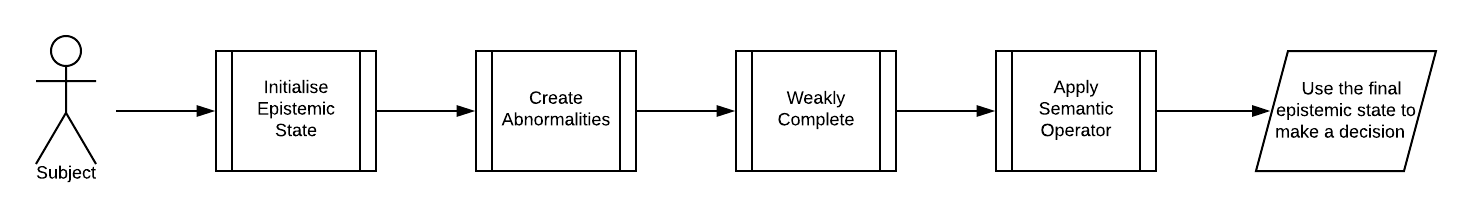
\includegraphics[width=\linewidth]{suppressionSCP_overview}
\caption{A generalised illustration of the WCS in an SCP. }
\label {fig:supoverview}
\end{center}
\end{figure*}

\begin{figure*}
\begin{center}
 \centering 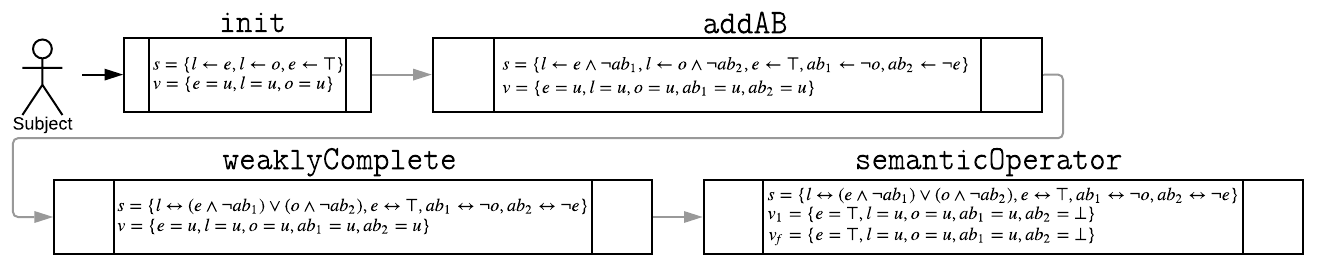
\includegraphics[width=\linewidth]{suppressionSCP_normal}
\caption{The standard case of the Suppression Task, demonstrating the suppression effect. Where the epistemic state in the boxes represents the output of that cognitive operation. $V_f$ represents the assignment of $V$ in the epistemic state in the resulting least model. $V_{i\in \mathbb{N}}$ represents the assignments in $V$ after $i$ iterations of the semantic operator.}
\label {fig:supnormal}
\end{center}
\end{figure*}

Figure~\ref{fig:supoverview} illustrates a generalised SCP to describe the Suppression Task as a series of sequential steps directly mirroring the discrete steps outlined in Section~\ref{sec:sup}, each cognitive operation passing information to the next process\footnote{It is important to note that a diagram like this is valid for \textit{any} cognitive modelling task because any process may be arbitrarily complex and non-sequential. and so the overall linear process of (actor, complex decision, observed results) is always valid for retroactive modelling, and at least as powerful as the non-monotonic logic framework it uses for modelling.}. To model the SCP the implicit sequence of operations in the Suppression Task is systematized and refined into a set of complex operations. Further we introduce an initial epistemic state $s_i=(KB,V,R)$. One interpretation of the requirements of the suppression task $\pi=(s_i,\gamma,M)$ using SCPs and the WCS is as follows: 
 
 
 
 


\[s_i=\{KB_i, V_i, R_i\} \]
\[KB_i=\{e \rightarrow l, \top \rightarrow e, o \rightarrow l\} \]
\[V_i=\{e:u, l:u, o:u\} \]
\[R_i=\{\} \]
\[
\begin{split}
M= \{\texttt{init}, \texttt{addAB}, \texttt{WeaklyComplete}, \texttt{semanticOperator}\}
\end{split}
\]
\[\gamma = (l\models \top) \textrm{ or } (l \models \bot)\]

%@TODO change semanticOper to semanticOperator without line overflowing 

where all cognitive operations require as input and produce as output a state point $p$ where every ground point $\bar{p} \in_s p$ is of format $\bar{p}=(KB,V,R)$; \texttt{init} is always the first cognitive operation and adds the initial variables and rules to epistemic state; \texttt{addAB} adds abnormalities to the current epistemic state using the procedure described in Algorithm~\ref{alg:addAbnormalities} (but now also adds those abnormalities to the variable list of the epistemic state); \texttt{WeaklyComplete} weakly completes the knowledge base of the current epistemic state; and \texttt{semanticOperator} returns an epistemic state that leaves the knowledge base unchanged but updates the variables of that state to return the least model of the epistemic state. \texttt{semanticOperator} follows the same logic seen in Section~\ref{ssec:wcs}, but directly updating $V$ after each iteration of the semantic operator, instead of the externalised variable set $J$. Thus, we ensure that the output state point is able to communicate the result of applying the semantic operator without any structural changes to the epistemic states it contains. As an additional feature of the \texttt{semanticOperator} cognitive operation, if there exists a labelled set in $R$ called $fixed$, then the semantic operator will not set the value of any $v \in fixed$ in the variables list $V$. The goal $\gamma$ states that $l$ should no longer be mapped to unknown in the final epistemic state.



Treating Figure~\ref{fig:supoverview} as an SCP, we observe the sequence of output states seen in Figure~\ref{fig:supnormal}. Note that in the final state $l$ remains mapped to $u$, meaning that the suppression effect is demonstrated.

\subsection{Extending the Suppression Task with SCPs}
The previous example merely showed that SCPs are suitable for modelling the suppression task. In this example we consider one of the most powerful characteristics of SCPs, the ability to model unusual results as deviations from general reasoning. In the original Suppression Task Experiment examined in Section~\ref{sec:sup}, a significant portion of people still believed that she would study late in the library, even though the majority suppressed the inference. Several possible explanations are intuitive, the first and simplest, is the assumption that the reasoner is using classical logic and drawing the classical conclusion. However, what if that is not the case? What if they do reason in exactly the same way as the other reasoners, except for one or two small deviations?

In order to model these non-general reasoners, we consider two possible deviations that could explain the classical result of the Suppression Task: \textit{variable deletion}, and\textit{ variable fixation}. Both of these operations will be discussed in a way that may seem overly prosaic, but it is done to reinforce that we might, reasonably, expect these cognitive operations to occur in day-to-day human cognition.

\subsection*{Variable Deletion} \label{ssec:variableDeletion}
Consider the sequence of numbers: 1, 44, 27, 8, 0 , -4, 6, 7, 346, 7, 74, 7, 234, -55, 2.4, 18. Now without looking back at the numbers, ask yourself some questions: how many numbers were there? Were any of them prime? How many numbers were repeated? In all probability you are not entirely sure. This simple thought experiment provides support for our first extension, the idea that variables can be ``forgotten", that is, that information that existed in the knowledge base at one point in time might no longer exist at a later timepoint. 

This is not the only imaginable case where a variable might be removed from the knowledge base of the person being modelled. The size of the knowledge base used for cognitive modelling is always implicitly restricted to relevant variables. Only those variables whose values might reasonably be expected to affect the final conclusions drawn with regard to the research question should be considered. Finding which variables and rules are relevant is, however, non-trivial. For another real-life example, imagine a mystery novel: Three hundred pages of plot descriptions, character actions, and dialogues. In a good murder mystery novel every piece of information that reveals the killer's identity is hidden in the story itself, yet we do not hold every fact and interaction in the book in our epistemic model of the book, so discerning the identity of the killer remains a mystery until the last page. But when the mystery is solved, many details that we internalised while reading (and recall in retrospect) suddenly make the conclusion seem obvious. We have not forgotten this information, we had merely incorrectly deemed it irrelevant at the time and ignored it in our cognitive processing.

The exact details of how to delete a variable from a knowledge base are non-trivial, and there is no best practice for doing so. But in simple cases the process can be intuitive. Let \texttt{delete} be a complex operation. \texttt{delete} takes as input any state point and is applicable for any ground point $\bar{p}$ with variable list $V \in \bar{p}$ and categorization variable $R$ with ($delete:V_{del}) \in R$, where $V_{del}$ is the set of variable names to delete. For every $v \in V_{del}$ remove all rules from $KB$ that have $v$ as body or head of the clause, and remove $v$ from $V$. Then remove $delete$ from $R$.

In the case of the Suppression Task we argue that one cognitively valid reason for drawing the classical conclusion to the task may be forgetting (or disregarding) the variable $o$. Figure~\ref{fig:supmod} illustrates this case, and shows how the insertion of a complex operation can completely change the final epistemic state.

\begin{figure*}
\begin{center}
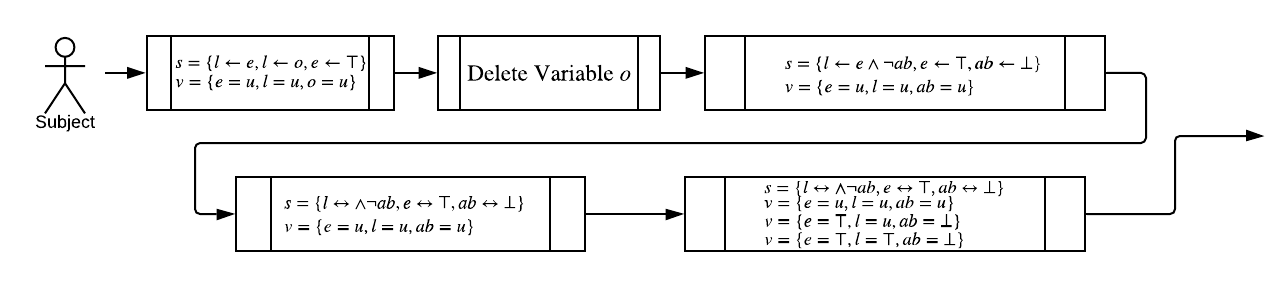
\includegraphics[width=0.85\linewidth]{suppressionSCP_mod}
\end{center}

\caption{The Suppression Task in which the additional operation of deleting the variable $o$ occurs.}
\label{fig:supmod}
\end{figure*}

\subsection*{Variable Fixing} \label{ssec:variableFixing}

\begin{figure*}
\begin{center}
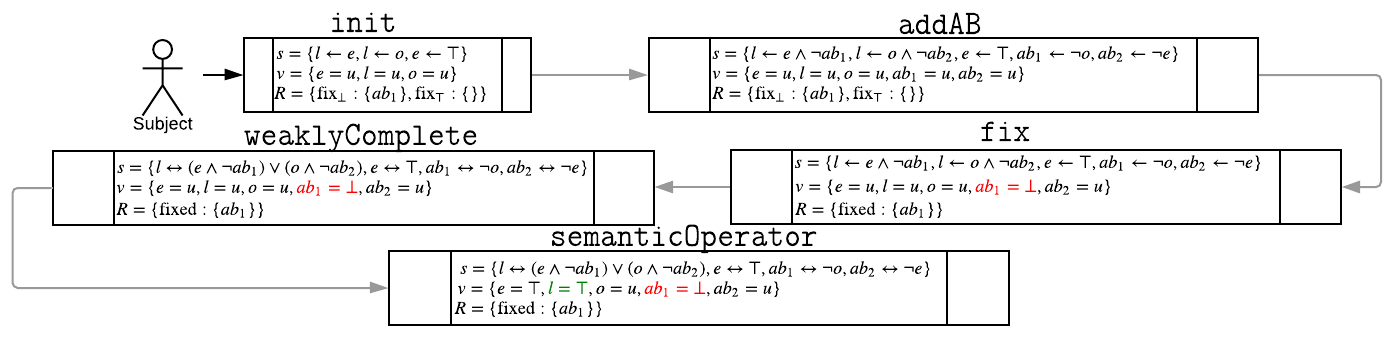
\includegraphics[width=\linewidth]{suppressionSCP_mod2}
\end{center}

\caption{The Suppression Task in which the additional operation of fixing the variable $ab_1$ to false occurs.}
\label{fig:supmod2}
\end{figure*}

The second case of a potential complex operation to add to the search space of our SCPs is the idea of Variable Fixing. The idea that some  conclusions can be fixed \textit{a priori}. Consider a person who strongly doubts the effectiveness of vaccines, we will call her Karen. Karen started her day convinced that giving her child the MMR vaccine is more dangerous than the disease itself. Later that day Karen spoke to her doctor who strongly advised that she vaccinate her child. He offered her a variety of peer-reviewed papers and studies that showed the relative safety of the vaccination. Karen listened carefully to the trained medical professional, and then went home. After some thought Karen decided that he was wrong, and her opinion on vaccines didn't change.

In this example Karen shows a very powerful type of cognitive bias, the unwillingness to change her opinions, despite powerful evidence to the contrary. This phenomenon has been observed across a great many fields of study, from medical psychology \citep{brown2010omission} \citep{wroe2005feeling} to political sciences\citep{tappin2017heart}. In the context of cognitive modelling with logics, it indicates that some mental rules or variables are immutable, regardless of new evidence or valid beliefs that would logically contradict them. Non-monotonic logics, as a class, are already capable of dealing with bias effects, as non-monotonic logics are built on the basis of a preference operation.

 As one possible implementation of this idea, let us introduce a cognitive operation called \texttt{fix}. Fix takes as input any state point and is applicable for any ground point $\bar{p}$ with variable list $V \in \bar{p}$ and categorization variable $R$ with ($fix_\top \lor fix_\bot) \in R$. For all variables $v$ such that $(v \in V) \cap (v \in fix_\top)$ set the value of $v$ to $\top$, For all variables $v$ $(v \in V) \cap (v \in fix_\bot)$ set the value of $v$ to $\bot$. Then remove $fix_\top$ and $fix_\bot$ from $R$. Append $fixed:V_{fix}$ to $R$, where $V_{fix}$ is the set of all variables fixed in this way.

Now, because \texttt{semanticOperator} does not change the values of variables mentioned in $V_{fix} \in fixed:V_{fix}$, $fixed \in R$, Figure~\ref{fig:supmod2} shows the effect of adding a complex operation which fixes the value of the abnormality to false in $v$ so that, no matter what rules in $KB$ when the semantic operator is applied, $ab_1$ will remain false.
\section{Wason Selection Task}
\chapter{Comparing SCPs} \label{chp:comparing}
\section{Why do we need to compare SCPs?} \label{sec:whyCompare}
The ability to compare the feasibility of different solutions is an essential step in any computational process in which multiple approaches produce the desired output. Consider a toy example of an SCP task which describes the mental process needed to bake a cake:

\[
\Pi = (s_0, M, \gamma, f())
\]

\[
s_0 = (V=(cakeBaked: \bot) )
\]
\[
M=\{\texttt{mixIngredients}, \texttt{bakeIngredients}, \texttt{doTheLaundry}\}
\]

\[
f(x)= \left\{ \begin{matrix} cakeBaked \models \top & & & \textrm{True}\\ cakeBaked \models \bot & & & \textrm{False} \end{matrix} \right\}
\]

\[
\gamma  = True
\]

Without specifying the precise details of the complex operations in $M$, and simply using our intuition of the effects of these actions, we can draw some candidate SCPs. Candidate SCPs such as $\mu=(\pi=(s_0 \longmapsto \texttt{mixIngredients}), f())$ do not result in the cake being baked and so are discounted immediately. However, consider a case where the modelling algorithm being used has come up with two possible SCPs to explain the processes chosen by the participant:

\begin{equation} \label{eq:bakeCake}
\mu_1 = (\pi_1=(s_0\longmapsto \texttt{mixIngredients} \longmapsto \texttt{bakeIngredients}),f())
\end{equation}

\begin{equation} \label{eq:bakeCakeLaundry}
\mu_2 = (\pi_2 = (s_0 \longmapsto \texttt{mixIngredients} \longmapsto  \texttt{doTheLaundry} \longmapsto \texttt{bakeIngredients}),f())
\end{equation}

Intuitively, both of these operational sequences would result in a cake being baked and both $f(\pi_1)\models \gamma$ and $f(\pi_1)\models \gamma$. Thus, both are candidate solutions to the SCP task given. However, both of these solutions may not be equally \textit{plausible}. Why would someone need to do their laundry to make a cake? We can concoct wild scenarios in which the participant's house is so full of dirty laundry that access to the oven it restricted, but this seems implausible. Most readers would agree that Equation~\ref{eq:bakeCake} is more plausible that Equation~\ref{eq:bakeCakeLaundry}.

This toy example is evidence that, in at least some cases, one can confidently prefer one SCP to another. The question now arises: how do we precisely, and consistently prefer one SCP over another? This question is not easy to answer, and this chapter is devoted to proposing candidate solutions which may be able to quantitatively score and select preferable SCPs.

Section~\ref{ssec:compGen} discusses the question of how to compare different SCPs found using search for a single task. Section~\ref{ssec:compExt} discuses the more general problem of comparing SCPs even when the underlying SCPs tasks differ. Section~\ref{ssec:nw} introduces the Needleman-Wunsch Algorithm for string matching whose underlying principles have allowed us to quantify questions of homology and evolutionary relationships in biology.

\section{Comparing Generated SCPs} \label{ssec:compGen}
\subsection{Scoring}
Cognitive modelling as a science that exists, in part, to replicate the empirical results of human reasoning suffers from a painful truth: just because a solution is simple, elegant and seemingly well-justified, it does not follow that that solution is correct. Indeed, that solution might completely fail to explain experimental data from a cognitive task, and must then be discounted. However in the fields of string-matching, etymology, and homological evolution \citep{sweetser1990etymology} \citep{needleman1970general} , mathematically consistent approaches to scoring are still generally a good starting point. And so we carry that assumption into the field of cognitive modellings and assume that, in the absence of directly contradictory empirical data, certain properties related to finding the optimal sequence of cognitive operations are desirable, whilst others are not.

In general the easiest way to compare two distinct objects is to quantify some subset of their properties and use these properties to rank the objects. Continuing with the toy example in Section~\ref{sec:whyCompare} we will attempt to create a commonsense scoring mechanism to determine whether $\mu_1$ or $\mu_2$ is a more cognitively plausible solution to baking a cake. A great many possible criteria exist for scoring these two SCPs, but we will focus on just two of them: the length of the SCP, and the plausibility of each cognitive operation that occurs in either SCP.

\subsubsection{SCP Length}
Perhaps the simplest and most intuitive way to decide which of two SCPs is best suited to solving a specific problem is to prefer the shortest one. In the field of Bioinformatics, one of the earliest approaches to determine which two organisms from a set were more closely related was to directly estimate how many genetic mutations (insertions, deletions, value changes) would be necessary to turn each of these genetic sequences into each other sequence. The same logic can be applied to SCPs for those SCPs generated using either \textit{De Novo} or \textit{Insertion Search} (Section~\ref{ssec:scpSearch}).

If we define the length $|\mu|$ of an SCP $\mu=\{\pi,f()\}$ to be number of cognitive operations present in $\pi$. In the case of \textit{De Novo} search, we assume assume that the optimal length of a solution to $\Pi$ is an SCP $\mu^*=(\pi^*,f())$ with length $|\mu^*|=0$. This optimal solution obviously does not exist in this case $f(s_0) \not\models (cakeBaked = \top)$, but it serves as a way of implicitly preferring shorter SCPs, as those will require fewer insertion operations to satisfy $f(x)$. 

Using this simple test criteria: $|\mu_1| < |\mu_2|$, therefore $\mu_1$ is preferred because it requires only $2$ operations to transform the ideal SCP $f(s_0)$ into $f(s_0\longmapsto \texttt{mixIngredients} \longmapsto \texttt{bakeIngredients})$, rather than the $3$ required for $mu_2$.

Though simple, this scoring procedure provides the foundations upon which more complex scoring algorithms will be built for the remainder of this section.

\subsubsection*{Limitations}

Unfortunately, the SCP Length approach fails to capture anything about the \textit{relationship} between the SCPs being scored. Let us examine the following three SCPs, all generated whilst modelling the Wason Selection Task:
\[
\pi_\text{WST}=(s_{WST} \longmapsto \texttt{addAB} \longmapsto \texttt{addExp} \longmapsto \texttt{wc} \longmapsto \texttt{semantic})
\]
\[
\pi_\text{prop}=(s_{WST} \longmapsto \texttt{th})
\]
\[
\mu_{D,3}=(\pi_{WST},f_\text{WST}())
\]
\[
\mu_{D,7}=(\pi_\text{WST},f_\text{WST}^\text{pref}())
\]
\[
\mu'_{D,7}=(\pi_\text{prop},f_\text{WST}^\text{pref}())
\]

Using SCP Length, $|\mu_{D,7}|=4$ and $|\mu'_{D,7}|=1$ and we would would conclude that $|\mu'_{D,7}|=1$ is the more probable SCP.

In isolation, given only $|\mu_{D,7}|$ and $\mu'_{D,7}$, this conclusion makes some sense. $\mu'_{D,7}$ is indeed significantly shorter, and can be achieved with a single cognitive operation. But our information about these SCPs comes with more context than that. Assume that we are certain that $\mu_{D,3}$ is an accurate model for some other related cognitive task. Now it seems plausible that the solution to a related cognitive task may be an offshoot of an underlying core process. From this perspective, if we belief that $\mu_{D,3}$ has an underlying model in common (save for some `mutations' which add or remove cognitive operations) with the solution to the task to turn the $D$ and $3$ cards, $\mu_{D,7}$ seems significantly more likely than $\mu'_{D,7}$.

\section{Comparing External SCPs} \label{ssec:compExt}

One of the core principles of biological scoring algorithms is the intuition that the genetic structures being analysed share a common ancestor at some point in the post. With this assumption it becomes possible to model precisely what genetic mutations one sequence might have undergone to become the other.

This intuition carries surprisingly well into the field of cognitive modelling where researchers very often search for common core mechanisms shared between different reasoners, or across different cognitive tasks. Concepts like the Diversity Principle\citep{heit2005defending}, and denial of the antecedent are often shown be powerful predictors of participant responses.

To this end, I propose that the concept of a shared underlying cognitive process in cognitive modelling can be considered analogous to the concept of shared ancestry in genetic sequences. If we assume that the SCP Framework is a valid mechanism for human cognition, it becomes possible to use these biological principle to compare and score SCPs.

\subsection{The Needleman-Wunsch Algorithm} \label{ssec:nw}

\begin{table}
\begin{center}

\begin{tabular}{ c c c}
 \textbf{Event}&\textbf{Process} & \textbf{Score} \\ 
 \hline
 $x=y$ & Match & 1 \\
 $x\neq y$, $x \neq $`-', $y \neq $`-' & Mismatch & -1 \\
 $x=$`-',& Insert & -1 \\
 $y=$`-'& Delete & -1
\end{tabular}
\caption{A very simple table for scoring SCPs with the Needleman-Wunsch algorithm for inputs $x$ and $y$.}
\label{tbl:simpleneed}

\end{center}
\end{table}

\begin{table}
\begin{center}
\begin{tabular}{c | c c c c c c c }
 & & A & T & T & A & C & A\\
 \hline
 & 0 & -1 & -2 & -3 & -4 & -5 & -6\\
A & -1 & 1 & 0 & -1 & -2 & -3 & -4\\
T & -2 & 0 & 2 & 1 & 0 & -1 & -2\\
G & -3 & -1 & 1 & 1 & 0 & -1 & -2\\
C & -4 & -2 & 0 & 0 & 0 & 1 & 0\\
T & -5 & -3 & -1 & 1 & 0 & 0 & 0
\end{tabular}
\caption{Scoring matrix for the sequences $a=ATTACA$ and $b=ATGCT$ using the scoring properties defined in Table~\ref{tbl:simpleneed}.}
\label{tbl:NW_nucleotides}
\end{center}
\end{table}


In the field of Bioinformatics, one of the earliest approaches to determine which two organisms from a set were more closely related was to directly estimate how many genetic mutations (insertions, deletions) would be necessary to the genetic sequence of one of those animals into the other. \cite{needleman1970general} proposed a simple scoring algorithm to determine how similar two genetic sequences were to one another by computing how many insertions, deletions, and mutations the first sequence would have to undergo to become the second sequence, and assigned a quantitative penalty or reward to each of these events. 

Needleman's recursion makes use of a dynamic programming approach and \textit{score matrix} $D$ to score two sequences efficiently ($O(nm)$ time and $O(nm)$ space complexity for sequences of length $n$ and $m$, respectively). The recursion for his algorithm for sequences $a$ and $b$ is as follows:
\[
D_{0,j}=\text{insertion cost} \times j
\]
\[
D_{i,0}=\text{deletion cost} \times i
\]
\[
D_{i,j}=\text{min}
\begin{pmatrix}
D_{i-1,j-1} & + & s(a_i,b_j)\\
D_{i-1,j} & + & s(a_i, - )\\
D_{i,j-1} & + & s(-,b_j)
\end{pmatrix}
\]
Where an example of the costs $s(x,y)$ is given by Table~\ref{tbl:simpleneed}. Matches are usually positively scored (desirable), and mismatches, insertions, and deletions, are usually negatively scored (undesirable).

Needleman also defined a traceback algorithm to show what this optimal global alignment was. The traceback begins at the bottom right corner of the $D$ matrix and for, position $D_{i,j}$, calculates which neighbouring value $D_{i-1,j-1}$, $D_{i-1,j}$, $D_{i,j-1}$ would result in $D_{i,j}$ when added to the cost of match/mismatch, insertion and deletion respectively. We will not detail this aspect of the algorithm beyond this point because our interest lies in the scoring itself, rather than the traceback.

Table~\ref{tbl:NW_nucleotides} shows the scoring matrix for the sequences $a=ATTACA$ and $b=ATGCT$, and the optimal alignment is given by:
\[
\begin{pmatrix}
A & T & T & A & C & A \\
A & - & T & G & C & T
\end{pmatrix}
\]
Where $-$ denotes an insertion or deletion.

\subsubsection{Needleman-Wunsch for SCPs}

\begin{table}
\begin{center}
\begin{tabular}{c | c c c c c c }
 & & $s_\text{WST}$ & addAB & addExp & wc & semantic\\
 \hline
 & 0 & -1 & -2 & -3 & -4 & -5\\
$s_\text{WST}$ & -1 & 1 & 0 & -1 & -2 & -3\\
addAB & -2 & 0 & 2 & 1 & 0 & -1\\
addExp & -3 & -1 & 1 & 3 & 2 & 1\\
wc & -4 & -2 & 0 & 2 & 4 & 3\\
semantic & -5 & -3 & -1 & 1 & 3 & 5
\end{tabular}
\caption{Needleman-Wunsch comparison of $\mu_{D,3}$ to $\mu_{D,7}$}
\label{tbl:compD3D7}
\end{center}
\end{table}

\begin{table}
\begin{center}
\begin{tabular}{c | c c c c c c }
 & & $s_\text{WST}$ & addAB & addExp & wc & semantic\\
\hline
 & 0 & -1 & -2 & -3 & -4 & -5\\
$s_\text{WST}$ & -1 & 1 & 0 & -1 & -2 & -3\\
th & -2 & 0 & -1 & -2 & -3 & -4
\end{tabular}
\caption{Needleman-Wunsch comparison of $\mu_{D,3}$ to $\mu'_{D,7}$}
\label{tbl:compD3D7prime}
\end{center}
\end{table}

The initial extension of the Needleman-Wunsch algorithm to the SCP framework is surprisingly simple. Because known SCPs are guaranteed to consist of a linear, finite sequence of cognitive operations, and comparison between cognitive operations is possible (two cognitive operations are equal if they have the same name), the only thing the SCP framework lacks is a way to represent insertions and deletions. To this end we define the \texttt{insert} cognitive operation. 

\begin{algorithm}[H] \label{cogOp:insert}
\SetAlgoLined
\SetKwProg{Fn}{Function}{ is}{end}
\Fn{$e$($\bar{p}$)}
{
\Return $\bar{p}$
}

\caption{\texttt{insert}$(\bar{p})$: an empty cognitive operation used as a place-holder for scoring.}
\end{algorithm}

Like the $\texttt{th}$ operation, \texttt{insert} has no function in an SCP Task, and is not assumed to be a function with an analogue in human reasoning. Instead it is a placeholder function that represents some unknown function in the shared cognitive process from which both SCPs are assumed to originate.

Finally, we must decide how the initial epistemic state is to be scored. For now we will simply treat the $s_i$ as if it were a cognitive operation for scoring purposes.

Now we can compare out candidate solution SCPs $\mu_{D,7}$ and $\mu'_{D,7}$ using the score system from Table~\ref{tbl:simpleneed} and the Needleman-Wunsch Algorithm. Table~\ref{tbl:compD3D7prime} shows global alignment score of -4 for ($\mu_{D,3}$,$\mu'_{D,7}$), whereas Table~\ref{tbl:compD3D7} has a global alignment score of 5 for ($\mu_{D,3}$,$\mu_{D,7}$) and so $\mu_{D,7}$ is believed to be more similar to $\mu_{D,3}$.
\[
\text{align}(\mu_{D,3},\mu'_{D,7}) =
\begin{pmatrix}
s_\text{WST} & \texttt{addAB} & \texttt{addExp} & \texttt{wc} & \texttt{semantic} \\
s_\text{WST} & \texttt{addAB} & \texttt{addExp} & \texttt{wc} & \texttt{semantic}
\end{pmatrix}
\]
\[
\text{align}(\mu_{D,3},\mu_{D,7}) =
\begin{pmatrix}
s_\text{WST} & \texttt{addAB} & \texttt{addExp} & \texttt{wc} & \texttt{semantic} \\
s_\text{WST} & \texttt{insert} & \texttt{insert} & \texttt{insert} & \texttt{th}
\end{pmatrix}
\]
It is my belief that this technique offers a great deal of insight into which cognitive operations are to be prefered, and, over a sufficiently large number of well-founded SCPs for different cognitive tasks, may help to shape our future theories about what general processing motifs really inform certain aspects of human cognition.

\subsubsection{Extending Needleman-Wunsch for SCPs}

We have now seen that SCP similarity can be computed using the Needleman-Wunsch algorithm. \texttt{SCP\_ scoring\_ improved} in the implementation of the SCP framework takes this approach one step further and assigns unique scores to matches, mismatches, and insertion operations for every cognitive operation. This allows the researcher to specify intuition about the relative complexity of each cognitive operation. 

I will not detail this approach further in this thesis because I do not currently have an intuition as to how these scores should be calculated for each operation, but it is worth noting that the implementation exists.

\subsection{Limitations of the Needleman-Wunsch Algorithm}

The Needleman-Wunsch algorithm is generally considered a good introductory algorithm to those learning bioinformatics, but it lacks many of the useful features of more advanced algorithms in the field. In a similar way, it was used here to show the suitability of similarity scoring algorithms to SCPs, logical extensions to more advanced string-matching algorithms are easily imagined.

A significant limitation of the Needleman-Wunsch algorithm, and by extensions our algorithm, is the inability to deal with crossovers. That is, the algorithm cannot handle cases where operators or groups of operators are shifted into a new position (imagine cutting the middle out of a piece of string and retying it to the end of the string). This limitation is imposed by many such algorithms to limit the computational complexity of the computation, without this limitation string matching becomes NP-hard.

The Smith-Waterman algorithm \citep{smith1981identification} is a simple variation on the Needleman-Wunsch algorithm and is used to  find optimal local alignments. It could be used to find subsequences of complex actions that are preserved between different SCPs. These subsequences (for example the pCTM $(\texttt{addAB} \longmapsto \texttt{wc}$) may be shown to be present in comparisons of models of different cognitive tasks, and may be considered to show support for common motifs in general human cognition.


\chapter{Program Design} \label{chp:program}
\section{Implementing the SCP Framework}
The SCP framework has been implemented in \texttt{Python 3} as series of modules which follow strong object-oriented programming principles which support simple extensions and revisions. This implementation is used to demonstrate the practical approaches to generating and evaluating SCPs; and to model a series of cognitive tasks for which empirical results already exist. The library containing this implementation and its associated documentation is available at @TODOref.

At present, concrete implementations for epistemic state structures and cognitive operation formulations related to propositional logic, the WCS, and Reiter's default logic are provided.

\section{A Modular Programming Approach}
% talk about each 
The principle of modular programming is followed in this implementation to the greatest extent possible, thus maximising the ease of modification and upkeep for the program. Figure~\ref{scpClassDiagram} provides a simplified class diagram to explain how the major components of the system relate to one another.

\subsection{Most Important Modules}

\begin{figure}
\centering 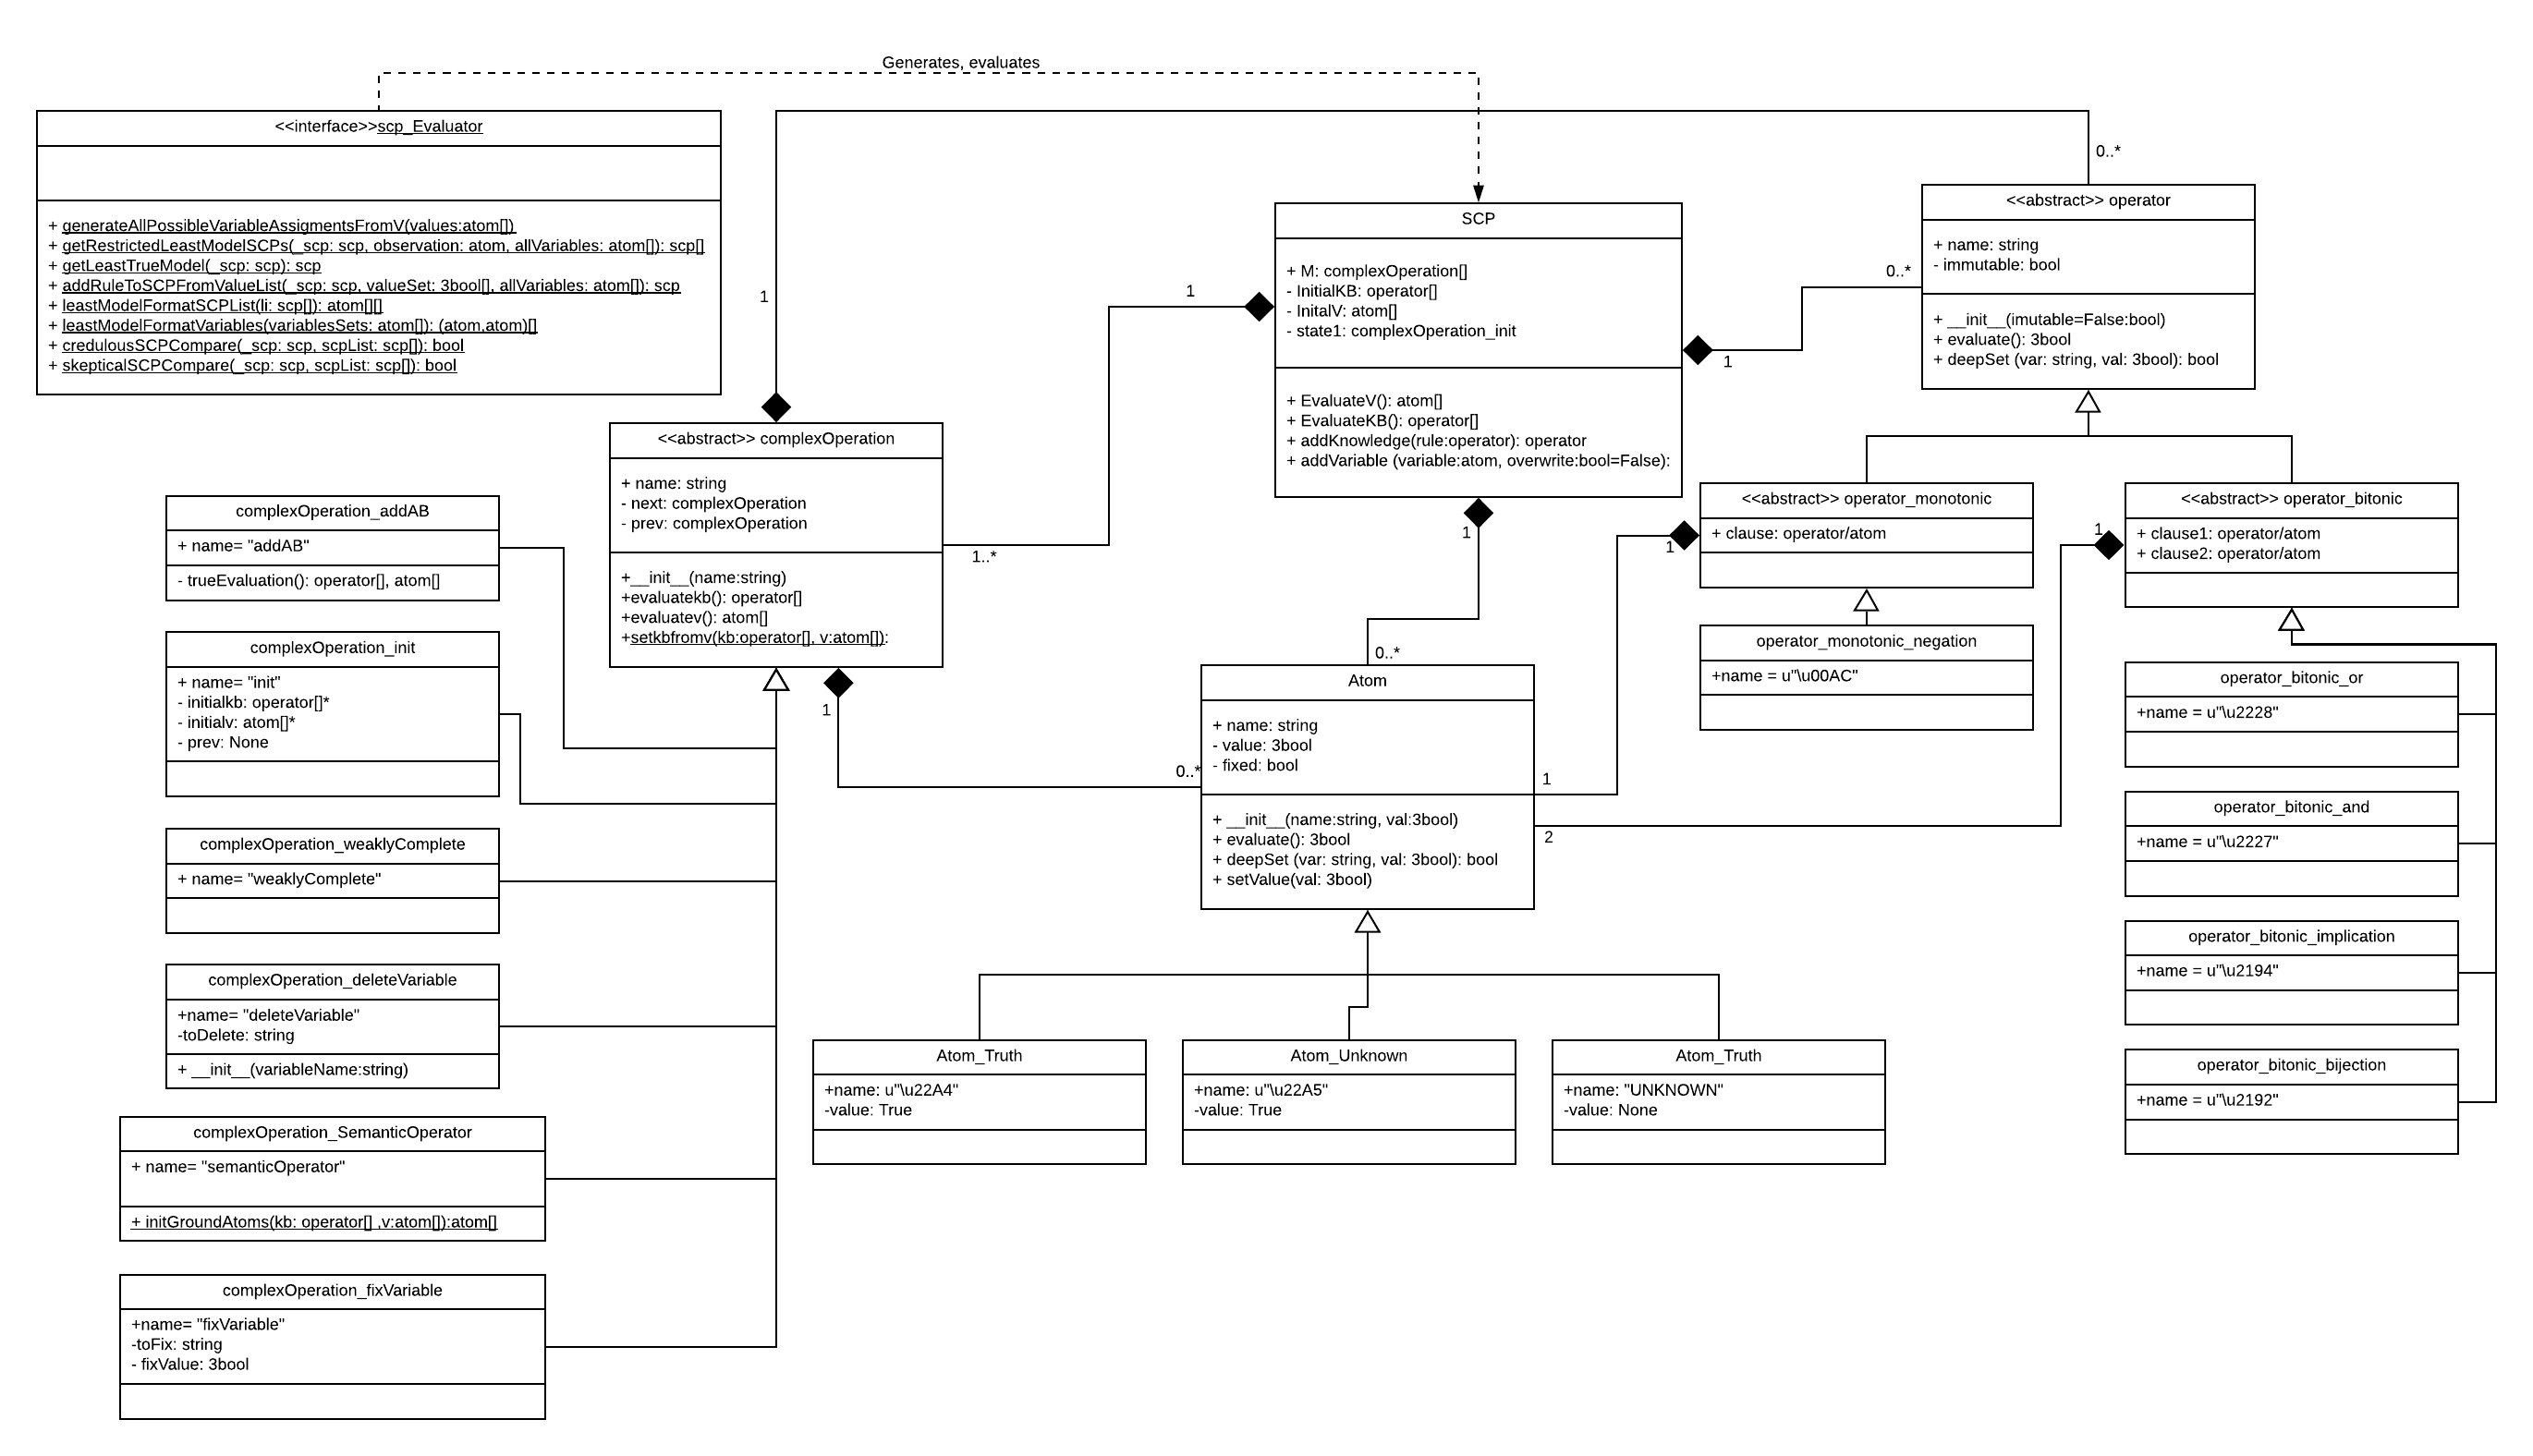
\includegraphics[width=\linewidth]{scpClassDiagram}
\caption{Class diagram for the implementation of the SCP Framework.}
\label{fig:scpClassDiagram}
\end{figure}

\begin{itemize}
\item $\texttt{basicLogic}$: an implementation of basic two and three-valued logic.
\item $\texttt{SCP\_Task}$: implements both the SCP Task ($\Pi$) object and a search function for generating SCPs which meet the given goals.
\item $\texttt{CTM}$: implements the CTM $\pi$ and defines the $J[p,m]$ application of a cognitive operation to an input state point
\item $\texttt{CognitiveOperations}$: defines the set of cognitive operations as well as the their input and output parameters.
\item $\texttt{StatePointOperations}$: defines $f(\pi) \models_\text{strict} \gamma$ and $f(\pi) \models_\text{weak} \gamma$ determining if a given SCP meets a given set of output criteria.
\item $\texttt{truthTables}$: a set of truth tables for each operator defined in \texttt{basicLogic}.
\item $texttt{SCP\_scoring}$: an implementation of the Needleman-Wunsch Algorithm for SCPs described in Chapter~\ref{chp:comparing}
\item $texttt{SCP\_scoring\_extending}$: an implementation of the extended Needleman Wunsch Algorithm for SCPs described in Chapter~\ref{chp:comparing}
\end{itemize}

\subsection{Program Flow}
\begin{figure}
\centering 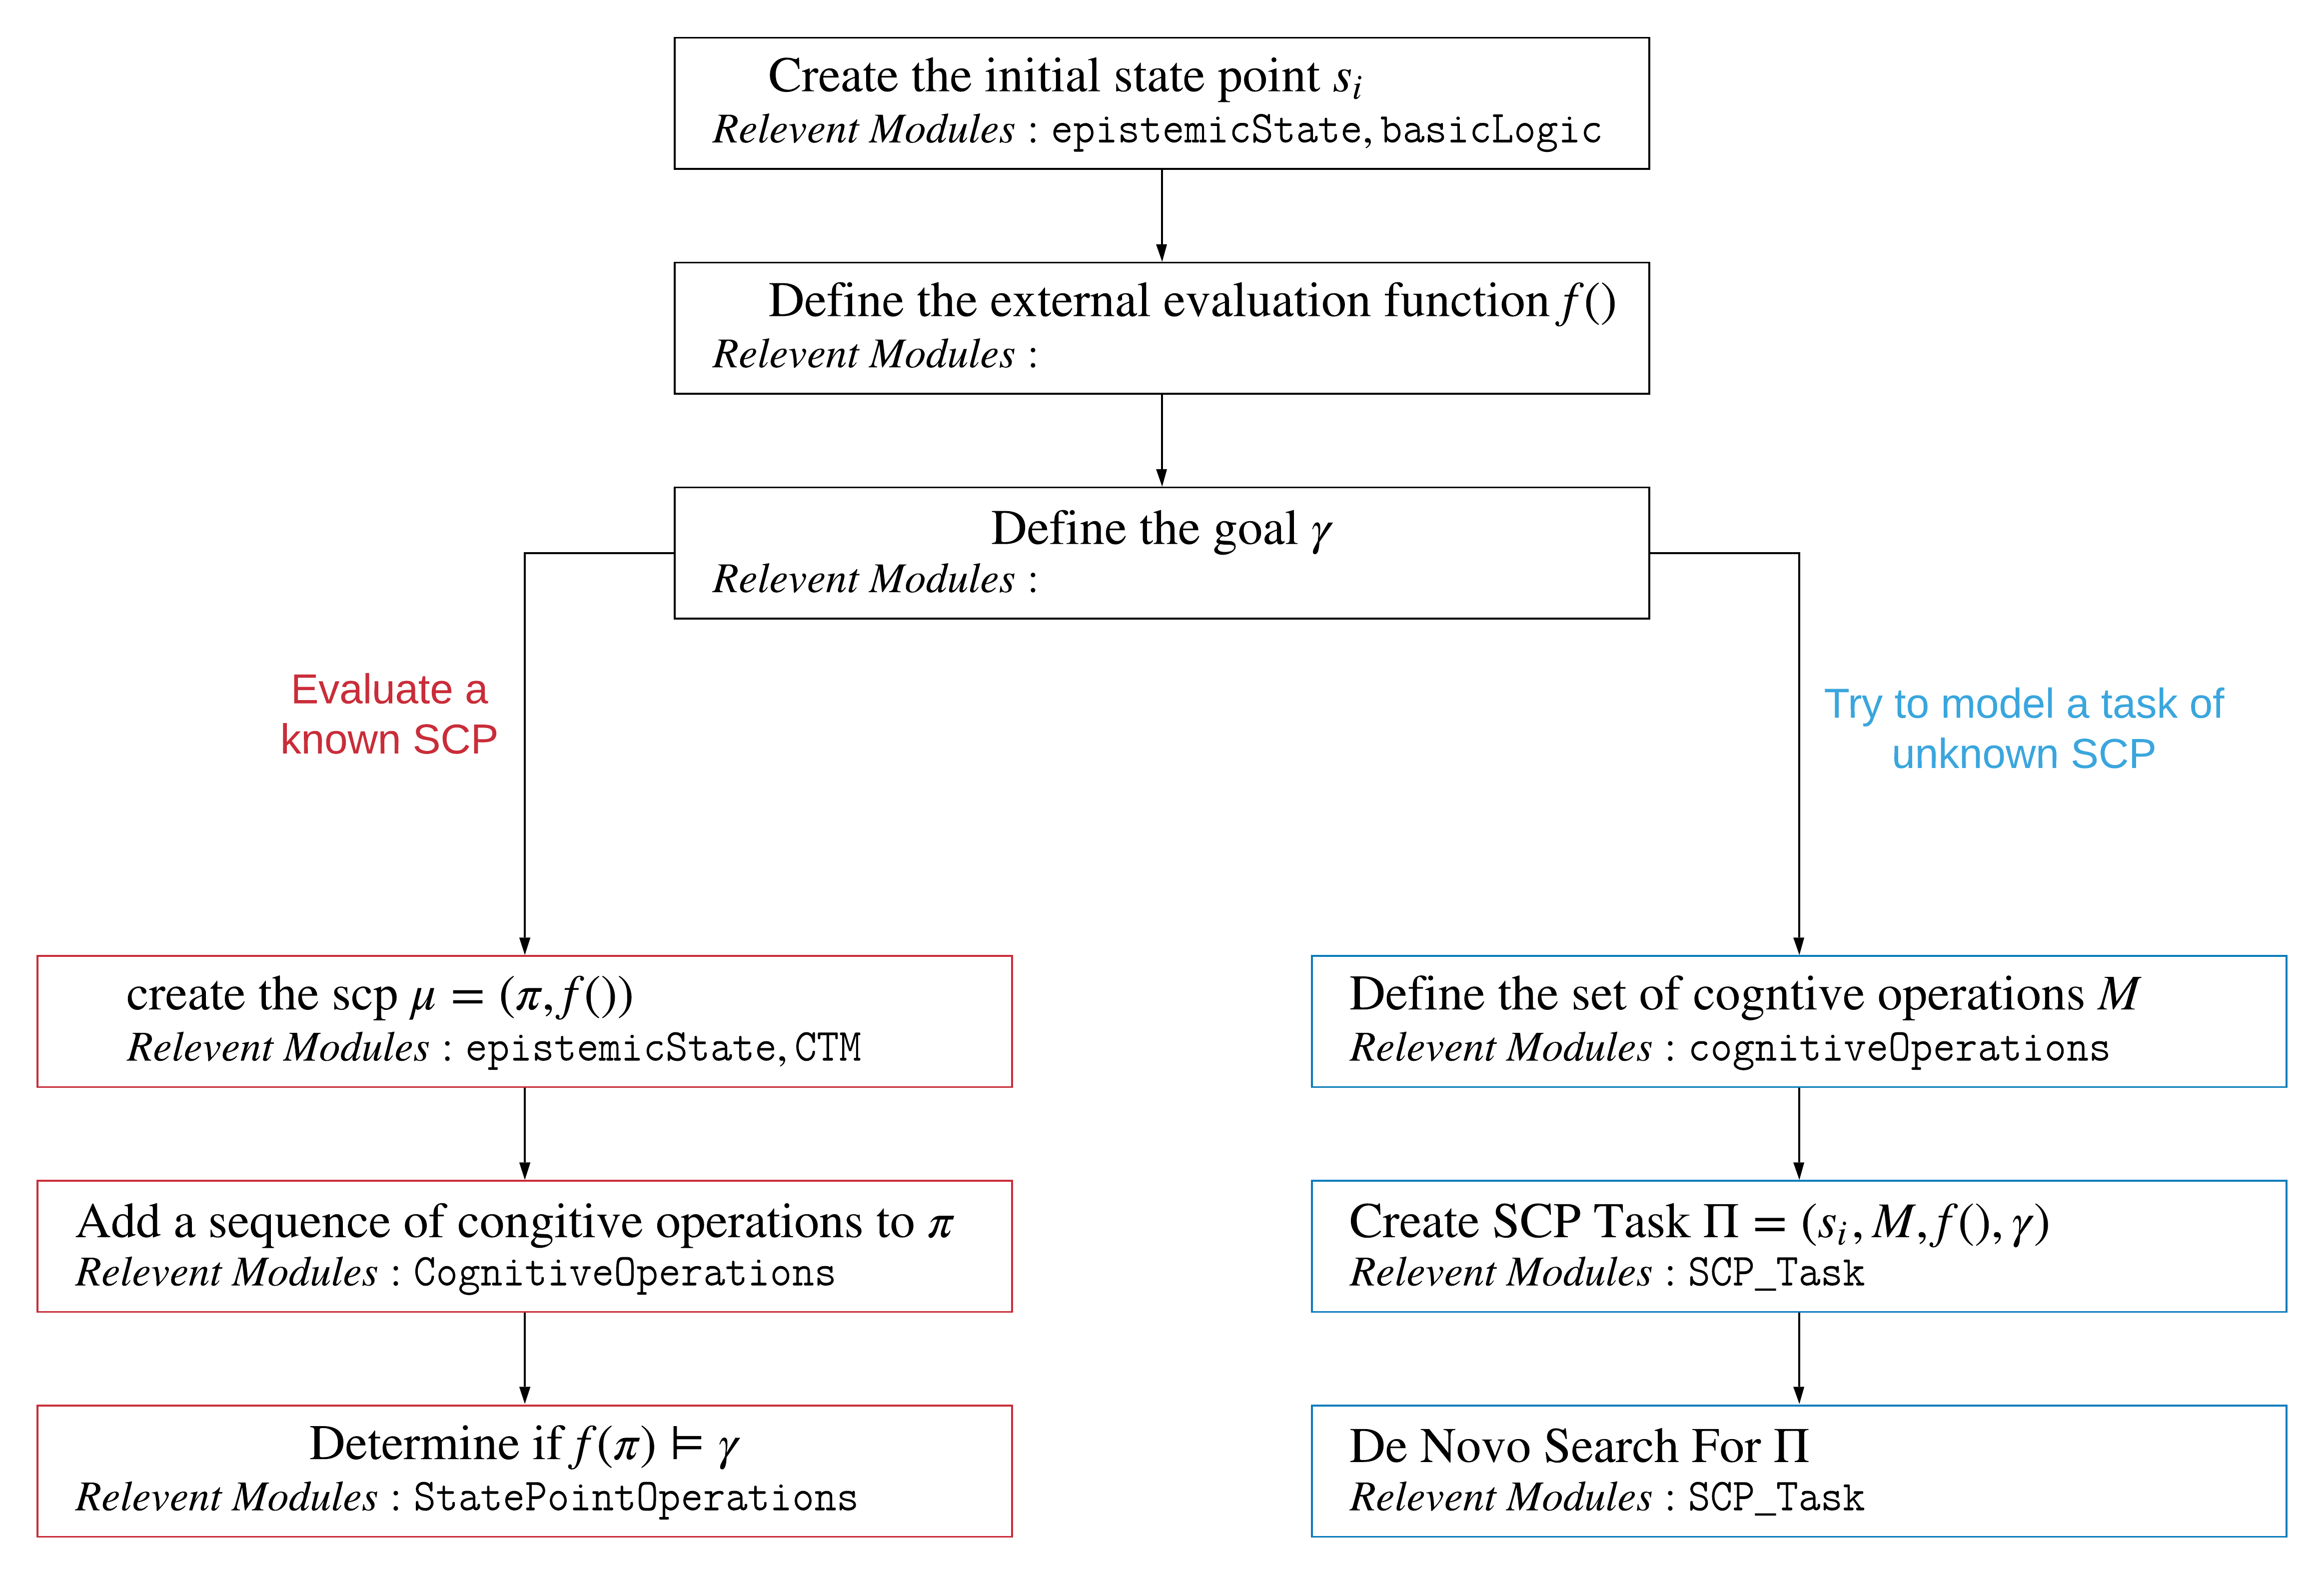
\includegraphics[width=\linewidth]{SCP_Use_Cases}
\caption{Two use cases for the implementation of the SCP framework}
\label{fig:SCP_Use_Cases}
\end{figure}



Diagram~\ref{fig:SCP_Use_Cases} illustrates the basic programmatic flow used to model either a known SCP or known empirical result set using the SCP Framework. In the appendix, Figure~\ref{fig:sup_snippet} provides a code snippet to show exactly how the general case of the Suppression Task is modelled in the SCP framework.



\subsection{Modelled Experiments}
\begin{itemize}
\item \texttt{suppressionTask.py}: models the Suppression Task as discussed in Chapter~\ref{chp:model}.
\item \texttt{WST.py}: models the Wason Selection Task as discussed in Chapter~\ref{chp:model}.
\end{itemize}

\section{External Framework Integration}
At present work is ongoing to integrate the SCP framework with \texttt{CCOBRA} \citep{ccobra}.














%\chapter{Non-Sequential Cognitive Processes} \label{chp:nscp}
% relation to neural networks
% summarising tool
\section{Overview}
The SCP framework has already been shown to be a powerful tool for modelling human cognition across a number of tasks, but as a framework it still carries several limitations. The first and most significant of which is the requirement that only one state point is passed as input and one state point is produced as output. This requirement ensures that a linear formulation of the SCP is possible and an intuitive procession of cognitive operations is apparent. SCPs are also limitted to representing or describing only a single cognitive task's interpretation by only a single or generalised reasoner. These properties are desirable when attempting to explicitly model a specific response to with relation to empirical data, but to model a group of reasoners with disparate responses, a group of SCPs is required.

By relaxing the requirement that every SCP outputs into one other cognitive operation we arrive at new type of cognition process, a \textit{non-Sequential Cognitive Process} (\textit{nSCP}). nSCPs are more powerful than traditional SCPs and can produce process models for different reasoners over a task using a single SCP. They also provide a mechanism for illustrating motif reuse across multiple cognitive tasks which can all be modelled using the same nSCP. Finally, nSCPs lend themselves well to machine learning techniques, and graph compression approaches, allowing researchers to derive minimal inter and cross-task models.

\section{Applications}

\section{nSCPs: a Formal Framework}

\section{The Suppression Task as an nSCP}

Figure~TODOref showed one possible SCP interpretation of the Suppression Task that satisfied the empirically observed general case of the task. Figures~@TODOref and @TODOref showed two possible SCPs that described the deviant `classical' response to the task using non-monotonic logics. These three disparate representation can be compared to one another using the techniques described in Section~@TODOsec using the proposed modified Needleman-Wunsch algorithm, but these quantitive comparissons do not intuitive illustrate the structural similarity between these three SCPs.

Figure~@TODOref shows an nSCP constructed so that any of the possible individual SCP paths can be followed. This, more compact approach carries the desirable property of colapsing the motifs @TODOlistmotifs into shared structures thus reducing the total number of distinct cognitive operations needed represent the task by @TODOxPrecent. 

\section{The Wason Selection Task as an nSCP}


\section{A cross-task nSCP}

\section{Multiple Inputs with an nSCP}
Sometimes the information we use in reasoning comes from various distinct cognitive data structures @TODOref and, therefore are plausibly produced by differing prior cognitive processes.

Consider the following two facts a person may have been afflicted with due to an unfortunate surplus of education:
\begin{itemize}
\item ``Those who speak Greek come from Greece."
\item ``Aristotle speaks Greek."
\end{itemize}



A person might have this information in their background knowledge about the world.  This person might then decide to take part in a cognitive experiment and be presented with a new incomplete syllogism:

\begin{itemize}
\item ``All men are mortal."
\item ``Aristotle is a man."
\end{itemize}

And be asked what conclusions they could draw from the following statement:

``Mortals who are Greek believe in Zeus."

By \textit{combining} their background knowledge about syllogism~@TODOref with the presented knowledge about the second syllogism the reasoner might derive two, chronologically distinct facts:

\begin{itemize}
\item From the new information: ``Aristotle is mortal"
\item From relevant background knowledge: ``Aristotle Speaks Greek".
\end{itemize}

These two derived facts are both relevant to the question being asked, but are drawn from distinct information sources. In a standard SCP for propositional logic we would be forced to combine the two facts into a single knowledge base (removing contextual information about information that might be relevant in human reasoning), create a new epistemic state structure that explicitly captures marks the background and task-specific knowledge as distinct rule sets, or to pre-process background knowledge before adding it to the given knowledge.

An nSCP framework offers a fourth, more elegant, solution that captures the spirit of the pre-processing approach. Because an nSCP can take multiple cognitive operations as inputs, it is possible to attach two seperate cognition trees - one of background knowledge and one for given knowledge - to one another and use an \textit{integrating operation} to combine their outputs into a single epistemic state.

Figure~TODOref illustrates one possible formulation of our example as an nSCP where @TODO is an integrating operation which uses the following rule: @TODO.

\section{Machine Learning with nSCPs}

nSCPs have a structure which many people experienced with machine learning will recognise. 


\chapter{Conclusions and Future Work} \label{chp:conclusion}
\section{Conclusion}
This thesis has introduced, and implemented, a new computational framework into the field of cognitive modelling which is able to capture much of the nuance of other non-monotonic frameworks, whilst still maintaining a consistent technique for task formulation and evaluation. 

Over the course of this thesis we have: introduced three levels of granularity into the description of cognitive tasks by formalising the mathematical structure of SCP Plans, SCPs, and Realised SCPs; established a viable search procedure for generating new SCPs from SCP Tasks; defined a set of cognitive operations that can be used for modelling both general and individual case of the Wason Selection Task and Suppression Task using the Weak Completion Semantics; shown that the intuition and functionality of both the WCS and Reiter's Default Logic can be encoded using the SCP framework; modelled the WST and Suppression Task using entirely novel approaches for both the general and individual reasoner; established both theoretical and empirical evidence for SCPs as models of human cognition; and implemented a robust scoring system for comparing SCPs under the assumption that they both represent deviations from an underlying cognitive process.

SCPs represent a novel and powerful framework for modelling non-monotonic logics. They have been shown capable of modelling the Suppression Task and Wason Selection under the WCS for both general and individual cases. SCPs provide a dynamic framework incorporating cognitive operations which are applicable across different logics, provided that those logics share structural features that are compatible with some subset of the known set of cognitive operations. Because the input and output epistemic states need not be structurally similar, SCPs may represent the first approach to modelling human cognition that is able to integrate multiple non-monotonic logic frameworks at run-time and at search-time. 

SCPs represent a new frontier for Cognitive Modelling in non-monotonic logics and research into their capabilities and limitations may help create more robust and mathematically consistent explanations and predictions for human behaviour across an extensive array of cognitive tasks.

\section{Future Work}

One of the most obvious extensions of the SCP framework, is the creation of cognitive operations which are able to model first-order logical systems, rather than the propositional systems to which this thesis has been restricted. The introduction of techniques from machine learning, artificial intelligence planning and reinforcement learning would allow for several desirable extensions of the SCP Framework, including but not limited to: more empirically well-founded score tables when comparing SCPs, the generation of heuristic techniques to search through SCPs and SCP Plans with large branching factors, and the development of techniques to generate novel cognitive processes which are evidenced in SCPs across different cognitive tasks. From a more theoretical outlook, formal properties of SCPs which combine techniques from several cognitive models should be identified and described. From a practical perspective, integration of the implemented SCP framework with existing modelling tools like CCOBRA will make the framework far more accessible to researchers who wish to generate models for observed cognitive phenomena. 



%----------------------------------------------------------------------------------------
%	THESIS CONTENT - APPENDICES
%----------------------------------------------------------------------------------------

\appendix % Cue to tell LaTeX that the following "chapters" are Appendices

% Include the appendices of the thesis as separate files from the Appendices folder
% Uncomment the lines as you write the Appendices

%----------------------------------------------------------------------------------------
%	BIBLIOGRAPHY
%----------------------------------------------------------------------------------------

\printbibliography[heading=bibintoc]

%----------------------------------------------------------------------------------------


\chapter*{Appendix} \label{chp:appendix}
\section*{Definitions and Proofs}
\begin{definition} \label{def:exp}
The expansion operation \textbf{exp} operation precisely substitutes a pCTM for its constituent elements as follows: 
\begin{enumerate}
\item Let $F$ be a pCTM such that: $F=(A \longmapsto B \longmapsto C)$, with $A \in \Omega^*$, $B \in \Omega^*$, $C \in \Omega^*$, and $B = (B_1 \longmapsto ... \longmapsto B_n)$, $B_i \in \Omega^*$. 
\item Then $F=(A \longmapsto \text{exp}(B) \longmapsto C)$ $=$ $(A \longmapsto B_1 \longmapsto ... \longmapsto B_n \longmapsto C)$/
\end{enumerate}
\end{definition}

\begin{definition} \label{lem:uniredundant}
Given a cognitive operation sequence $A \in \Omega^*$, a final state dependant external evaluation function $f()$, and goal $\gamma$, $A$ is \textbf{redundant} iff one of the following holds:
\begin{itemize}
\item $f(s_i \longmapsto \text{exp}(B) \longmapsto \text{exp}(C)) \models x'$ and $f(s_i \longmapsto \text{exp}(A)) \models x'$ for every viable epistemic state $x$, $B \in \Omega^*$, $C \in \Omega^*$, where neither $B$ nor $C$ is the empty set or the trivial operation $T$ (See Definition~\ref{def:exp}, for a definition of the exp operation). 
\item $f(s_i \longmapsto \text{exp}(A)) = f(s_i)$ for every viable state point $s_i$.
\item $f(s_i \longmapsto \text{exp}(B))=c$ for all $B \in \Omega^*$, where $c$ is constant.
\end{itemize}
\end{definition}

\begin{definition} \label{lem:taskredundant}
Given a limited set of cognitive operations $M=\{A_0, ..., A_n\}, A_i \in \Omega^*$, a final state dependant external evaluation function  $f()$, and goal $\gamma$, $A \in M^*$ is \textbf{task redundant} iff one of the following holds:
\begin{itemize}
\item $f(s_i \longmapsto \text{exp}(B) \longmapsto \text{exp}(C)) \models x'$ and $f(s_i \longmapsto \text{exp}(A)) \models x'$ for every viable epistemic state $x$, $B \in M^*$, $C \in M^*$, where neither $B$ nor $C$ is the empty set or the trivial operation $T$ (See Definition~\ref{def:exp}, for a definition of the exp operation). . 
\item $f(s_i \longmapsto \text{exp}(A)) = f(s_i)$ for every viable state point $s_i$.
\item $f(s_i \longmapsto \text{exp}(B))=c$ for all $B \in M^*$, where $c$ is constant.
\item There exists no sequences $B \in M^*$, $C \in M^*$, and state point $s_i$ such that $\mu=(\pi,f())$ is a valid SCP, with $\pi=\{s_i \longmapsto B \longmapsto A \longmapsto C)\}$.
\end{itemize}
\end{definition}














\begin{lemma}\label{lemma:monorealisedandback}
Let $\mu=(\pi,f())$ be a monotonic SCP, with $\pi=(s_i \longmapsto m_1 \longmapsto ... \longmapsto m_n)$, $m_i\in \Omega^*$. $r=(k \in K[\pi],f())$ is the only realised SCP of $\mu$, with $K[\pi]=\{s_i \longmapsto (m_1,\bar{p}_1) \longmapsto ... \longmapsto (m_n,\bar{p}_n)\}$, and for every pair $(m_i,\bar{p}_i)$, $\bar{p}_i \in_s J[\bar{p}_{i-1},m_i]$. Then it is trivially easy to derive $\mu$ from $r$, and \textit{vice versa}.
\end{lemma}

\begin{bulletProof} \label{proof:monorealisedandback}
\begin{itemize}
\item Determining $r$ from $\mu$:
\begin{itemize}
\item Let $R'=\{k \in K[\pi],f()\}$ be the set of all realised SCPs of $\mu$.
\item $\mu$ is monotonic and, by definition, $R'$ is either the empty set $\emptyset$ or contains only single realised SCP $r'=(k,f())$ with known structure for $\pi$.
\item Because every realised SCP for $\mu$ must be in $R'$, and $r$ is realised SCP for $\mu$, it follows that $r \in R'$.
\item Now, $r \in R'$, $r' \in R'$, and $R'$ contains only a single realised SCP.
\item Thus, $r=r'$. And because the structure of $r'$ is known, the structure of $r$ is known.
\end{itemize}
\end{itemize}

\begin{itemize}
\item Determining $\mu$ from $r$:
\begin{itemize}
\item The realised SCP $r$, by definition, contains both the details and relative location of each $m_i \in \pi$ which occurs in the SCP which created it.
\item if $(m_i,\cdot) \prec (m_j,\cdot)$ in $k$, then $m_i \prec m_j$ in $\pi$.
\item The initial state point $s_i$ is given by the first element in $k$.
\item Thus, all information needed to generate $\pi$ is present in $r$.
\item The external activation, $f()$, of $r$ is, by definition, the same as that of the SCP which generated it.
\item Thus $f()$ and $\pi$ are known for the SCP $\mu$.
\item $\therefore \mu=(\pi,f())$ has been determined from $r$.
\end{itemize}
\item Determining $\mu$ from $r$:
\begin{itemize}
\item Lemma~\ref{lemma:realisedToMonotonic} states that $\mu$ can be determined from any realised SCP that can be generated from $\pi$, this remains true when there is only one realised SCP.
\end{itemize}
\end{itemize}

\end{bulletProof}

\begin{lemma}\label{lemma:realisedToMonotonic}
Let $\mu=(\pi,f())$ be an SCP, with $\pi=(s_i \longmapsto m_1 \longmapsto ... \longmapsto m_n)$, $m_i\in \Omega^*$. $R=\{k \in K[\pi],f()\}$ is the set of realised SCP of $\mu$, with $K[\pi]=\{s_i \longmapsto (m_1,\bar{p}_1) \longmapsto ... \longmapsto (m_n,\bar{p}_n)\}$ and for every pair $(m_i,\bar{p}_i)$, $\bar{p}_i \in_s J[\bar{p}_{i-1},m_i]$. Then it is trivially easy to derive $\mu$ from $R$.

\end{lemma}
\begin{bulletProof} \label{proof:realisedToMonotonic}
\begin{itemize}
\item Let some $r \in R$ be a realised SCP of $\pi$.
\item The realised SCP $r$, by definition, contains both the details and relative location of each $m_i \in \pi$ which occurs in the SCP which created it.
\item if $(m_i,\cdot) \prec (m_j,\cdot)$ in $k$, then $m_i \prec m_j$ in $\pi$.
\item The initial state point $s_i$ is given by the first element in $k$.
\item Thus, all information needed to generate $\pi$ is present in $r$.
\item The external activation, $f()$, of $r$ is, by definition, the same as that of the SCP which generated it.
\item Thus $f()$ and $\pi$ are known for the SCP $\mu$.
\item $\therefore \mu=(\pi,f())$ has been determined from $r$.
\end{itemize}

\end{bulletProof}













\begin{lemma}\label{lemma:insertionSearch}
Given a set of cognitive operations $M$, an external activation function $f()$, an initially valid CTM $\pi=\{s_i \longmapsto m_0\in M \longmapsto ... \longmapsto m_n\in M\}$, and a valid SCP $\mu=(\pi,f)$, inserting multiple operations into $\pi$ to create the CTM $\pi''$ may result in a valid SCP $\mu''=(\pi'',f())$, when inserting only one operation to create $\mu'=(\pi',f())$ would result in an invalid SCP.
\end{lemma}

\begin{bulletProof} \label{proof:insertionSearch}

\begin{enumerate}
\item Assume hybrid validity (Section~\ref{ssec:precond}).
\item Let $\pi=(s_i)$.
\item Let $s_i$ be of structure $(S)$
\item Let $f(\pi)=\top$.
\item Let $\gamma = \top$.
\item Let $\mu=(\pi,f())$ be a valid SCP.
\item Let $m_1 \in M$ be a cognitive operation with output structure $(S)$. And precondition structure $\chi=\{S,V\}$.
\item Let $m_2 \in M$ be a cognitive operation with output structure $(S,V)$. And precondition structure $\chi=\{\}$.
\item Then $\mu'=(\pi',f()), \pi'=(s_i \longmapsto m_1)$ is not a valid SCP.
\item However, $\mu''=(\pi'',f()), \pi''=(s_i \longmapsto m_2 \longmapsto m_1)$ is a valid SCP.
\end{enumerate}
\end{bulletProof}







\begin{lemma}\label{lemma:infiniteSCPs}
There are an infinite number of possible, valid SCPs, that can meet any goal condition $\gamma$ from input $s_i$ provided that at least one SCP exists that can reach a final state dependent goal condition $\gamma$ from input $s_i$.
\end{lemma}
\begin{bulletProof} \label{proof:infiniteSCPs}

\begin{enumerate}
\item There exists an infinite set  $M^\text{add} \in \Omega$ of unique cognitive operations which add a new variable from the set of all possible variable names $p \in \Sigma$.
\item There exists an infinite set $M^\text{rem} \in \Omega$ of unique cognitive operations  which remove a variable from the set of all possible variable names  $p \in \Sigma$.
\item It follows that there exist infinite set of pairs $M^\text{addRem}$, with $(m^\text{add}_i \in M^\text{add}, m^\text{rem}_i \in M^\text{rem}) \in W$ where $m^\text{add}_i$ adds a variable $p \in \Sigma$ to the resulting state point, and $m^\text{rem}_i$ removes that variable from the resulting statepoint.
\item Then $f(x \longmapsto A) = f(s_i \longmapsto m^\text{add}_i \longmapsto m^\text{rem}_i \longmapsto A)$ for all $(m^\text{add}_i, m^\text{rem}_i) \in M^\text{addRem}$.
\end{enumerate}
\end{bulletProof}













\begin{lemma}\label{lemma:infiniteSCPLength}
If there exists an SCP which meets a goal condition $\gamma$ of length $n$, using a final state dependant external evaluation function $f()$ then there exists an SCP that meets $\gamma$ of length $n+k$ where $k$ is any natural number.
\end{lemma}
\begin{bulletProof} \label{proof:infiniteSCPLength}

\begin{itemize}
\item Proof~\ref{proof:infiniteSCPs} states that if $f(s_i \longmapsto A)\models \gamma$ then $f(s_i \longmapsto m^\text{add}_i \longmapsto m^\text{rem}_i \longmapsto A) \models \gamma$ for all $(m^\text{add}_i, m^\text{rem}_i) \in M^\text{addRem}$.
\item Let $X$ be a pCTM of the form $X=(m^\text{add}_0 \longmapsto m^\text{rem}_0 \longmapsto ... \longmapsto m^\text{add}_N \longmapsto m^\text{rem}_{N})$ where $(m^\text{add}_i, m^\text{rem}_i) \in M^\text{addRem}$.
\item For odd lengths:
\begin{enumerate}
\item  It follows that if $f(s_i \longmapsto A)\models \gamma$ then $f(x \longmapsto A \longmapsto \textrm{exp}(X))\models \gamma$ (Definition~\ref{def:exp}).
\item Because $X$ always contains an even number of cognitive operations, the length of the resulting SCP must be $n' = 1+v$ where $v$ is any even number.
\end{enumerate}
\item For even lengths:
\begin{enumerate}
\item Let $T \in \Omega$ be the trivial operation, that is, it returns the input state point as output.
\item Notice that $f(x \longmapsto A \longmapsto T) \models \gamma$ iff $f(x \longmapsto A) \models \gamma$.
\item Thus, $f(x \longmapsto A \longmapsto \textrm{exp}(X) \longmapsto T )\models \gamma$ and is of length $n' = 2+v$, where $v$ is any even number.
\end{enumerate}
\end{itemize}

\end{bulletProof}


\begin{lemma}\label{lemma:aggregateValid}
Given an SCP $\mu=(\pi,f())$, $\pi= (s_i \longmapsto A_0 \longmapsto ... \longmapsto A_n)$, where $f()$ is a final state dependant external evaluation function, $s_i$ is a state point, and $A_i \in \Omega^*$, any subsequence $A'=(A_k \longmapsto ... \longmapsto A_{k+l})$, $(k+l)<n$ of the cognitive operations in $\pi$ is a valid pCTM and, thus, a valid aggregate cognitive operation.
\end{lemma}
\begin{bulletProof} \label{proof:aggregateValid}

\begin{enumerate}
\item Let $p_i=J[p_{i-1},A_{i-1}]$, when $i\geq 1$.
\item Let $p_0=s_i$.
\item Given that $\mu$ is a valid SCP, every $J[p_i,A_i]$ must take a valid state point as input $p_i$ and result in a valid state point as output $p_{i+1}$.
\item It follows that $A'$ takes a valid state point as input, because $A_k$ took a valid state point as input.
\item It follows that $A'$ produces a valid state point as output, because $A_{k+l}$ produced a valid state point as output.
\item Therefore, $A'$ is a valid cognitive operation.
\end{enumerate}
\end{bulletProof}

\begin{lemma}\label{lemma:aggregateExpressiveness}
Given an SCP Task $\Pi=(s_i,f(), M, \gamma)$ in which $M=\{A_0,...,A_n\}$, $A\in\Omega^*$ and a second SCP Task $\Pi'=(s_i,M',f(),\gamma)$ in which $M'= (M \smallsetminus \{A_k,...,A_m\} \cup A')$, where $A'=(A_k \longmapsto... \longmapsto A_m)$ is a pCTM, then some ordering of the other operations in $(\Pi \smallsetminus \Pi')$, $\Pi'$ is as expressive or less expressive than $\Pi$.
\end{lemma}

\begin{bulletProof} \label{proof:aggregateExpressiveness}
\item No more expressive:
\begin{enumerate}
\item Let $\mu'=(\pi',f())$, with $\pi' = (s_i\longmapsto A_p \longmapsto ... \longmapsto A' \longmapsto ... \longmapsto A_q)$, be a solution to $\Pi'$.
\item Let $\mu''=(\pi'',f())$, with $\pi'' = (s_i\longmapsto A_p \longmapsto ... \longmapsto \text{exp}(A')] \longmapsto ... \longmapsto A_q)$.
\item Then $\mu''$ is a solution to $\Pi'$ (Definition~\ref{def:exp}).
\item $\mu''$ is a valid solution to $\Pi$ because $\pi''$ uses only cognitive operations which occur in $\Pi$, $s_i$ is the initial epistemic state, and $f(\pi'') \models \gamma$. 
\end{enumerate}
\item Less Expressive: Proof by counterexample
\begin{enumerate}
\item If we assume that $\Pi'$ is strictly as expressive or more expressive than $\Pi$, then there exist no cases in which $\Pi'$ is less expressive.
\item Let $\gamma = \top$, and $f(s_i)=\top$ for all valid input $\pi$ in which no cognitive operation occurs more than once.
\item Let $s_i=\{\}$, $M=\{A_0,A_1\}$, $M'=\{A'\}$, $A'=\{A_0\longmapsto A_1\}$.
\item Then satisfying SCPs of $\Pi$ are $((s_i),f())$, $((s_i \longmapsto A_0),f())$, $((s_i \longmapsto A_1),f())$, $((s_i \longmapsto A_0\longmapsto A_1),f())$ and $((s_i \longmapsto A_1\longmapsto A_0),f())$.
\item Satisfying SCPs of $\Pi'$ are $((s_i),f())$, and $((s_i \longmapsto A'),f())$.
\item Thus, $\Pi'$ has fewer solutions that $\Pi$. A contradiction.
\end{enumerate}
\end{bulletProof}


\begin{figure}
\centering 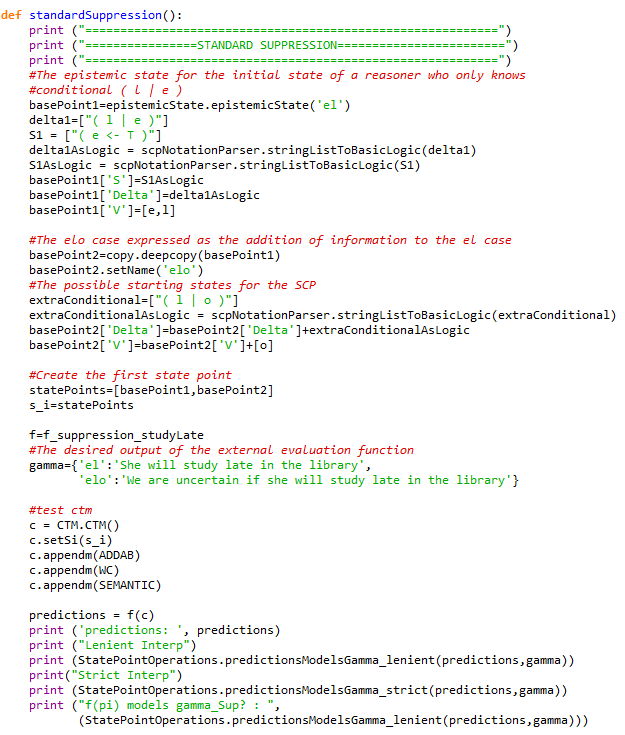
\includegraphics[width=1.3\linewidth]{suppression_python}
\caption{Code snippet showing how the Suppression Task is modelled in the SCP Framework.}
\label{fig:sup_snippet}
\end{figure}

\FloatBarrier

\section*{Additional Tables}
\begin{table}[!htbp]
\begin{center}
\begin{tabular}{c | c c c c c c }
 & & $s_\text{WST}$ & \texttt{addAB} & \texttt{AddExp} & \texttt{wc} & \texttt{semantic}\\
\hline
 & 0 & -1 & -2 & -3 & -4 & -5\\
$s_\text{WST}$ & -1 & 3 & 2 & 1 & 0 & -1\\
\texttt{th} & -6 & -2 & 0.0 & -1.0 & -2.0 & -3.0
\end{tabular}
\caption{Extended Needleman-Wunsch comparison of $\mu_{D,3}$ to $\mu'_{D,7}$.}
\label{tbl:extal1}
\end{center}
\end{table}








\begin{table}[h!]
\begin{center}
\begin{tabular}{c | c c c c c c }
 & & $s_\text{WST}$ & \texttt{addAB} & \texttt{AddExp} & \texttt{wc} & \texttt{semantic}\\
\hline
 & 0 & -1 & -2 & -3 & -4 & -5\\
$s_\text{WST}$ & -1 & 3 & 2 & 1 & 0 & -1\\
\texttt{addAB} & -2 & 2 & 4 & 3 & 2 & 1\\
\texttt{addExp} & -3 & 1 & 3 & 5 & 4 & 3\\
\texttt{wc} & -4 & 0 & 2 & 4 & 6 & 5\\
\texttt{semantic} & -5 & -1 & 1 & 3 & 5 & 7
\end{tabular}
\caption{Extended Needleman-Wunsch comparison of $\mu_{D,3}$ to $\mu_{D,7}$.}
\label{tbl:extal2}
\end{center}
\end{table}

\newpage






\subsection*{SCP Abduction Results}\label{ssec:scpabres}
Epistemic states demonstrating that \texttt{addExp} can be used to model the individual case of the Suppression Task where Suppression is prevented. Shown for SCP:
\[\mu=(\pi,f_\text{sup}())\]
\[\pi = (s_\text{dev} \longmapsto \texttt{addAB} \longmapsto \texttt{addExp} \longmapsto \texttt{wc} \longmapsto \texttt{semantic} )\]

\subsubsection*{SCP Abduction Results for the Suppression Task: Inital State Point}





\begin{table}[!htbp]
\begin{center}
\begin{tabular}{| c | c | }
\hline
name: &$\textbf{'el'}$ \\
$S$ : & $[(e \leftarrow  \top )]$\\
$Delta$ : & $[(l | e)]$\\
$V$ : & $[(e:u), (l:u)]$\\
$R[abducibles]$ : & ${'abducibles': [(o \leftarrow  \top ), (o \leftarrow  \bot )]}$\\
\hline
\end{tabular}
\end{center}
\end{table}
\begin{table}[!htbp]
\begin{center}
\begin{tabular}{| c | c | }
\hline
name: &$\textbf{'elo'}$ \\
$S$ : & $[(e \leftarrow  \top )]$\\
$Delta$ : & $[(l | e), (l | o)]$\\
$V$ : & $[(e:u), (l:u), (o:u)]$\\
$R[abducibles]$ : & ${'abducibles': [(o \leftarrow  \top ), (o \leftarrow  \bot )]}$\\
\hline
\end{tabular}
\end{center}
\end{table}

\subsubsection*{SCP Abduction Results for the Suppression Task: Final State Point}

\FloatBarrier
\begin{table}[!htbp]
\begin{center}
\begin{tabular}{| c | c | }
\hline
name: &$\textbf{'el'}$ \\
$S$ : & $[(e \leftrightarrow  \top ), (l \leftrightarrow  (e \land  (\lnot  ab_1))), (ab_1 \leftrightarrow  \bot )]$\\
$Delta$ : & $[]$\\
$V$ : & $[(e:\top), (l:\top), (ab_1:\bot)]$\\
$R[abducibles]$ : & $[(o \leftarrow  \top ), (o \leftarrow  \bot )]$\\
$R[explanation]$ : & $[]$\\

\hline
\end{tabular}
\end{center}
\end{table}
\begin{table}[!htbp]
\begin{center}
\begin{tabular}{| c | c | }
\hline
name: &$\textbf{'el'}$ \\
$S$ : & $[(e \leftrightarrow  \top ), (l \leftrightarrow  (e \land  (\lnot  ab_1))), (ab_1 \leftrightarrow  \bot ), (o \leftrightarrow  \top )]$\\
$Delta$ : & $[]$\\
$V$ : & $[(e:\top), (l:\top), (ab_1:\bot)]$\\
$R[abducibles]$ : & $[(o \leftarrow  \top ), (o \leftarrow  \bot )]$\\
$R[explanation]$ : & $[(o \leftarrow  \top )]$\\

\hline
\end{tabular}
\end{center}
\end{table}
\begin{table}[!htbp]
\begin{center}
\begin{tabular}{| c | c | }
\hline
name: &$\textbf{'el'}$ \\
$S$ : & $[(e \leftrightarrow  \top ), (l \leftrightarrow  (e \land  (\lnot  ab_1))), (ab_1 \leftrightarrow  \bot ), (o \leftrightarrow  \bot )]$\\
$Delta$ : & $[]$\\
$V$ : & $[(e:\top), (l:\top), (ab_1:\bot)]$\\
$R[abducibles]$ : & $[(o \leftarrow  \top ), (o \leftarrow  \bot )]$\\
$R[explanation]$ : & $[(o \leftarrow  \bot )]$\\

\hline
\end{tabular}
\end{center}
\end{table}
\begin{table}[!htbp]
\begin{center}
\begin{tabular}{| c | c | }
\hline
name: &$\textbf{'el'}$ \\
$S$ : & $[(e \leftrightarrow  \top ), (l \leftrightarrow  (e \land  (\lnot  ab_1))), (ab_1 \leftrightarrow  \bot ), (o \leftrightarrow  (\top  \lor  \bot ))]$\\
$Delta$ : & $[]$\\
$V$ : & $[(e:\top), (l:\top), (ab_1:\bot)]$\\
$R[abducibles]$ : & $[(o \leftarrow  \top ), (o \leftarrow  \bot )]$\\
$R[explanation]$ : & $[(o \leftarrow  \top ), (o \leftarrow  \bot )]$\\

\hline
\end{tabular}
\end{center}
\end{table}
\begin{table}[!htbp]
\begin{center}
\begin{tabular}{| c | c | }
\hline
name: &$\textbf{'elo'}$ \\
$S$ : & $[(e \leftrightarrow  \top ), (l \leftrightarrow  ((e \land  (\lnot  ab_1)) \lor  (o \land  (\lnot  ab_2)))),$\\
&$ (ab_1 \leftrightarrow  (\lnot  o)), (ab_2 \leftrightarrow  (\lnot  e))]$\\
$Delta$ : & $[]$\\
$V$ : & $[(e:\top), (l:u), (o:u), (ab_1:u), (ab_2:\bot)]$\\
$R[abducibles]$ : & $[(o \leftarrow  \top ), (o \leftarrow  \bot )]$\\
$R[explanation]$ : & $[]$\\

\hline
\end{tabular}
\end{center}
\end{table}
\begin{table}[!htbp]
\begin{center}
\begin{tabular}{| c | c | }
\hline
name: &$\textbf{'elo'}$ \\
$S$ : & $[(e \leftrightarrow  \top ), (l \leftrightarrow  ((e \land  (\lnot  ab_1)) \lor  (o \land  (\lnot  ab_2))))$\\
&$, (ab_1 \leftrightarrow  (\lnot  o)), (ab_2 \leftrightarrow  (\lnot  e)), (o \leftrightarrow  \top )]$\\
$Delta$ : & $[]$\\
$V$ : & $[(e:\top), (l:\top), (o:\top), (ab_1:\bot), (ab_2:\bot)]$\\
$R[abducibles]$ : & $[(o \leftarrow  \top ), (o \leftarrow  \bot )]$\\
$R[explanation]$ : & $[(o \leftarrow  \top )]$\\

\hline
\end{tabular}
\end{center}
\end{table}
\begin{table}[!htbp]
\begin{center}
\begin{tabular}{| c | c | }
\hline
name: &$\textbf{'elo'}$ \\
$S$ : & $[(e \leftrightarrow  \top ), (l \leftrightarrow  ((e \land  (\lnot  ab_1)) \lor  (o \land  (\lnot  ab_2)))),$\\
& $(ab_1 \leftrightarrow  (\lnot  o)), (ab_2 \leftrightarrow  (\lnot  e)), (o \leftrightarrow  \bot )]$\\
$Delta$ : & $[]$\\
$V$ : & $[(e:\top), (l:\bot), (o:\bot), (ab_1:\top), (ab_2:\bot)]$\\
$R[abducibles]$ : & $[(o \leftarrow  \top ), (o \leftarrow  \bot )]$\\
$R[explanation]$ : & $[(o \leftarrow  \bot )]$\\

\hline
\end{tabular}
\end{center}
\end{table}
\begin{table}[!htbp]
\begin{center}
\begin{tabular}{| c | c | }
\hline
name: &$\textbf{'elo'}$ \\
$S$ : & $[(e \leftrightarrow  \top ), (l \leftrightarrow  ((e \land  (\lnot  ab_1)) \lor  (o \land  (\lnot  ab_2)))),$\\
&$(ab_1 \leftrightarrow  (\lnot  o)), (ab_2 \leftrightarrow  (\lnot  e)), (o \leftrightarrow  (\top  \lor  \bot ))]$\\
$Delta$ : & $[]$\\
$V$ : & $[(e:\top), (l:\top), (o:\top), (ab_1:\bot), (ab_2:\bot)]$\\
$R[abducibles]$ : & $[(o \leftarrow  \top ), (o \leftarrow  \bot )]$\\
$R[explanation]$ : & $[(o \leftarrow  \top ), (o \leftarrow  \bot )]$\\

\hline
\end{tabular}
\end{center}
\end{table}







%\include{Appendices/AppendixB}
%\include{Appendices/AppendixC}



\end{document}  
